\documentclass[10pt]{beamer}
% \documentclass[aspectratio=169]{beamer}

%%%%%%%%%%%%%%%%%%%%%%%%%%%%%%%%%%%%%
%% Select input file encoding:
%%   utf8   - UTF-8, nowadays standard on most operating systems
%%   latin1 - ISO-8859-1
\usepackage[utf8]{inputenc}
\usefonttheme[onlymath]{serif}
\usepackage[normalem]{ulem}
% grey after pause if [<+>] appended to itemize:
\setbeamercovered{invisible}
\setbeamercovered{%
	again covered={\opaqueness<1->{15}}}
%%%%%%%%%%%%%%%%%%%%%%%%%%%%%%%%%%%%%
%% Select language
%%
% \usepackage[ngerman]{babel}        % Deutsch, neue Rechtschreibung
\usepackage[english]{babel}       % English

\usetheme{rwth}
\usepackage[T1]{fontenc}           % Font encoding (don't change!)
\usepackage{lmodern}               % Select Linux Modern Fonts (don't change)
% \usepackage{sansmathfonts}         % Sans fonts in math environments
\usepackage{textcomp}              % fix 'missing font symbols' warning
%\renewcommand{\rmdefault}{phv}     % Arial like (Helvetica)
%\renewcommand{\sfdefault}{phv}     % Arial like (Helvetica)
\usepackage[scaled=0.92]{helvet}
% \usepackage[default]{lato}

\usepackage[ddmmyyyy]{datetime}
\renewcommand{\dateseparator}{.}

%% graphics related packages
\usepackage{graphicx}              % needed to include graphics (don't change)
\usepackage{epstopdf}              % required to include eps files
%\usepackage{svg}                   % include svg files (requires Inkscape)
\usepackage[encoding,filenameencoding=utf8]{grffile} % allow utf8 file names in graphics

%%%%%%%%%%%%%%%%%%%%%%%%%%%%%%%%%%%%%
%% import packages for content
%%
%\usepackage{listings}                           % for lstlisting and \lstinline|..|
%\usepackage{minted}
%% TikZ can be used to /program/ graphics.
\usepackage{tikz}                                % comment-out, if you don't need this.
%% some TikZ-libraries and settings for the examples...
\usetikzlibrary{shadings}           % GW: color gradients
\usetikzlibrary{arrows,calc,positioning,fit,matrix,shadows,chains,arrows,shapes,spy,fadings}
\usepackage{pgfplots}
\usetikzlibrary{pgfplots.units,shapes.symbols,shapes.arrows}
%\usetikzlibrary{pgfplots.external}
%\tikzexternalize[prefix=tmp/]

%%%%%%%%%%%%%%%%%%%%%%%%%%%%%%%%%%%%%%%%%%%%%%%%%%%%%%%%%%%%%%%%%%%%%%%%%%%%%%%
%% Custom packages and definitions

% Mathematikumgebung
\usepackage{amsmath}
\usepackage{amssymb}
\usepackage{sansmath}

% tabularx -> bessere "tabular"-Umgebung
\usepackage{tabularx}

% zusätzliche Formatbezeichner für die tabularx-Umgebung
\newcolumntype{L}{>{\raggedright\let\newline\\\arraybackslash\hspace{0pt}}X}
\newcolumntype{R}{>{\raggedleft\let\newline\\\arraybackslash\hspace{0pt}}X}
\newcolumntype{C}{>{\centering\let\newline\\\arraybackslash\hspace{0pt}}X}

% center text vertically in tabularx(column)
%\renewcommand{\tabularxcolumn}[1]{>{\large}m{#1}}

% Bessere Tabellenlinien
\usepackage{booktabs}

% Tabellenzeilen für booktabs anpassen -> call on frame with table
\newcommand{\fixbooktabsrowhight}{%
  \setlength{\aboverulesep}{0pt}
  \setlength{\belowrulesep}{0pt}
  \setlength{\extrarowheight}{.5ex}
}

% Zellen über mehrere Zeilen
\usepackage{multirow}
\usepackage{hhline}

\DeclareMathOperator\LSTM{LSTM}
\DeclareMathOperator\LayerNorm{LayerNorm}
\DeclareMathOperator\SelfAttention{SelfAttention}
\DeclareMathOperator\Attention{Attention}
\DeclareMathOperator\FC{FC}
\DeclareMathOperator\Feedforward{Feedforward}
\DeclareMathOperator\Activation{Activation}
\DeclareMathOperator\ReLU{ReLU}
\DeclareMathOperator\softmax{softmax}
\DeclareMathOperator\RNN{RNN}
\DeclareMathOperator\RNNCell{RNNCell}
\DeclareMathOperator\Encoder{Encoder}
\DeclareMathOperator\Decoder{Decoder}
\DeclareMathOperator\argmax{argmax}
\DeclareMathOperator\simi{sim}
\DeclareMathOperator\Concat{Concat}


\DeclareMathOperator\E{E}
\DeclareMathOperator\Var{Var}
% Source, e.g. for images
\setbeamercolor{framesource}{fg=gray}
\setbeamerfont{framesource}{size=\tiny}

\usepackage[absolute,overlay]{textpos}
\newcommand{\source}[1]{\begin{textblock*}{\linewidth}(1ex,\paperheight-2.75em)
  \begin{beamercolorbox}[left]{framesource}
    \usebeamerfont{framesource}\usebeamercolor[fg]{framesource} Source: {#1}
  \end{beamercolorbox}
\end{textblock*}}

\usepackage{etoolbox}
%% short titles for toc \(sub)section[SHORTTITLE for toc]{LONGTITLE for slide}
\makeatletter
% Insert [short title] for \section in ToC
\patchcmd{\beamer@section}{{#2}{\the\c@page}}{{#1}{\the\c@page}}{}{}
% Insert [short title] for \section in Navigation
\patchcmd{\beamer@section}{{\the\c@section}{\secname}}{{\the\c@section}{#1}}{}{}

%%%%%%%%%%%%%%%%%%%%%%%%%%%%%%%%%%%%%%%%%%%%%%%%%%%%%%%%%%%%%%%%%%%%%%%%%
% For Python code block
%
% taken from: https://tex.stackexchange.com/questions/83882/how-to-highlight-python-syntax-in-latex-listings-lstinputlistings-command
%
%%%%%%%%%%%%%%%%%%%%%%%%%%%%%%%%%%%%%%%%%%%%%%%%%%%%%%%%%%%%%%%%%%%%%%%%%
\DeclareFixedFont{\ttb}{T1}{txtt}{bx}{n}{8} % for bold
\DeclareFixedFont{\ttm}{T1}{txtt}{m}{n}{8}  % for normal

% Custom colors
\usepackage{color, colortbl}
% \definecolor{deepblue}{rgb}{0,0,0.5}
\definecolor{deepblue}{RGB}{0, 0, 128}
\definecolor{deepred}{rgb}{0.6,0,0}
%\definecolor{deepgreen}{rgb}{0,0.5,0}
\definecolor{deepgreen}{RGB}{0,128,0}

\definecolor{maroon}{cmyk}{0, 0.87, 0.68, 0.32}
\definecolor{halfgray}{gray}{0.55}
\definecolor{ipython_frame}{RGB}{207, 207, 207}
\definecolor{ipython_bg}{RGB}{247, 247, 247}
\definecolor{ipython_red}{RGB}{186, 33, 33}
\definecolor{ipython_green}{RGB}{0, 128, 0}
\definecolor{ipython_cyan}{RGB}{64, 128, 128}
\definecolor{ipython_purple}{RGB}{170, 34, 255}
\definecolor{pycharm_self}{RGB}{148, 85, 141}
\definecolor{pycharm_init}{RGB}{178, 0, 178}
\definecolor{pycharm_deco}{RGB}{0, 0, 178}
\definecolor{pycharm_number}{RGB}{0, 0, 255}
\definecolor{pycharm_comment}{RGB}{128, 128, 128}
\definecolor{LightCyan}{rgb}{0.88,1,1}
\definecolor{applegreen}{rgb}{0.55, 0.71, 0.0}
\definecolor{cream}{rgb}{1.0, 0.99, 0.82}
\usepackage{listings}

% Python style for highlighting
\newcommand\pythonstyle{\lstset{
language=Python,
basicstyle=\footnotesize\ttm,
backgroundcolor=\color{mygray},
numbers=left,
%commentstyle=\color{ipython_cyan}\ttm,
commentstyle=\color{pycharm_comment}\ttm,
otherkeywords={None, False, True, with},
keywordstyle=\ttb\color{deepblue},
emph={__init__},
emphstyle=\color{pycharm_init},
emph={[2]self},
emphstyle=[2]\color{pycharm_self},
emph={[3]super},
emphstyle=[3]\color{pycharm_deco},
alsoletter={1234567890},
% emph={[4]1,2,3,4,5,6,7,8,9,0},
% emphstyle=[4]\color{pycharm_number},
% morekeywords=[3]{14, 1, 2, 3, 4, 5, 6, 7, 8, 9, 0},
% keywordstyle=[3]{\color{pycharm_number}},
stringstyle=\color{deepgreen},
%frame=tb,                         % Any extra options here
showstringspaces=false            % 
}}


% Python environment
\lstnewenvironment{python}[1][]
{
\pythonstyle
\lstset{#1}
}
{}

% Python for external files
\newcommand\pythonexternal[2][]{{
\pythonstyle
\lstinputlisting[#1]{#2}}}

% Python for inline
\newcommand\pythoninline[1]{{\pythonstyle\lstinline!#1!}}
%%%%%%%%%%%%%%%%%%%%%%%%%%%%%%%%%%%%%%%%%%%%%%%%%%%%%%%%%%%%%%%%%

% disable PDF navigation icons
\setbeamertemplate{navigation symbols}{}

%%%%%%%%%%%%%%%%%%%%%%%%%%%%%%%%%%%%%%%%%%%%%%%%%%%%%%%%%%%%%%%%%
% irie: Arial font as recommended by USI.
% but only work with xelatex!
% comment these two lines out, if needed...
%\usepackage{fontspec}
%\setmainfont{Arial}

% more shortcut
\newcommand{\code}[1]{\texttt{#1}}
\newcommand{\codeb}[1]{\colorbox{mygray}{\texttt{#1}}}
\newcommand{\link}[1]{{\footnotesize \url{#1}}}
\newcommand{\alertbf}[1]{\textbf{\alert{#1}}}
\newcommand{\emphbf}[1]{\textcolor{myblue}{\textbf{#1}}}
\newcommand{\citem}[1]{{\footnotesize \textcolor{myblue}{\cite{#1}}}}

\newcommand{\vsp}{\vspace{2mm}}
\newcommand{\TODO}{{\textcolor{red}{TODO }}}

%%%%%%%%%%%%%%%%%%%%%%%%%%%%%%%%%%%%%%%%%%%%%%%%%%%%%%%%%%%%%%%%%%%%%%%%%%%%%%%
%
%  For title page
%
%%%%%%%%%%%%%%%%%%%%%%%%%%%%%%%%%%%%%%%%%%%%%%%%%%%%%%%%%%%%%%%%%%%%%%%%%%%%%%%
\title[Deep Learning Lab 2022]{\LARGE Deep Learning Lab}
\subtitle{}
\author{Instructor: Kazuki Irie\\ TAs: R\'obert Csord\'as, Aditya Ramesh}
\email{\scriptsize{\texttt{kazuki.irie@usi.ch}, \texttt{robert.csordas@idsia.ch}, \texttt{aditya.ramesh@idsia.ch}}} % optionally
\institute{The Swiss AI Lab IDSIA, USI \& SUPSI}
\date{First version: 19.09.2022, \alert{Last modified: \today/\currenttime} \\ 
Fall 2022, USI.}
% Fall semester 2020-2021, Universit\`a della Svizzera italiana}

% Logos
\logo{\vskip-2mm
\includegraphics[width=20mm]{logos/usi-h-10mm}\hspace{-2mm}} % optionally
\instlogo{\hspace{-3mm}
\includegraphics[height=10mm]{logos/idsia-logo-with-text}}

%%%%%%%%%%%%%%%%%%%%%%%%%%%%%%%%%%%%%%%%%
% Define section start style
% `sectitle` for a page with just title.
% `fulltoc`
% `sectoc`
\secstart{sectoc}

\begin{document}
\tableofcontents[]  % shows the outline.

\section*{Introduction}
\begin{frame}{Deep Learning Lab: Welcome}
\textbf{Structure and objectives:}
  \begin{itemize}
\item Acquire hands-on experience - \textit{Lab}!
\item Focus on practical aspects of machine learning/deep learning\\
($\approx$ 50\% lectures, 50\% exercises)
\item (Originally designed to) Complement the lecture \textit{Machine Learning}
\item But self-contained.
% \item Otherwise designed for broad audience.
\end{itemize}

\vspace{5mm}
\textbf{Introduction to:}
\begin{itemize}
\item Framework, tools, implementation (PyTorch)
\item Basic \textbf{practicalities} of deep learning:
workflow, hyper-parameter tuning, practical tricks...
\item ...using various types of problems and model architectures
\item Learning to autonomously search for knowledge/solution to problems
\end{itemize}

%Share our knowledge based on experiences in coding, tuning, problem solving...\\
%Many of what we will tell are recommendations, suggestions.\\
%Practice has no absolutely right answers/approach.
%In the end of this lecture, we would like you to be able to...
\end{frame}

% Schedule 2019:
% Topic 1: 1 - 19. (20/09) + Act 1. # intro: applications, python, virtualenv, numpy, colab, TF.
% Topic 2: 20 - 30. (27/09) + Act 2.  # TF basics.
% Topic 3: 31 - 38. (04/10 and 11/10) + Act 3 # Start: fundamental models, linear regression. 
% Topic 4: 39 - 49. (18/10) + Act 4  # classification, FFNN, MNIST.
% Topic 5: 50 - 60. (25/10) + Act 5  # CNN, MNIST again.
% Topic 6: 61 - 74. (08/11) + Act 6  # RNN, n-back.
% Topic 7: 75 - 85. (15/11 and 22/11) + Act 7  # LSTM, n-back again.
% Topic 8: 86 - 98. (29/11, 06/12, 13/12, 20/12)  # selected models + RL?
% Act 8 distributed on 06/12.

% i.e. Act 3 and 7 takes the whole day. + Act 8 multiple days?

% Schedule 2020:
% Room A21.
% 14 days.
% Tentative plan: 7 1/2 days exercises + 6 1/2 days lectures?
% 01 - 13. (18/09): Intro + Act 1 (Python basics).
% (25/09): [Change order? introduce PyTorch basics first??] + Act 2 (PyTorch basics?)
% (02/10): workflow overview
% Topic 3:  (02/10 and 9/10)
% (9/10): 
% Topic 4:  (16/10)
% Topic 5:  (23/10)
% Topic 6:  (30/10)
% Topic 7:  (06/11 and 13/11)
% Topic 8:  (20/11, 27/11, 4/12, 11/12, 18/12)

% ===================
%  Lecture contents:
% ===================
% Intro (half) 1 - 13++
% Workflow (full day) 14 - 30
% PyTorch  basics (full) Tensor manipulation + Auto diff. 31 - 62
% Implementation of systems, whole pipeline, FF model, MNIST. 63 - 85 --> E4.
% Start: fundamental blocks: CNN. 86 - 100. --> E5/A2.

% RNN, residual connections. 101 - 109.
% Attention, self-attention, Transformers: 110 - 121.
% Start: Practical tricks.  122 - 135.
% Start: Building models. encoder-decoder 136 - 146
% enc-dec + attention: 147 - 154.
% Summary & final words: 155 - 165.

% ===================
%  Exercises:
% ===================
% E1: Intro to Python, Colab etc. (half?)
% E2: Intro to PyTorch?? Basic Tensor manipulation? (full?)
% E3/A1: First PyTorch applied exercise? regression? (full?)
% E4: MNIST FF model + extra (half? make it full?)
% E5/A2: CNN CIFAR (full?)
% E6: RNN basics (half?)
% E7/A3: Language modeling (RNN + Trafo?) (full)
% E8/A4: Final deepmind math. (full or more?)


% Put assignments one week before the dedicated session,
% leave them 2 weeks after the session to finish.
% (total 3 weeks.)

% Tentative plan:
% (18/09): Intro + E1 (Python basics).
% (25/09): Workflow (full day) 14 - 30, + PyTorch basics?
% (02/10): PyTorch  more example, regression + E2.
% (9/10): E3/A1.

% (16/10): Implementation of systems, whole pipeline, FF model, MNIST. 63 - 85 --> E4.
% (23/10): Start: fundamental blocks: CNN. 86 - 100. --> distribute E5/A2.
% (30/10): E5/A2.

% (06/11): RNN, residual connections. 101 - 109. + E6
% (13/11): Attention, self-attention, Transformers: 110 - 121. no exercise.
% (20/11): E7/A3.

% (27/11): Practical tricks.  122 - 135. no exercise?
% (4/12): Building models. encoder-decoder 136 - 146 + attn 147 - 154. --> distribute E8/A4.
% (11/12): E8/A4.

% (18/12): Summary & final words: 155 - 165.

\begin{frame}{Course Logistics}
%\vspace{-3mm}
\textbf{Time and location:}
\begin{itemize}
\item \textbf{Mondays from 10:30 to 12:00} (no break in principle)
\item Lecture room: \textbf{C1.03} Est Campus \link{https://www.desk.usi.ch/en/lugano-campus-map-access-facilities}
\end{itemize}
\pause
\vsp
\textbf{Format:}
  \begin{itemize}
\item 3 ETCS credits for Master (2 for PhD).
\item Lectures + guided exercises: 4 of these exercises are \alert{assignments}.
\item \textbf{Live streaming} on Microsoft Teams ``Deep Learning Lab 2022"\\
Use your USI account and access code: \textbf{ezdr8cr}\\
You can raise your hand for questions (but it may take some time for me to notice).
\item \textbf{All lectures/sessions will be recorded.}
\end{itemize}
\pause
\vsp
\textbf{Course materials:}
\begin{itemize}
\item All course materials (slides, exercise sheets) will be uploaded on \textbf{iCorsi3}. Slides will get gradually updated (pls. check the date/version).
\item Videos will be uploaded on \textbf{Panopto}.
\end{itemize}
\end{frame}

\begin{frame}{Course Logistics (cont'd)}
\vspace{-5mm}
\textbf{No more special disposition related to COVID at USI}
\begin{itemize}
\item It is your decision to opt for wearing a mask in the classroom (or not).
\end{itemize}
\vsp
See the official announcement: \link{https://www.usi.ch/en/feeds/13812}
% The official text at \link{https://www.desk.usi.ch/en/covid-19-protection-provisions?_ga=2.165121663.1388650446.1599575576-1918497133.1599474081}
\end{frame}


\begin{frame}{Grading and Rules}
\vspace{-2mm}
\textbf{Grades:}
\begin{itemize}
\item Entirely determined by your performance on the \alert{4 assignments}!
\item Difficulty/length of assignments gradually increases.
\item Final grade: weighted average (15\%, 20\%, 25\%, and 40\%)
\item All assignments must be solved using Python and PyTorch.\\
(Solution in other languages will not be accepted).
\item More generally: \textbf{please respect rules specified in the assignments!}
\end{itemize}
\vsp
\pause
\textbf{Deadlines:}
\begin{itemize}
\item Each assignment has its dedicated presentation session:
\begin{itemize}
\item I will shortly present the contents of the assignments.
\item TA(s) and I stay available for your questions in the remaining time.
\end{itemize}
\item The assignments must be submitted \alert{within 2 weeks} from the session: \textbf{Sunday evening at 10:00 PM} (except for the last assignment).
\item All assignment/exercise sheets will be available on iCorsi3 (soon!).
\end{itemize}
%\textbf{Late submission policy:}
%\begin{itemize}
%\item Within
%\item You must individually submit \textbf{your own solution}.
%\item In case of plagiarism: score of 0 for everyone involved.
%\end{itemize}
%\vsp
%\pause
%\textbf{Collaboration policy:}
%\begin{itemize}
%\item You may discuss with each other, \textbf{but}:
%\item You must individually submit \textbf{your own solution}.
%\item In case of plagiarism: score of 0 for everyone involved.
%\end{itemize}
%\vsp
%\pause
%\vsp
%\textbf{Attendance:}
%\begin{itemize}
%\item No attendance control. But: highly recommended to attend/watch all lectures!
%\end{itemize}
\end{frame}

\begin{frame}{Grading and Rules (cont'd)}
\textbf{Late submission policy:}
\begin{itemize}
\item Deadline Sunday 10:00 PM.
\item \textbf{10 min grace period}: no reduction if submitted between 10:00 - 10:10 PM.
\item \textbf{-30\% to your score} if submitted within 3 days after the deadline, i.e.\\
between Sunday 10:11 PM - Wednesday 10:00 PM.
\item 0 point if submitted later.
\end{itemize}
\vsp
\pause
\textbf{Collaboration policy:}
\begin{itemize}
\item You may discuss with each other, \textbf{but}:
\item You must individually submit \textbf{your own solution}.
\item In case of plagiarism: score of 0 for everyone involved (more on this later)
\end{itemize}
\pause
\vsp
\textbf{Course attendance:}
\begin{itemize}
\item Not mandatory.
\item But obviously: highly recommended to attend/watch all lectures!
\item Ask questions about the assignments in the dedicated Q/A sessions, not the day before the deadline!
\end{itemize}
\end{frame}

\begin{frame}{Plagiarism}
\begin{itemize}
\item Plagiarism can have very serious and unpleasant consequences.
\item[-] See USI's study regulation Art. 38. 1 and 2.\\ \link{ https://content.usi.ch/sites/default/files/storage/attachments/inf/inf-study-regulations-faculty-informatics-2013-2014-bachelor-master.pdf}
\vsp
\item Typical cases: lines of code or textual answers copied from the internet or from a colleague with minor modifications.
\item \alert{It is strictly forbidden to exchange your code with your colleagues in any form.}
\item[-] The whole point of this course is about learning to write your own code.
\item[-] You are allowed to use code presented in the lecture as your starting point. But nothing else should be copied.
\item[-] Unfortunately: last year 14 students out of 60 got 0 on Assignment 3 (especially unfortunate for good students who actually solved the problem but got 0 because they shared their code to others who plagiarized it).
\end{itemize}
\end{frame}

\begin{frame}{Grading and Rules (cont'd)}
\textbf{Reports:}
\begin{itemize}
\item For assignments, you will have to submit reports.
\item Please use \textbf{LaTeX} to write your report.
\item If you do not know \LaTeX\,\,yet, it's an opportunity to learn it!\\
\vsp
\textit{Learn LaTeX in 30 min}: \link{https://www.overleaf.com/learn/latex/Learn_LaTeX_in_30_minutes}
\item Should be useful for your future reports/articles/papers/theses\\ (not only for this course!)
\item Useful online tool, \textbf{Overleaf}: \link{https://www.overleaf.com/}
\end{itemize}
\vsp
\pause
\textbf{Contacting us:}
\begin{itemize}
\item Questions about assignments should be ideally asked during the dedicated sessions, but we also do answer questions by email (But you should not expect us to answer questions asked on the day of the deadline).
\item \alert{Important}: When you contact me, please ALWAYS put the two TAs in cc. (all email addresses are on page 1).
\end{itemize}
\end{frame}

%\begin{frame}{Plagiarism}
%\begin{itemize}
%\item Plagiarism can have very serious and unpleasant consequences. 
%\item See USI's study regulation Art. 38. 1 and 2.\\ \link{ https://content.usi.ch/sites/default/files/storage/attachments/inf/inf-study-regulations-faculty-informatics-2013-2014-bachelor-master.pdf}
%\vsp
%\item Typical cases: lines of code or textual answers copied from the internet or from a colleague with minor modifications.
%\item \textbf{You should never exchange your code with your colleagues.}
%\item The whole point of this course is about learning to write your own code.
%\item You are allowed to use code presented in the lecture as your starting point. But nothing else should be copied.
%\item Unfortunate statistics: last year 14 students out of 60 got 0 on Assignment 3 (especially unfortunate for good students who actually solved the problem but got 0 because they shared their code to others who plagiarized it).
%\end{itemize}
%\end{frame}

\begin{frame}{More on the rules}
\textbf{FAQ:}
\begin{itemize}
\item Q: \textit{Oh I've done my assignment in Keras, it's too late to change it to PyTorch. Can you still accept my solution, just for this time?}\\
\emphbf{A}: No, we only accept submission written in Python and PyTorch.
\pause
\item Q: \textit{I have too many assignments this week, can we postpone the deadline?}\\
\emphbf{A}: No. We publish the assignment (at least) two weeks in advance.
\pause
\item Q: \textit{Do you accept scan/picture of handwritten solution?}\\
\emphbf{A}: No, we only accept machine printed submissions. \\
\pause
\item Q: \textit{Can you give me 2 more hours? (``I'm copying the solution from a friend'')}\\
\emphbf{A}: No, we'll apply the late submission policy (Copying will result in 0 for both you and your friend). \\
\end{itemize}
\vsp
\pause
\textbf{Other remarks}:
\begin{itemize}
\item Please make use of our Q/A sessions to ask questions on assignments.
We will not help you in the last minutes.\\
Bad example: write to us a day before the deadline to complain about the assignment.
\end{itemize}
\end{frame}


\begin{frame}{2022 Provisional Planning}
\vspace{-5mm}
% this makes it hard to maintain the previous schedule with 4 assignments.
% --> reduce 1 assingments. multiple possibilities.
% - Possibility 1: make assignment 1 much shorter: solve it in class together.
% ask students to take a look at the exercise before attending the class
% A1 deadline Thrusday on the week  of 17. (or do we just skip this one from grading?)
% exercise 6 --> provide code for text generation, and let them play with it, a few thing to be completed.
% A3: use the provided code above, but replace the RNN cell, (maybe even AR transformer?).
\begin{table}[t]
\begin{center}
\hspace{-7mm}
\begin{tabular}{|c|c|c|c|}
\hline
\multicolumn{2}{|c|}{Dates} & 10:30 - 11:15 & $\approx$ 11:15 - 12:00  \\ \hline
September & 19  & Lecture (Intro) &  Exercise 1 \\ \cline{2-4}
        & 26  & \multicolumn{2}{c|}{Lecture (Sec.\,1 + begin Sec.\,2.1)} \\ \hline
October &  03  & Lecture (Sec.\,2.1) &  Exercise 2 \\ \cline{2-4}
% \hhline{*{4}{:=}:}
\hhline{|~|---|}
%      & 10  & \multicolumn{2}{c|}{ \cellcolor{cream} Exercise 3 / \textbf{Assignment 1}} \\  \cline{2-4}
      & 10  &  Lecture (Sec.\,2.2) &  \cellcolor{cream} Exercise 3 / \textbf{Assignment 1} \\ \cline{2-4}
      & 17  &  Lecture (Sec.\,3.1) & \textbf{Q/A Assign. 1} (\alert{cont'd}) \& Exercise 4  \\ \cline{2-4} \cline{2-4} \hhline{|~|---|}
%      & 23  &  \multicolumn{2}{c|}{Lecture (Sec.\,3.1)} \\ \cline{2-4}
% \hhline{|~|---|}
 & 24  &  \multicolumn{2}{c|}{\cellcolor{cream} Exercise 5 / \textbf{Assignment 2}} \\ \cline{2-4}
&  31  & Lecture (Sec.\,3.2) &  \textbf{Q/A Assign. 2} (\alert{cont'd}) \& Exercise 6 \\ \hline
% November &  7  & Lecture (Sec.\,3.2) &  Exercise 6 \\ \cline{2-4}
  November        &  7  & Lecture (Sec.\,3.3) & Exercise 6 (\alert{cont'd})\\ \cline{2-4}
\hhline{|~|---|}
         & 14  &  \multicolumn{2}{c|}{\cellcolor{cream} Exercise 7 / \textbf{Assignment 3}} \\ \cline{2-4}
& 21 &   Lecture (Sec. 4) & \textbf{Q/A Assign. 3} (\alert{cont'd}) \\  \cline{2-4} \hhline{|~|---|}
 & 28  &  \multicolumn{2}{c|}{\cellcolor{cream}}  \\  \cline{1-2}
% & 28  &  \multicolumn{2}{c|}{\cellcolor{cream} Exercise 8 / \textbf{Assignment 4} (maybe on Friday before, TBD) }  \\  \hline
% December & 10  &  \multicolumn{2}{c|}{\alert{No class}} \\ \cline{2-4}
December         &  05  &  \multicolumn{2}{c|}{\multirow{-2}{*}{\cellcolor{cream} \alert{No class}, Recorded Video: Exercise 8 / \textbf{Assignment 4}}} \\ \cline{2-4}
% December         &  05  &   \multicolumn{2}{c|}{\cellcolor{cream} \alert{No class}, Recorded Video: Exercise 8 / \textbf{Assignment 4}}  \\ \cline{2-4}
        & 12 & Lecture (Sec. 5 \& 6) & \textbf{Q/A Assign. 4}  \\ \cline{2-4}
& 19 &   \multicolumn{2}{c|}{\textbf{Q/A Assign. 4} (on request)} \\ \hline
% & 19 &  \multicolumn{2}{c|}{\alert{No class}} \\ \hline
\end{tabular}
\end{center}
\end{table}
% Tentative plan:
% (18/09): Intro + E1 (Python basics).
% (25/09): Workflow (full day) 14 - 30, no exercise. + PyTorch basics?
% (02/10): PyTorch  basics + E2.
% (9/10): E3/A1.

% (16/10): Implementation of systems, whole pipeline, FF model, MNIST. 63 - 85 --> E4.
% (23/10): Start: fundamental blocks: CNN. 86 - 100. --> distribute E5/A2.
% (30/10): E5/A2.

% (06/11): RNN, residual connections. 101 - 109. + E6
% (13/11): Attention, self-attention, Transformers: 110 - 121. no exercise.
% (20/11): E7/A3.

% (27/11): Practical tricks.  122 - 135. no exercise?
% (4/12): Building models. encoder-decoder 136 - 146 + attn 147 - 154. --> distribute E8/A4.
% (11/12): E8/A4.

% (18/12): Summary & final words: 155 - 165.
\end{frame}


\begin{frame}{2022 Provisional Planning (cont'd)}
\vspace{-5mm}
\begin{itemize}
\item The exact schedule from the end of November is still to be determined.
\item We will make a poll to find the dates later (toward the end of October once the class is settled after 6 weeks).
\item Anything after Nov. 28 in the previous slide is subject to change!
\end{itemize}
\end{frame}

%\begin{frame}{2022 Planning (provisional)}
%% \vspace{-9mm}
%\begin{table}[t]
%\begin{center}
%\begin{tabular}{|c|c|c|c|}
%\hline
%\multicolumn{2}{|c|}{Dates} & 10:30 - 11:15 & $\approx$ 11:15 - 12:15  \\ \hline
%September & 19  & Lecture (Intro) &  Exercise 1 \\ \cline{2-4}
%        & 26  & \multicolumn{2}{c|}{Lecture (Sec.\,1 + begin Sec.\,2.1)} \\ \hline
%October &  03  & Lecture (Sec.\,2.1) &  Exercise 2 \\ \cline{2-4}
%% \hhline{*{4}{:=}:}
%\hhline{|~|---|}
%      & 10  & \multicolumn{2}{c|}{ \cellcolor{cream} Exercise 3 / \textbf{Assignment 1}} \\  \cline{2-4}
%      & 17  &  Lecture (Sec.\,2.2) &  Exercise 4 \\ \cline{2-4}
%      & 24  &  Lecture (Sec.\,3.1) & Exercise 4 (\alert{cont'd}) \\ \cline{2-4} \cline{2-4}
%%      & 23  &  \multicolumn{2}{c|}{Lecture (Sec.\,3.1)} \\ \cline{2-4}
%% \hhline{|~|---|}
% & 31  &  \multicolumn{2}{c|}{\cellcolor{cream} Exercise 5 / \textbf{Assignment 2}} \\ \hline
%November &  7  & Lecture (Sec.\,3.2) &  Exercise 6 \\ \cline{2-4}
%         &  14  & Lecture (Sec.\,3.3) & Exercise 6 (\alert{cont'd})\\ \cline{2-4}
%\hhline{|~|---|}
%         & 21  &  \multicolumn{2}{c|}{\cellcolor{cream} Exercise 7 / \textbf{Assignment 3}} \\ \cline{2-4}
% & 28  &   \multicolumn{2}{c|}{\alert{No class}} \\  \hline
%         & 28  &   Lecture (Sec. 4) & Exercise 7 (\alert{cont'd}) \\  \hline \hhline{|~|---|}
%% December & 10  &  \multicolumn{2}{c|}{\alert{No class}} \\ \cline{2-4}
%December         &  05  & \alert{No class (one of the slots)} & \multicolumn{1}{c|}{\cellcolor{cream} Exercise 8 / \textbf{Assignment 4}} \\ \cline{2-4}
%        & 12  & \multicolumn{2}{c|}{\alert{No class?}}  \\ \cline{2-4}
%& 19 &   Lecture (Sec. 5 \& 6)& Exercise 8 (\alert{cont'd})  \\ \hline
%% & 19 &  \multicolumn{2}{c|}{\alert{No class}} \\ \hline
%\end{tabular}
%\end{center}
%\end{table}
%% Tentative plan:
%% (18/09): Intro + E1 (Python basics).
%% (25/09): Workflow (full day) 14 - 30, no exercise. + PyTorch basics?
%% (02/10): PyTorch  basics + E2.
%% (9/10): E3/A1.
%
%% (16/10): Implementation of systems, whole pipeline, FF model, MNIST. 63 - 85 --> E4.
%% (23/10): Start: fundamental blocks: CNN. 86 - 100. --> distribute E5/A2.
%% (30/10): E5/A2.
%
%% (06/11): RNN, residual connections. 101 - 109. + E6
%% (13/11): Attention, self-attention, Transformers: 110 - 121. no exercise.
%% (20/11): E7/A3.
%
%% (27/11): Practical tricks.  122 - 135. no exercise?
%% (4/12): Building models. encoder-decoder 136 - 146 + attn 147 - 154. --> distribute E8/A4.
%% (11/12): E8/A4.
%
%% (18/12): Summary & final words: 155 - 165.
%\end{frame}
%
%\begin{frame}{2020 Planning (tentative)}
%% \vspace{-9mm}
%\begin{table}[t]
%\begin{center}
%\begin{tabular}{|c|c|c|c|}
%\hline
%\multicolumn{2}{|c|}{Dates} & 16:30 - 17:15 & $\approx$ 17:15 - 18:00  \\ \hline
%September & 18  & Lecture (Intro) &  Exercise 1 \\ \cline{2-4}
%      & 25  & \multicolumn{2}{c|}{Lecture (Sec.\,1 + begin Sec.\,2.1)} \\ \hline
%October &  02  & Lecture (Sec.\,2.1) &  Exercise 2 \\ \cline{2-4}
%% \hhline{*{4}{:=}:}
%\hhline{|~|---|}
%      & 09  & \multicolumn{2}{c|}{ \cellcolor{cream} Exercise 3 / \textbf{Assignment 1}} \\  \cline{2-4}
%      & 16  &  Lecture (Sec.\,2.2) &  Exercise 4 \\ \cline{2-4}
%      & 23  &  Lecture (Sec.\,3.1) & Exercise 4 (\alert{cont'd}) \\ \cline{2-4}
%%      & 23  &  \multicolumn{2}{c|}{Lecture (Sec.\,3.1)} \\ \cline{2-4}
%\hhline{|~|---|}
%      & 30  &  \multicolumn{2}{c|}{\cellcolor{cream} Exercise 5 / \textbf{Assignment 2}} \\ \hline
%November &  06  & Lecture (Sec.\,3.2) &  Exercise 6 \\ \cline{2-4}
%         &  13  & Lecture (Sec.\,3.3) & Exercise 6 (\alert{cont'd})\\ \cline{2-4}
%\hhline{|~|---|}
%         & 20  &  \multicolumn{2}{c|}{\cellcolor{cream} Exercise 7 / \textbf{Assignment 3}} \\ \cline{2-4}
%         & 27  &   Lecture (Sec. 4) & Exercise 7 (\alert{cont'd}) \\ \hline
%December &  04  & \multicolumn{2}{c|}{\cellcolor{cream} Exercise 8 / \textbf{Assignment 4}} \\ \cline{2-4}
%\hhline{|~|---|}
%         & 11  &  \multicolumn{2}{c|}{\alert{No class}} \\ \cline{2-4}
%         & 18  &  Lecture (Sec. 5 \& 6)& Exercise 8 (\alert{cont'd}) \\ \hline
%\end{tabular}
%\end{center}
%\end{table}
%% Tentative plan:
%% (18/09): Intro + E1 (Python basics).
%% (25/09): Workflow (full day) 14 - 30, no exercise. + PyTorch basics?
%% (02/10): PyTorch  basics + E2.
%% (9/10): E3/A1.
%
%% (16/10): Implementation of systems, whole pipeline, FF model, MNIST. 63 - 85 --> E4.
%% (23/10): Start: fundamental blocks: CNN. 86 - 100. --> distribute E5/A2.
%% (30/10): E5/A2.
%
%% (06/11): RNN, residual connections. 101 - 109. + E6
%% (13/11): Attention, self-attention, Transformers: 110 - 121. no exercise.
%% (20/11): E7/A3.
%
%% (27/11): Practical tricks.  122 - 135. no exercise?
%% (4/12): Building models. encoder-decoder 136 - 146 + attn 147 - 154. --> distribute E8/A4.
%% (11/12): E8/A4.
%
%% (18/12): Summary & final words: 155 - 165.
%\end{frame}

\begin{frame}{Textbooks/ References/ Links}
\vspace{-3mm}
Many good materials are available \emphbf{free online}.\\
\vsp
For example:
\vsp
\begin{itemize}
\item Textbooks on \textbf{machine learning} in general.
\vsp
\begin{itemize}
\item Bishop (2006). Pattern Recognition and Machine Learning. {\small \url{https://www.microsoft.com/en-us/research/people/cmbishop/prml-book/}}
\vspace{-2mm}
\item Goodfellow et al. (2015) Deep Learning. ~{\small \url{https://www.deeplearningbook.org/}}
\vsp
\item Zhang et al. (2019). Dive into Deep Learning.
\\{\small \url{https://d2l.ai}}
\vsp
\item Graves (2012).\\ Supervised Sequence Labelling with Recurrent Neural Networks. {\small \url{https://www.cs.toronto.edu/~graves/preprint.pdf}}
\end{itemize}
\end{itemize}
%More specific references will be given later where it's relevant.\\
%This lecture also covers practical aspects which are not necessary in textbooks.
\end{frame}

\begin{frame}{Textbooks/ References/ Links (cont'd)}
	\vspace{-4mm}
\begin{itemize}
\item \textbf{Python}
\begin{itemize}
\item \link{https://docs.python.org/3/tutorial/}\\ \alert{Highly recommended to check ASAP if not already familiar with Python!} 
\item Downey (2015). Think Python. 2nd Edition. \\ \link{https://greenteapress.com/wp/think-python-2e/}
\item Official quick intro to \textbf{NumPy}. \alert{Same!}\\
\link{https://numpy.org/devdocs/user/quickstart.html}
% \item Justin Johnson's tutorial (Stanford) \link{https://cs231n.github.io/python-numpy-tutorial/}
\end{itemize}
\vsp
\item \textbf{PyTorch}
\begin{itemize}
\item Official tutorial: \link{https://pytorch.org/tutorials/}
\item Deep Learning with PyTorch: A 60 minute blitz\\
\link{https://pytorch.org/tutorials/beginner/deep_learning_60min_blitz.html}
%\item Andrew Ng's lecture (Stanford): {\small \url{https://cs230.stanford.edu/blog/pytorch/}}
\end{itemize}
\end{itemize}
\vspace{2mm}
\textbf{Exercises 1 and 2 will cover basics of Python/NumPy and PyTorch respectively.}
% \vspace{2mm}
% More specific references are also given later.\\
%\vspace{2mm}
%Again: this lectures' focus is practical aspects which you might not be able to learn only by reading textbooks.
\end{frame}

\begin{frame}{Computational Resources}
\vspace{-5mm}
Your laptop is not a good option to run experiments. There are exercises you can not solve on your laptop.
\vsp
\pause
\begin{itemize}
\item \textbf{Google Colab} \link{https://colab.research.google.com/notebooks/intro.ipynb}
\begin{itemize}
\item The default choice. Need to create a google account.
\item Good tool for interactive programming (similar to Jupyter notebook).\\
\item \emphbf{Free GPUs} available (\textit{Edit} $\rightarrow$ \textit{Notebook Settings}, and choose GPU).\\
\item In principle, all assignments are solvable using this resource. Warning: we only accept plain Python script. Please do not submit notebook file.
\end{itemize}
\vsp
\pause
\item \textbf{Kaggle} \link{https://www.kaggle.com/code}
\begin{itemize}
\item Backup option if you hit ``some'' utilization limit on Colab.
\item Need to confirm a phone number to access free GPUs.
\item \textit{Settings} on the right panel $\rightarrow$ \textit{Accelerator}, and choose GPU.\\
\end{itemize}
\vsp
\pause
\item \textbf{USI, ICS cluster} \link{https://intranet.ics.usi.ch/HPC}
\begin{itemize}
\item Good option if you do not like writing code on a notebook. 
\item Learning how to organize your experiments on a cluster is good.
\item You need to use/learn \textit{Slurm}. Also risk: the cluster can be down!
\end{itemize}
\end{itemize}
\vsp
\textbf{Please make sure that you can access Colab or Kaggle today.}
\end{frame}

%\begin{frame}{Computational Resources}
%\vspace{-5mm}
%\begin{itemize}
%\item \textbf{USI, ICS cluster}\\ \link{https://intranet.ics.usi.ch/HPC} \\
%\begin{itemize}
%\item Good option, especially you are interested in High Performance Computing.\\
%%See: \url{https://intranet.ics.usi.ch/HPC}\\
%\item Learning to organize your experiments using a HPC cluster\\ is a good practice to learn.
%\item You need to use/learn \textit{Slurm}.
%\end{itemize}
%\vsp
%\pause
%\item \textbf{Google Colab}
%{\small \url{https://colab.research.google.com/notebooks/intro.ipynb}}
%\begin{itemize}
%\item Also highly recommended.
%\item Need to create a google account.
%\item Good tool for interactive programming (similar to Jupyter notebook).\\
%\item \emphbf{Free GPUs} available (\textit{Edit} $\rightarrow$ \textit{Notebook Settings}, and choose GPU).\\
%\item In principle, all assignments are solvable using this resource. Warning: we only accept plain Python script. Please do not submit notebook file.
%\end{itemize}
%\vsp
%\pause
%\item \textbf{Your laptop}... 
%\begin{itemize}
%\item Not a good option to run experiments.
%\item There are exercises you can not solve on your laptop.
%\end{itemize}
%\end{itemize}
%\vsp
%\textbf{We will get an introduction to these options in the} \emphbf{exercise session today.}
%\end{frame}

\begin{frame}[fragile]{USI ICS Cluster}
\vspace{-5mm}
\begin{itemize}
\item General instructions: \link{https://intranet.ics.usi.ch/HPC}
\item You will get credentials to access the cluster today (\codeb{username} and password) .
\item Connect to a front node \texttt{hpc.ics.usi.ch} (or 195.176.181.122) using SSH, i.e., execute on a terminal: \codeb{ssh username@hpc.usi.ch}\\
(be careful with 0 vs. o vs. O when typing the password).
%\item When loging in for the first time, run:
%\texttt{/apps/python/intelpython3/bin/conda init}
%\item then log out once.
\item Job manager used at ICS is \textit{Slurm}
\end{itemize}
\end{frame}

\begin{frame}[fragile]{USI ICS Cluster, Slurm}
\vspace{-5mm}
\begin{itemize}
\item You have to learn basic commands of \textit{Slurm}, essentially:
\item[-] \codeb{squeue} to view jobs in the queue.
\item[-] \codeb{sbatch your\_script\_file.sh} to submit your job.
\item[-] \codeb{scancel \$JOB\_ID} to kill your job.
\item Correctly prepare \codeb{your\_script\_file.sh}. Example: 
\end{itemize}
\begin{python}
#!/bin/bash

#SBATCH --job-name="abc"
#SBATCH --output=abc.%j.out
#SBATCH --error=abc.%j.err
#SBATCH --partition=gpu
#SBATCH --time=00:15:00
#SBATCH --mem=4000
#SBATCH --exclusive

srun python my_code.py
\end{python}
where \codeb{my\_code.py} is your main Python code file.
\begin{itemize}
\item Check the \textit{partitions} on \link{https://intranet.ics.usi.ch/HPC}
\end{itemize}
% /apps/python/intelpython3/bin/conda activate DL-lab
\end{frame}

\begin{frame}{Who are we?}
We work in \textbf{Prof.~J\"urgen Schmidhuber's team} at\\
\vsp
\textbf{IDSIA - Dalle Molle Institute for Artificial Intelligence}
\begin{center}
    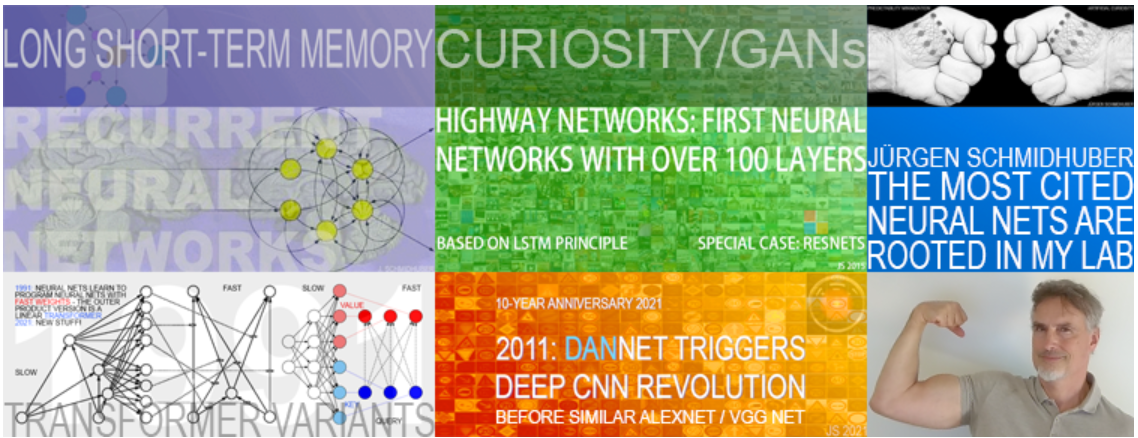
\includegraphics[height=0.5\textheight]{figures/idsia_lab.png}
\end{center}
\begin{itemize}
\item Lab with many historical contributions to deep learning and artificial intelligence\\
\link{https://people.idsia.ch/~juergen/most-cited-neural-nets.html}.
\item Affiliated with both USI and SUPSI.
\end{itemize}
\end{frame}

\begin{frame}{Your background?}
  \begin{itemize}
\item Undergraduate major?
\item Programming experience?
\item Python? C++?
\item Machine Learning? Neural networks?
\item Interest/application domain?
\end{itemize}
\vspace{2mm}
\pause
This is a course for a broad audience.\\
\vspace{2mm}
% We are also learning, and want to improve our lectures: feedback to...
But hopefully, you:
\begin{itemize}
% \item[-] be attending/have attended the lecture \textit{Machine Learning}.\\
\item[-] have interests! e.g., some vision of applications you are interested in.
\item[-] are ready to spend time for hands-on learning, e.g., debugging your code.
\end{itemize}
\end{frame}

\begin{frame}{Deep learning: impact on \\a wide range of applications}
\begin{minipage}{0.45\textwidth}
\emphbf{Image}
\begin{itemize}
\item Image classification
\item Object detection/segmentation
\item Image generation
% \item Image captioning
\item Image to image translation...
\end{itemize}
\begin{center}
    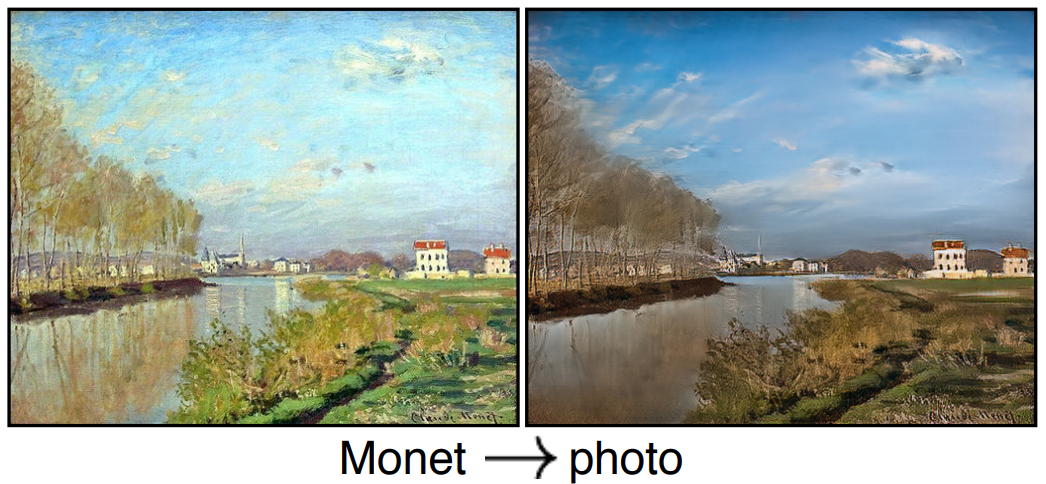
\includegraphics[height=0.3\textheight]{figures/applications/image_trans.png}
\end{center}
\vspace{-2mm}
\scriptsize{Input: Image/Paiting}\\
\scriptsize{Output: Image/Photo-realistic picture}
\end{minipage}
\begin{minipage}{0.45\textwidth}
\vspace{5mm}
\begin{center}
    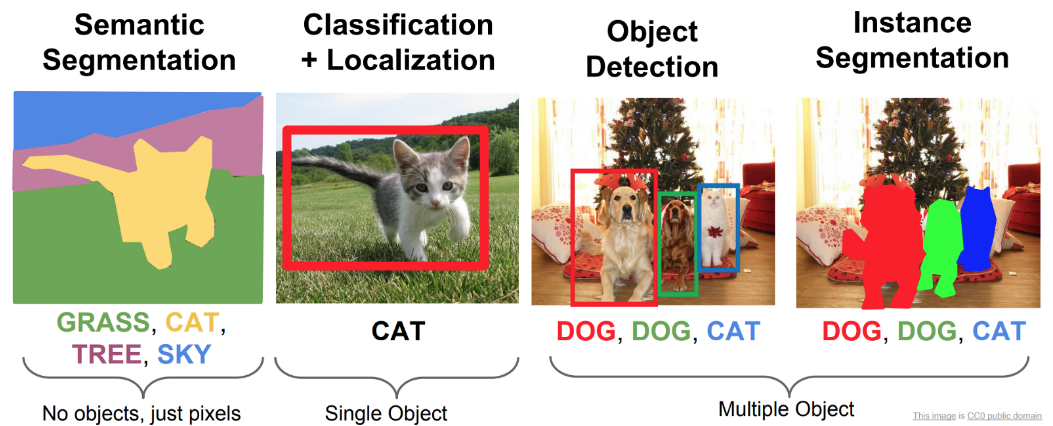
\includegraphics[height=0.35\textheight]{figures/applications/image_tasks.png}
\end{center}
% \vsp
\vspace{-2mm}
\begin{itemize}
\item Image captioning
\end{itemize}
\vspace{-5mm}
\begin{center}
    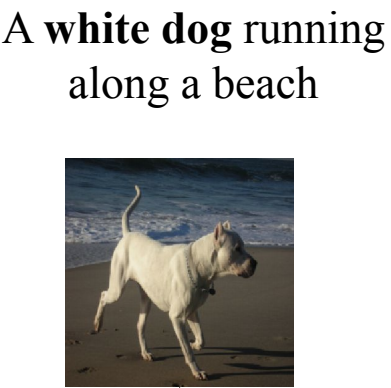
\includegraphics[height=0.3\textheight]{figures/applications/image_cap.png}
\end{center}
\vspace{-2mm}
\scriptsize{Input: Image} \\
\scriptsize{Output: Text describing the image}
 \vspace{3mm}
\end{minipage}
\hspace{5mm}
 {\footnotesize Images taken from \citem{nikolaus-etal-2019-compositional, ZhuPIE17, stanford2017}.}

%\begin{figure}
%  \begin{center}
%    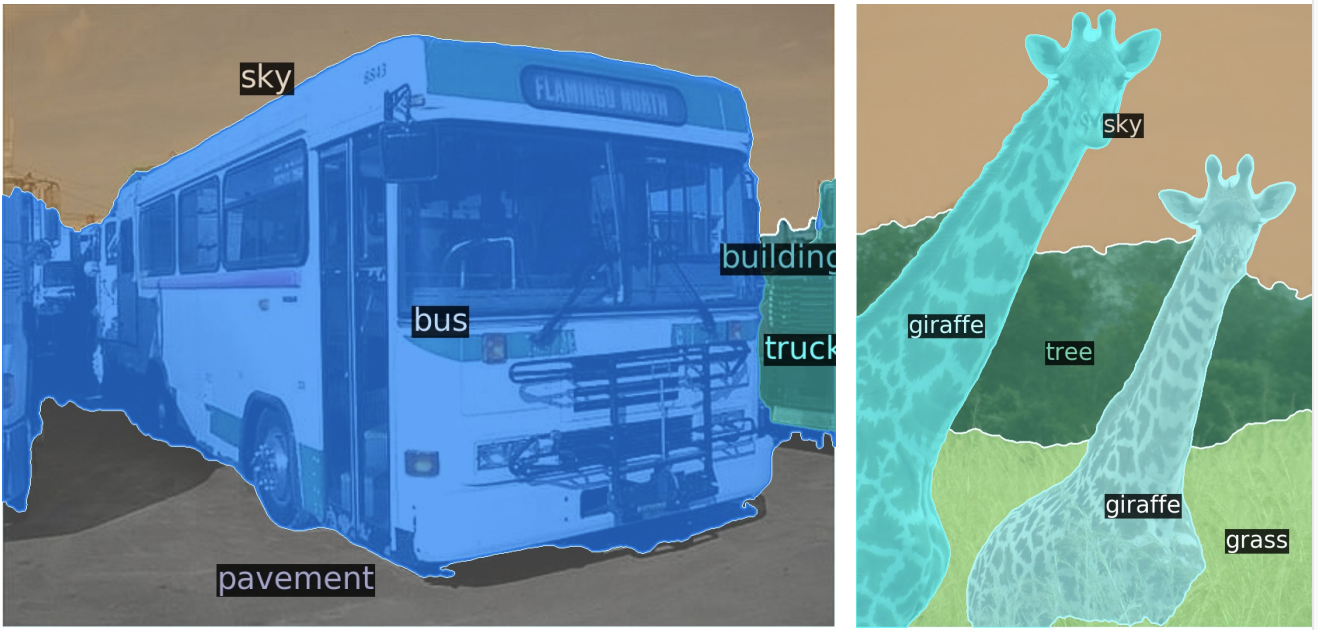
\includegraphics[height=0.5\textheight]{figures/applications/detr.png}
%  \end{center}
%\vspace{-2mm}
%\end{figure}
%    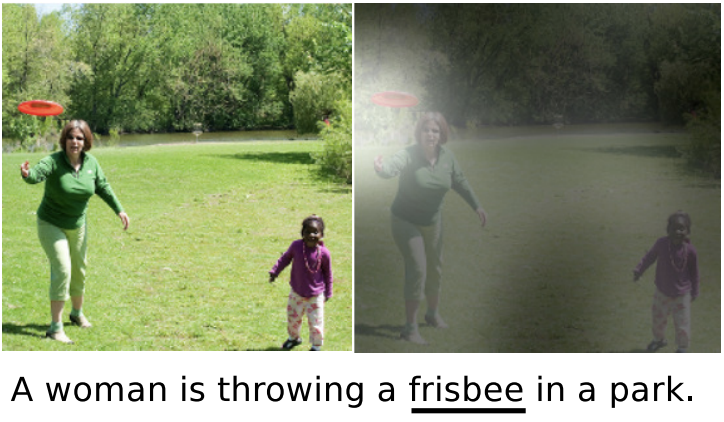
\includegraphics[height=0.3\textheight]{figures/applications/image-cap.png}
% \vspace{-2mm}
% {\small Images taken from \citem{carion2020end}.}
\end{frame}


\begin{frame}{Text to image (trending in 2022)}
%\begin{minipage}{0.45\textwidth}
\vspace{-5mm}
Imagen (Google, 2022) \link{https://imagen.research.google/}
\begin{center}
    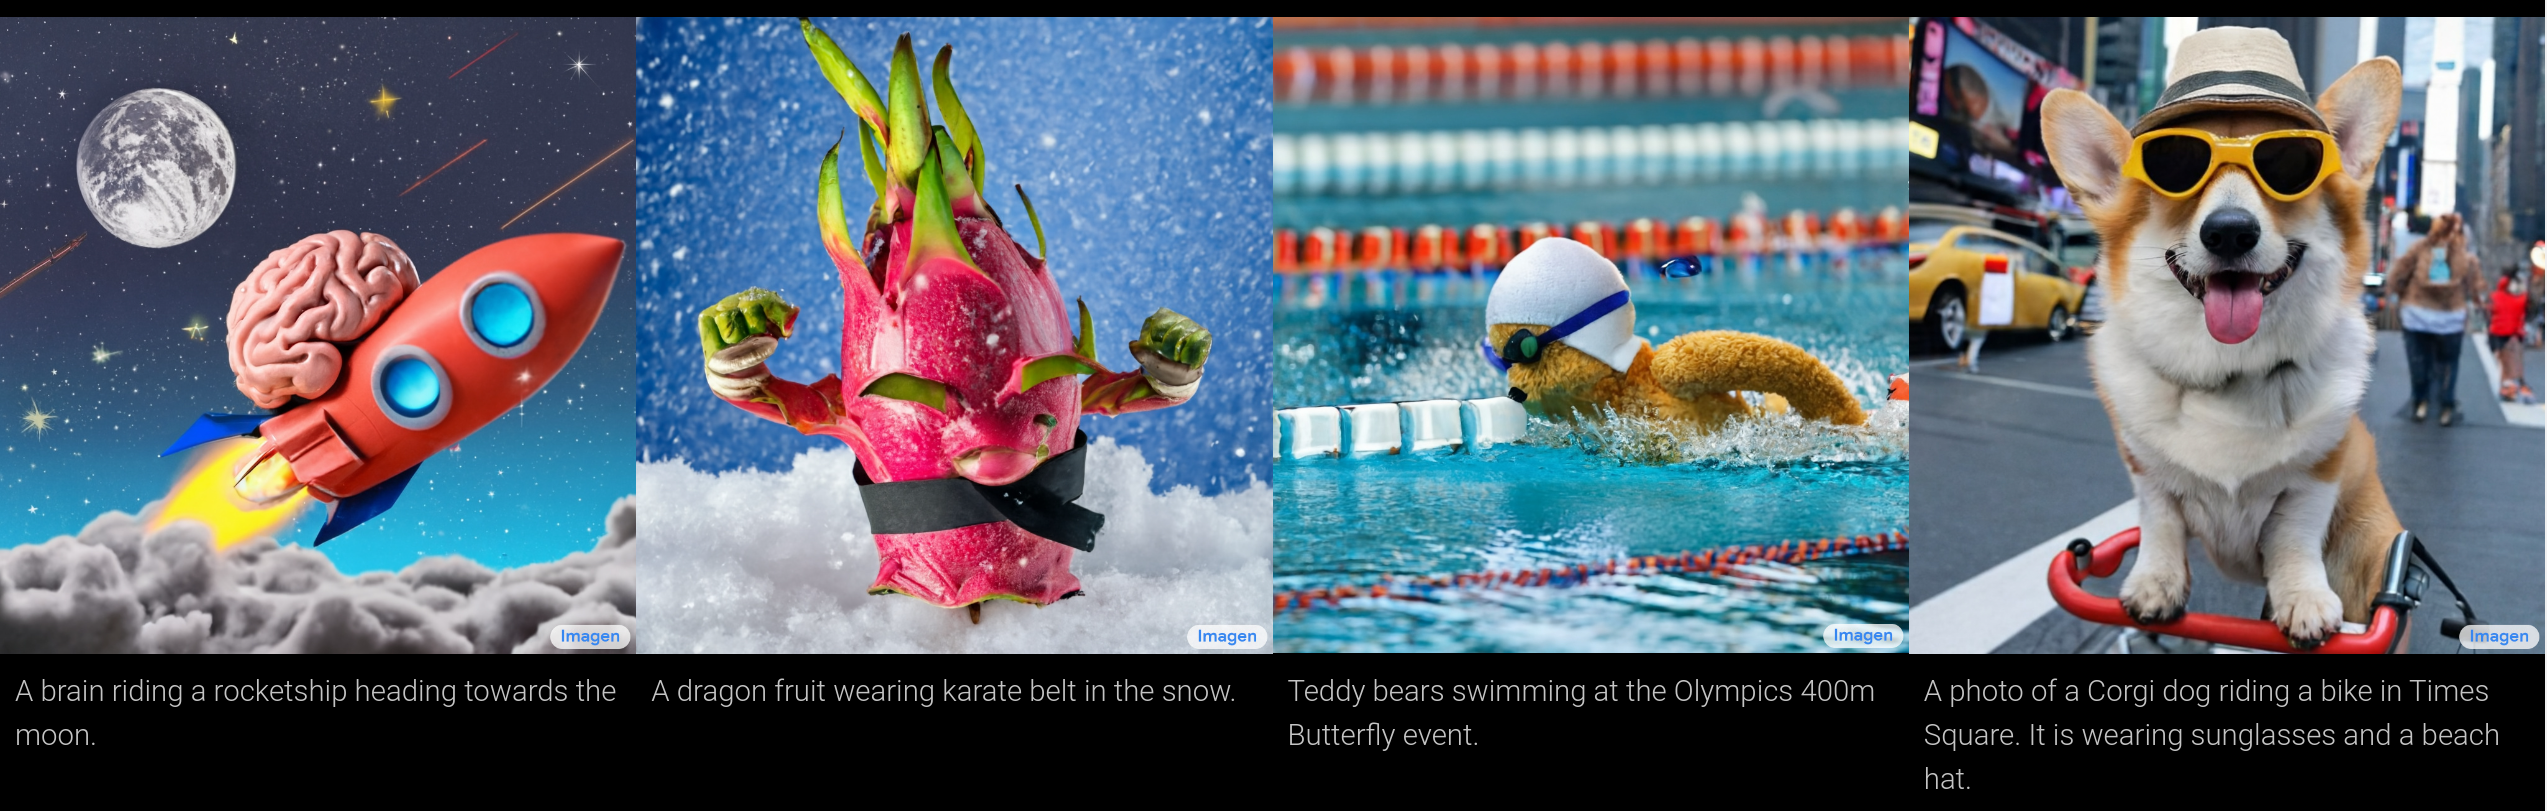
\includegraphics[height=0.5\textheight]{figures/applications/imagen_google.png}
%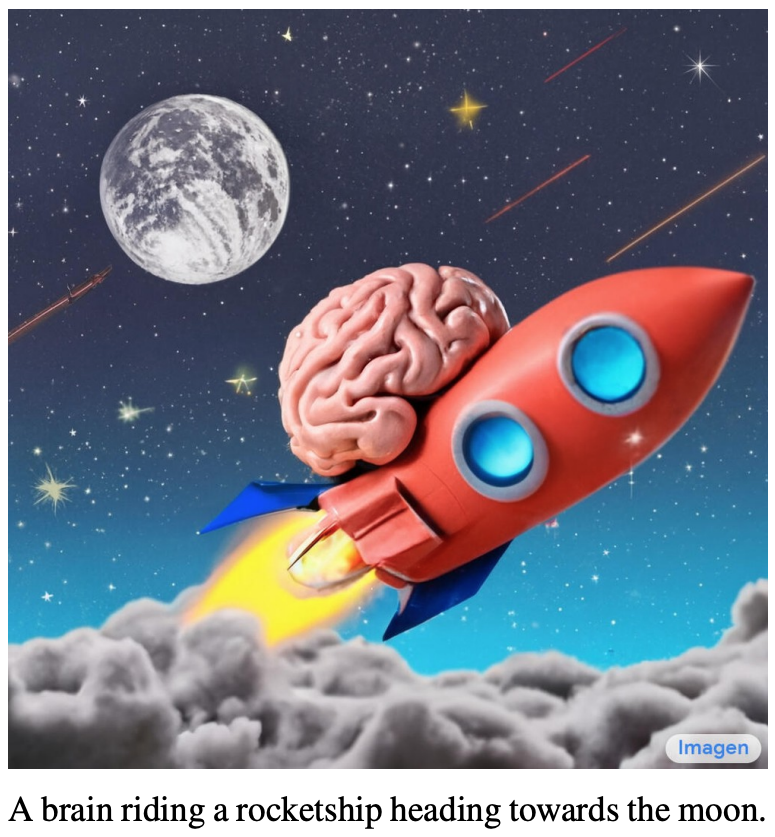
\includegraphics[height=0.5\textheight]{figures/applications/imagen_2.png}
%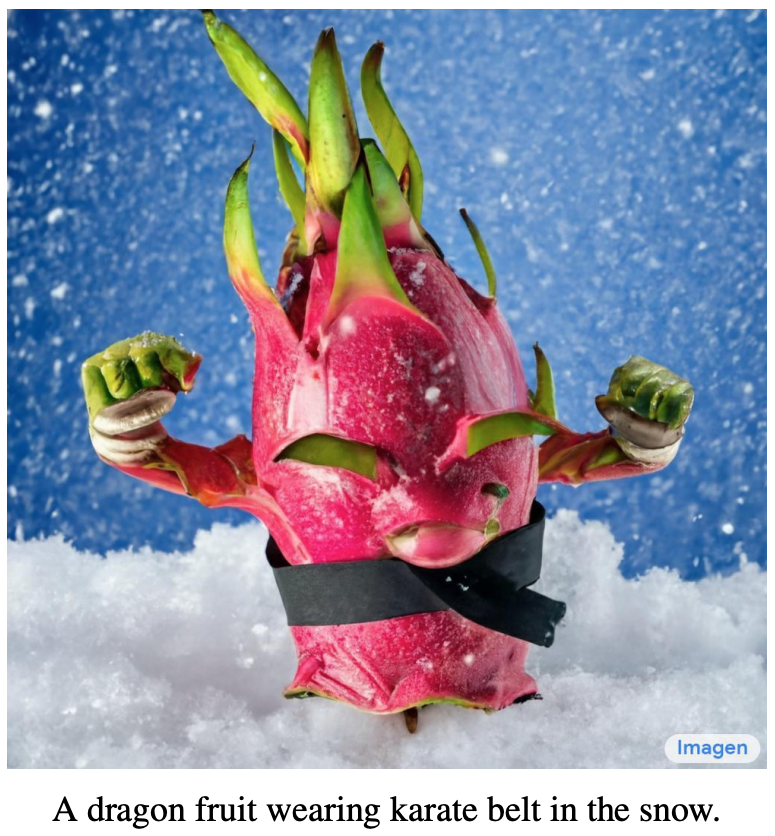
\includegraphics[height=0.5\textheight]{figures/applications/imagen_3.png}
\end{center}
%\begin{center}
%    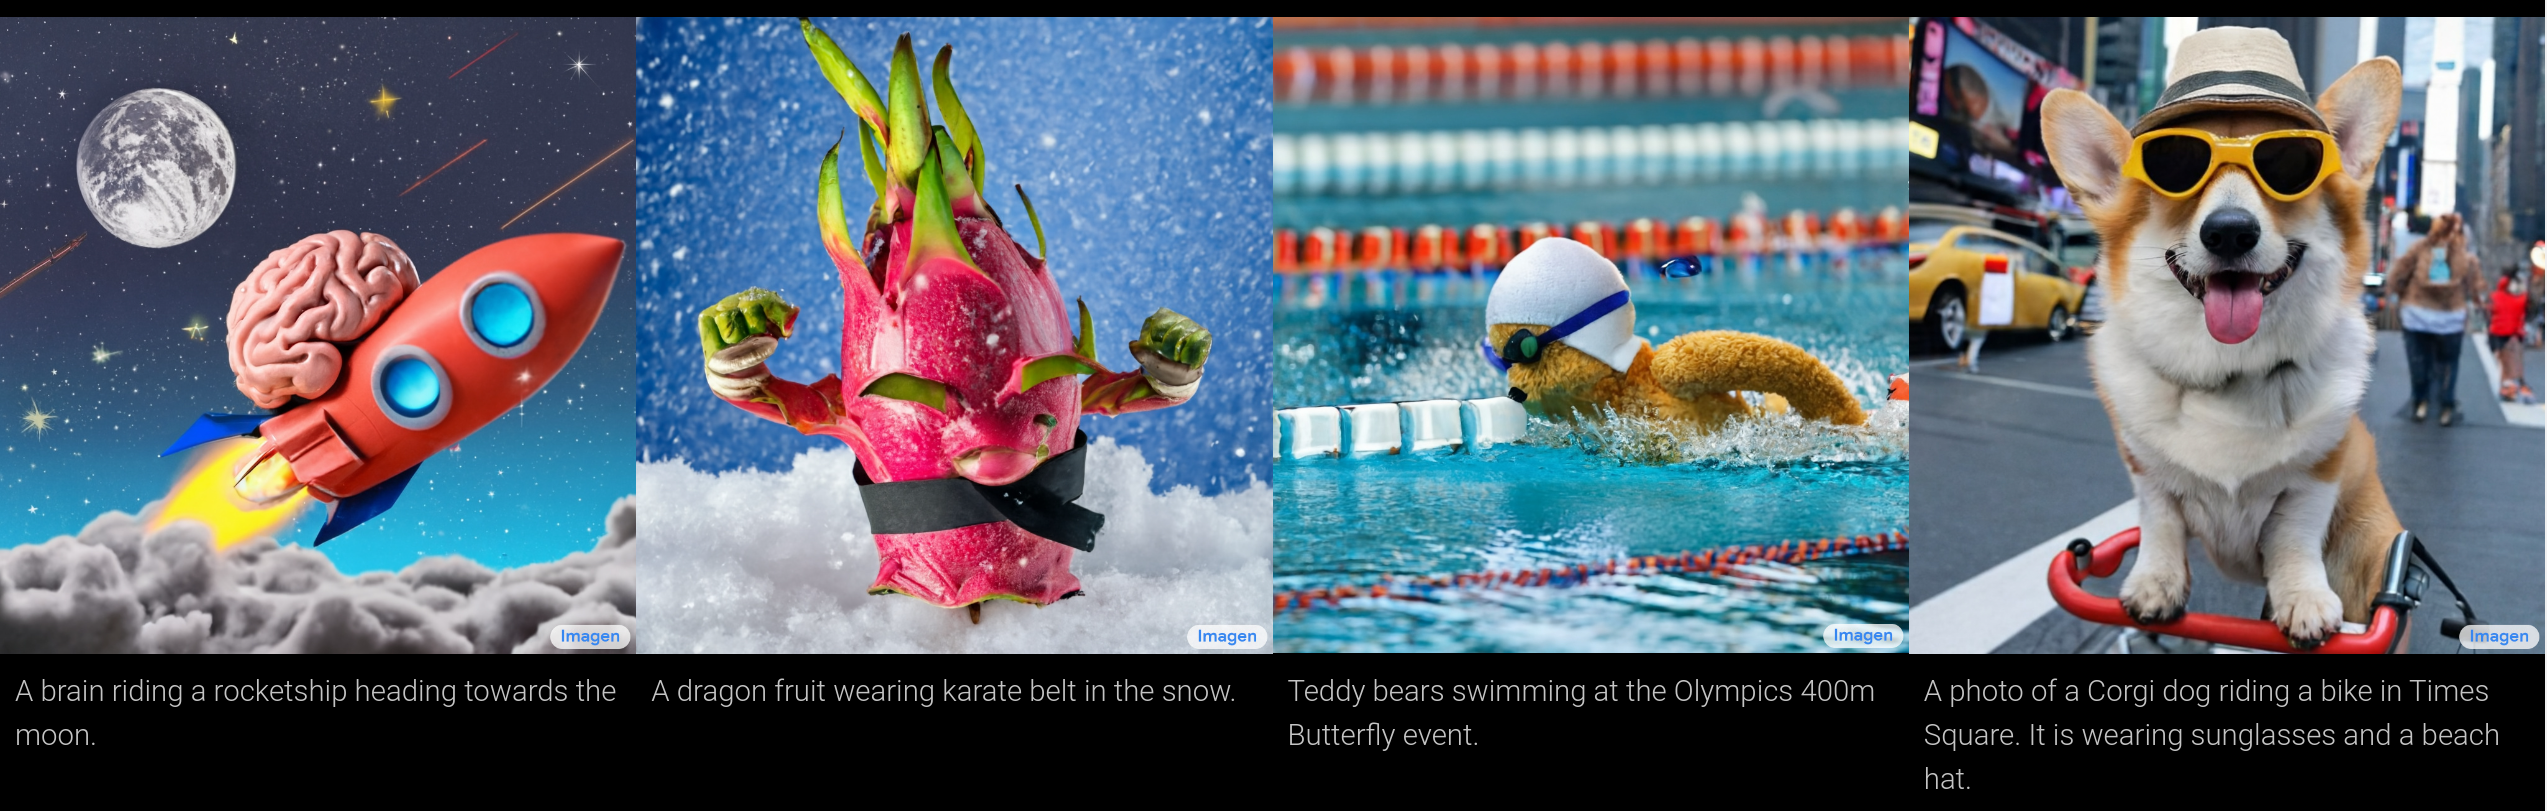
\includegraphics[height=0.5\textheight]{figures/applications/imagen_google.png}
%\end{center}
DALL-E 2 (OpenAI, 2022) \link{https://openai.com/dall-e-2/}
\begin{center}
\hspace{-20mm}
    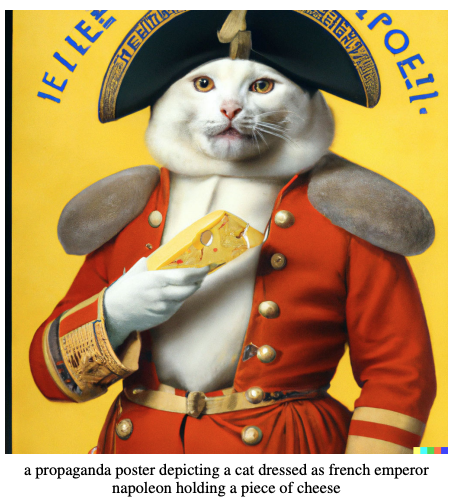
\includegraphics[height=0.4\textheight]{figures/applications/dalle2_1.png}
\hspace{10mm}
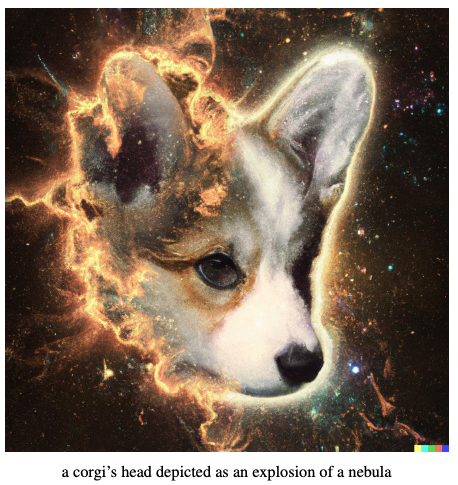
\includegraphics[height=0.4\textheight]{figures/applications/dalle2_3.png}
\hspace{10mm}
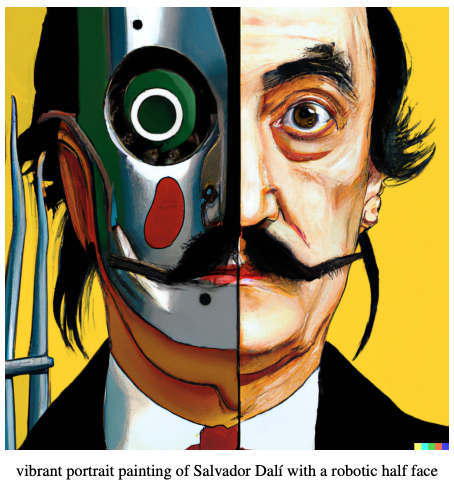
\includegraphics[height=0.4\textheight]{figures/applications/dalle2_2.png}
\end{center}
%\end{minipage}
%\begin{minipage}{0.45\textwidth}
%\vspace{5mm}
%\begin{center}
%    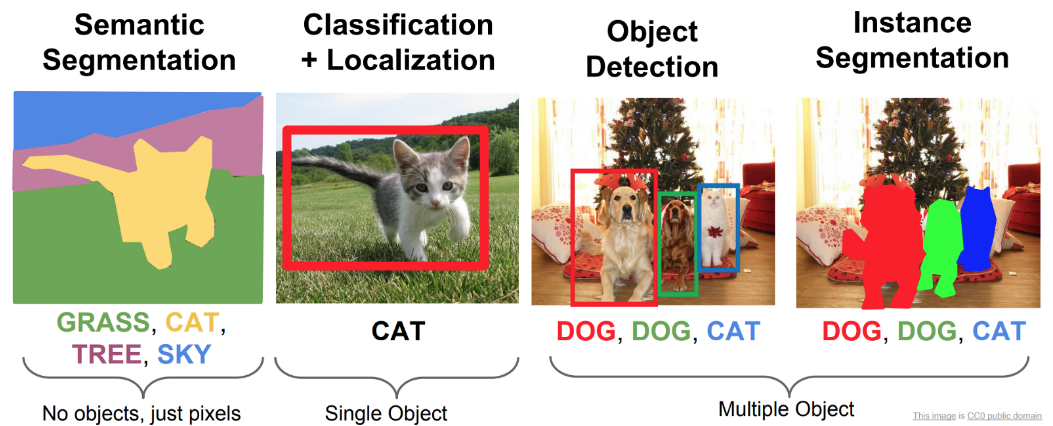
\includegraphics[height=0.35\textheight]{figures/applications/image_tasks.png}
%\end{center}
%\vsp
%\begin{center}
%    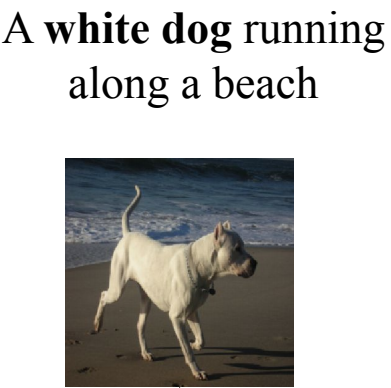
\includegraphics[height=0.3\textheight]{figures/applications/image_cap.png}
%\end{center}
%\vspace{8mm}
%\end{minipage}
%\hspace{5mm}
% {\footnotesize Images taken from \citem{nikolaus-etal-2019-compositional, ZhuPIE17, stanford2017}.}

\end{frame}

\begin{frame}{Deep learning: impact on \\wide range of applications (cont'd)}

\emphbf{Natural language \& speech}
\begin{itemize}
\item Machine translation
\item Automatic speech recognition
\item Text to speech
\item Text prediction/Language modeling
\item Text classification, generation, summarization...
\item Sentiment analysis
\item Question answering
\end{itemize}
\hspace{-8mm}
\begin{minipage}{0.2\linewidth}
  \begin{center}
    
\includegraphics[height=0.3\textheight]{figures/applications/g-translate.png}
  \end{center}
\end{minipage}
\begin{minipage}{0.35\linewidth}
  \begin{center}
    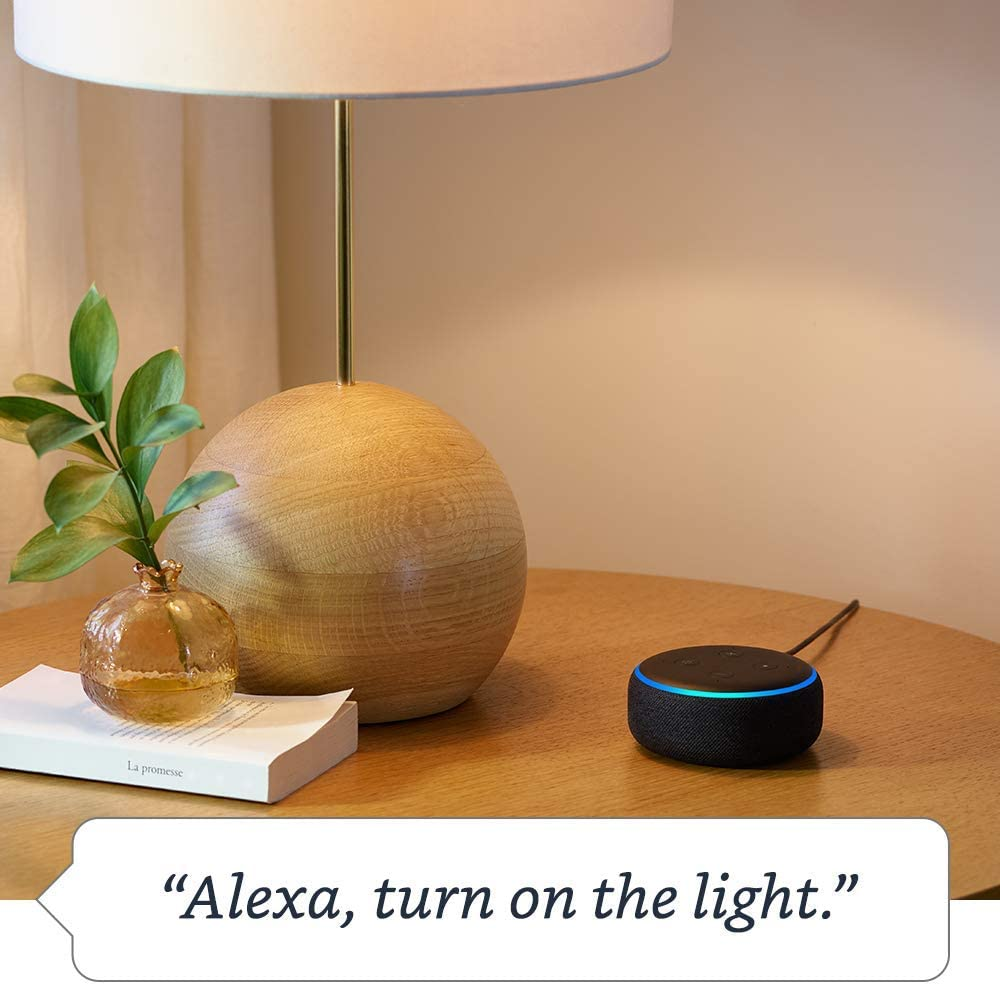
\includegraphics[height=0.4\textheight]{figures/applications/alexa.jpg}
  \end{center}
\end{minipage}
\begin{minipage}{0.35\linewidth}
  \begin{center}
    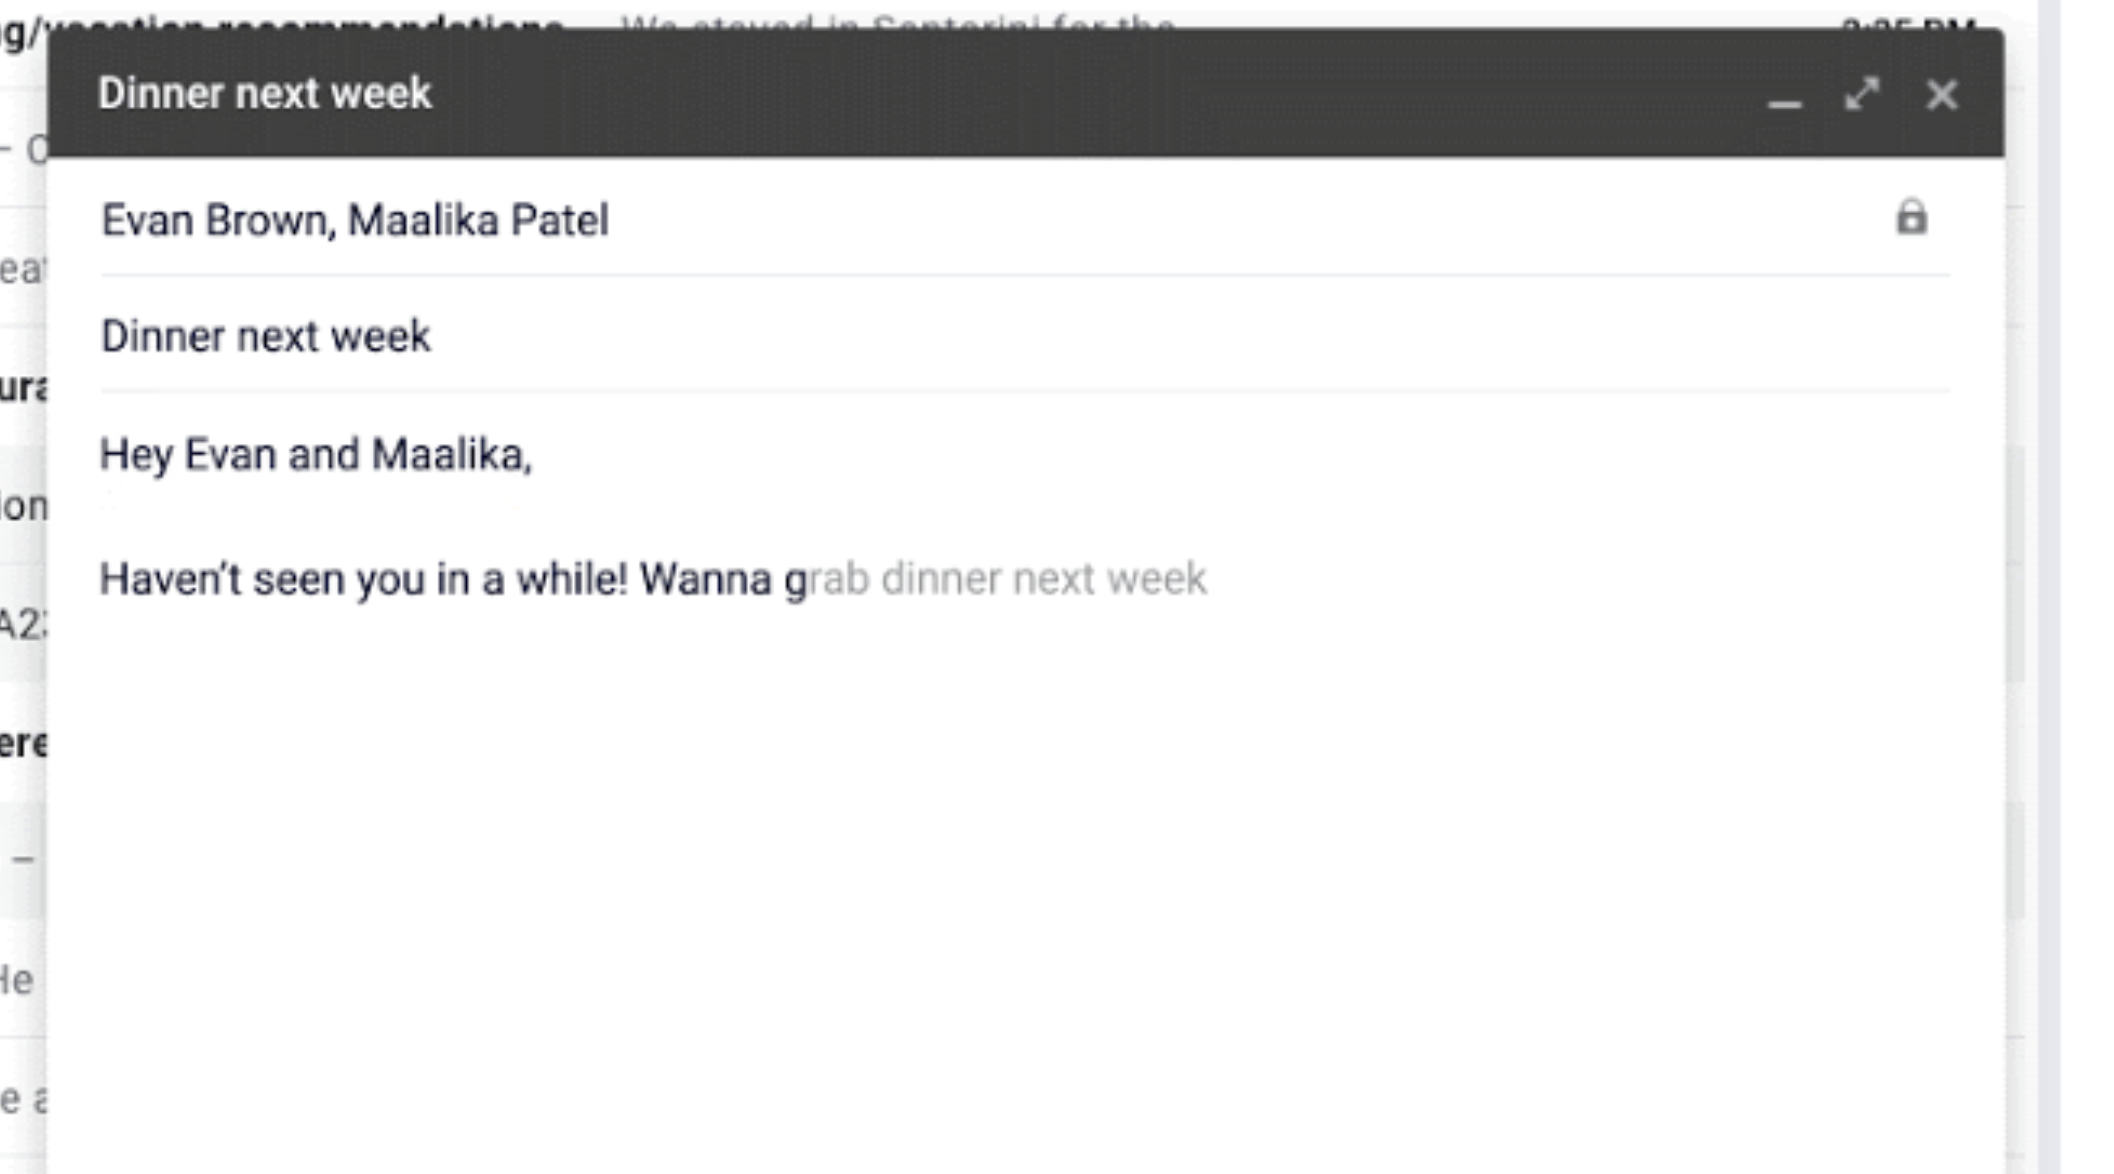
\includegraphics[height=0.5\textheight]{figures/applications/smart-compose.png}
  \end{center}
\end{minipage}
\end{frame}

\begin{frame}{Text generation (trending since 2019)}
%\begin{minipage}{0.45\textwidth}
\textbf{GPT} 2 \& 3 Language models (OpenAI, 2019/2020)
\begin{center}
    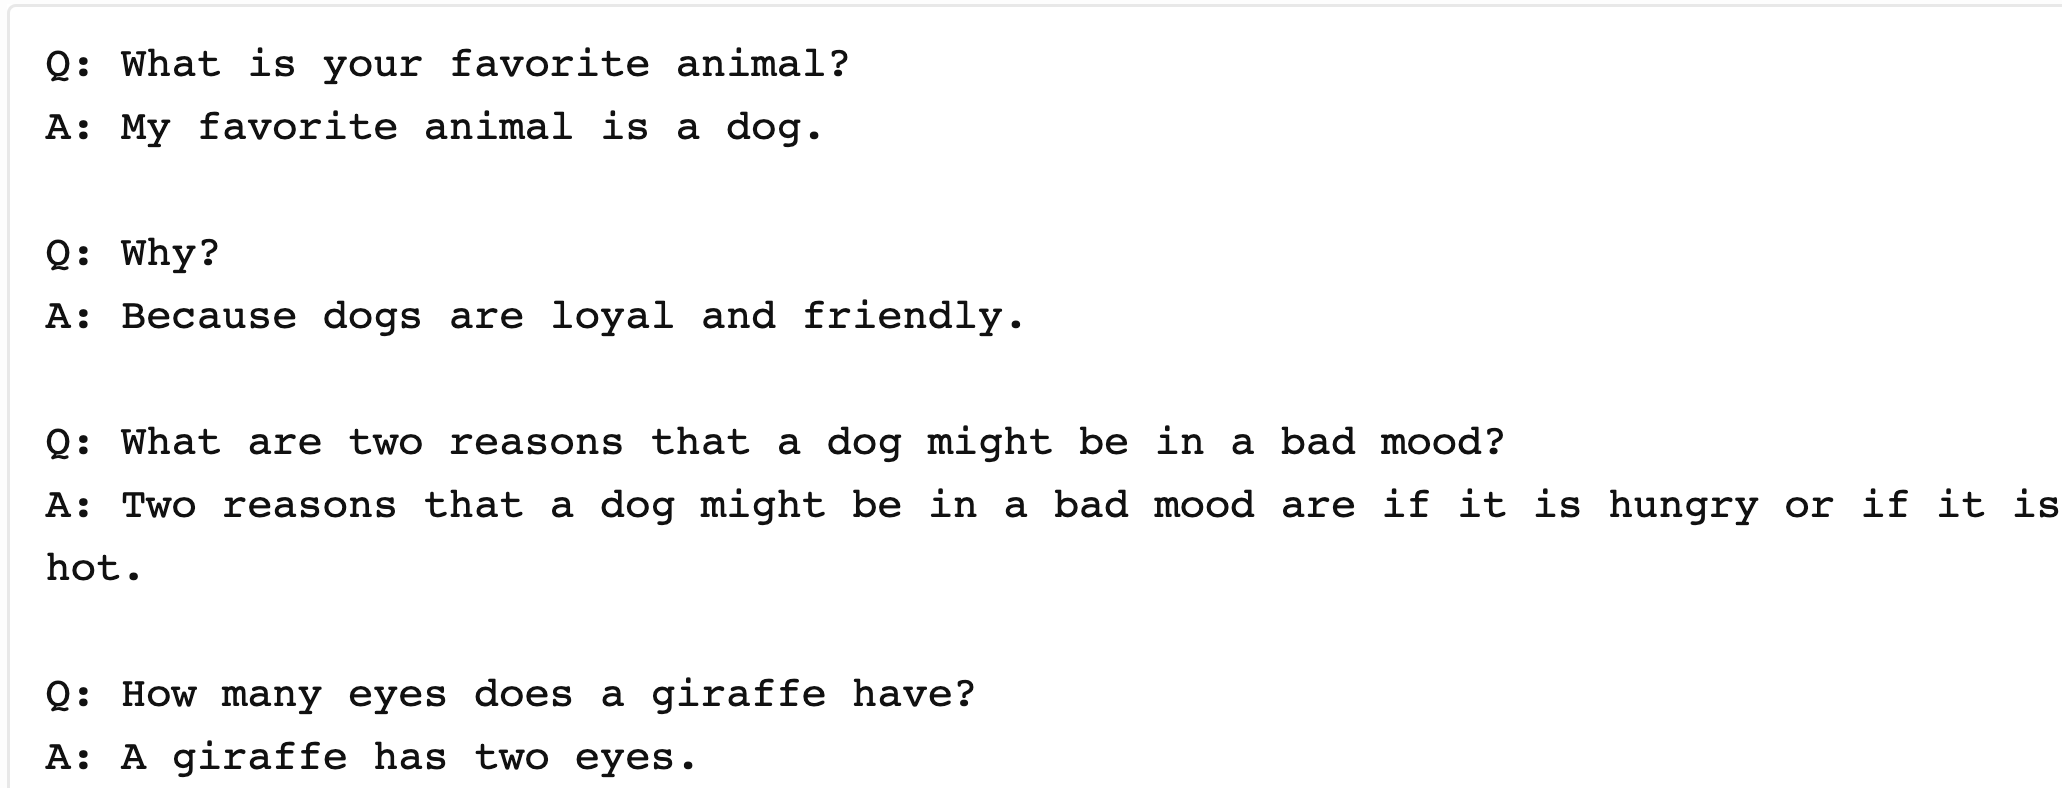
\includegraphics[height=0.6\textheight]{figures/applications/gpt_ex2.png}
\end{center}
{\small example taken from \link{https://lacker.io/ai/2020/07/06/giving-gpt-3-a-turing-test.html}}\\
Similar model applied to code generation: OpenAI Codex (2021) \\
Demo: \link{https://www.youtube.com/watch?v=SGUCcjHTmGY}

%\begin{minipage}{0.45\linewidth}
%\textbf{GPT} 2 \& 3(OpenAI, 2019/2020), text generation
%\begin{center}
%    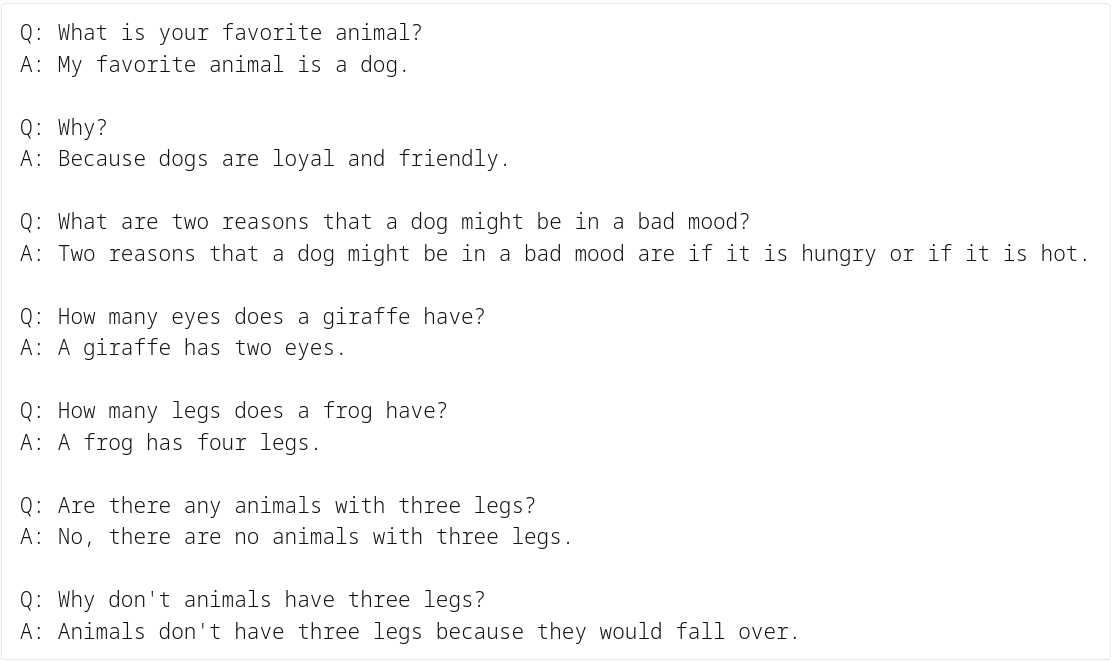
\includegraphics[height=0.5\textheight]{figures/gpt_3_output.png}
%\end{center}
%{\small example taken from \link{https://lacker.io/ai/2020/07/06/giving-gpt-3-a-turing-test.html}}
%\end{minipage}
%\vspace{3mm}
%\begin{minipage}{0.45\linewidth}
%OpenAI Codex (2021), natural language to code
%\begin{center}
%    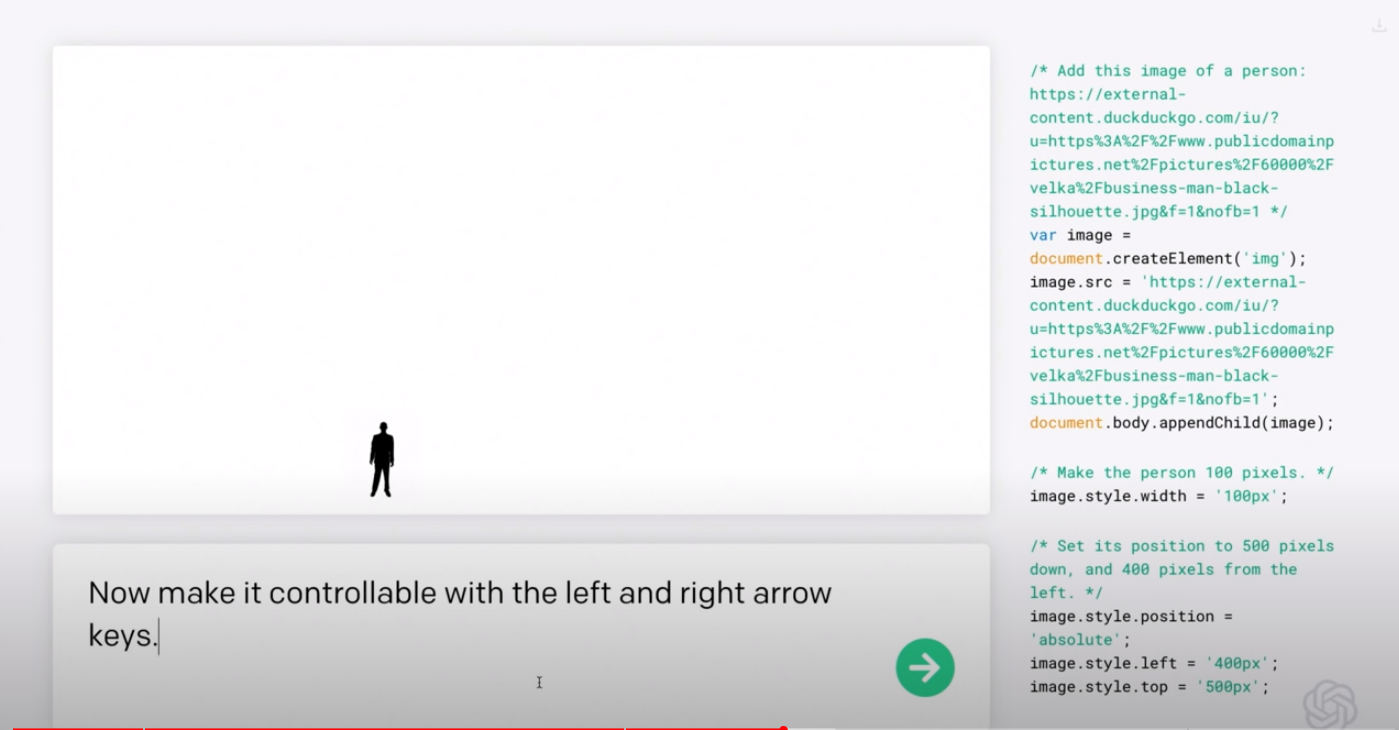
\includegraphics[height=0.3\textheight]{figures/codex_demo.png}
%\end{center}
%Demo: \link{https://www.youtube.com/watch?v=SGUCcjHTmGY}
%\end{minipage}
\end{frame}


\begin{frame}{Deep learning  applications:\\
many more domains...}
\begin{itemize}
\item Game playing (board/video games)
\item Robotics
\item Art and Music (generation)
\item Medical/pharmaceutical domain, drug discovery, chemical reaction prediction...
\item Financial engineering...
\end{itemize}
\vspace{3mm}
\begin{minipage}{0.3\linewidth}
  \begin{center}
    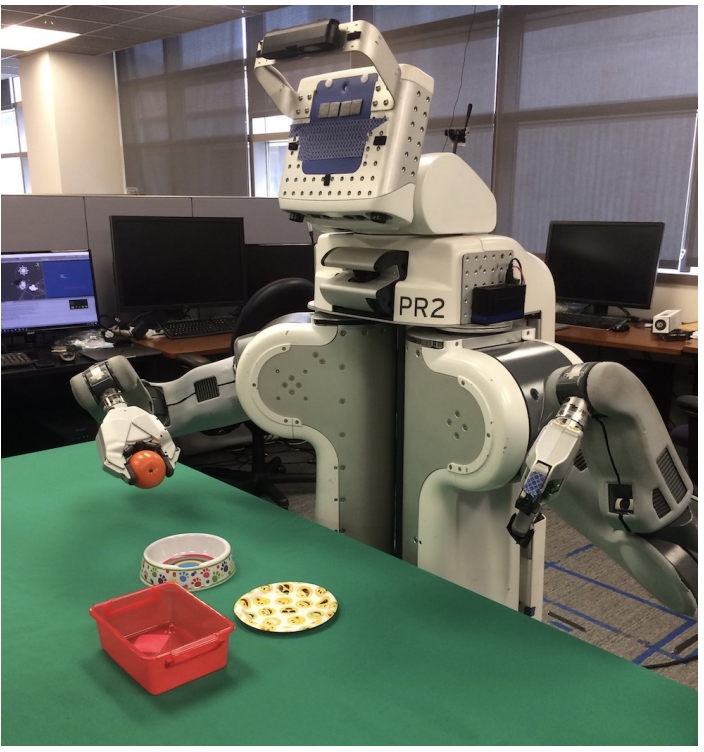
\includegraphics[height=0.5\textheight]{figures/applications/robot-manip.png}
  \end{center}
\end{minipage}
\begin{minipage}{0.25\linewidth}
  \begin{center}
    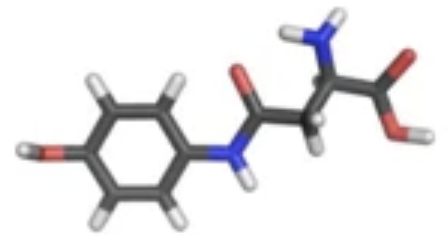
\includegraphics[height=0.2\textheight]{figures/applications/molecule.png}
  \end{center}
\end{minipage}
\begin{minipage}{0.4\linewidth}
  \begin{center}
    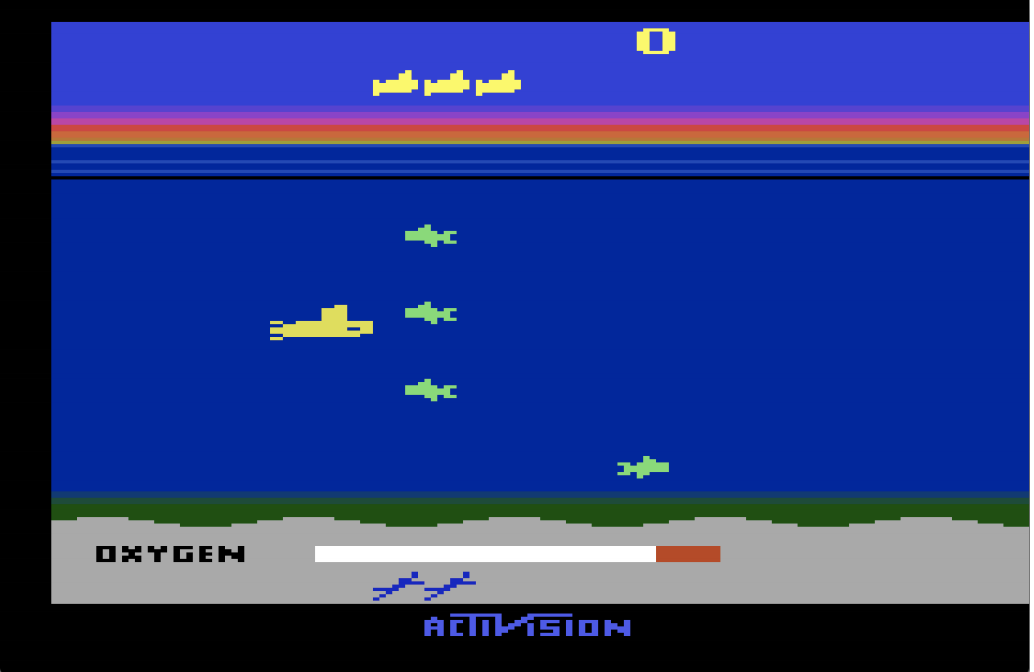
\includegraphics[height=0.4\textheight]{figures/applications/atari.png}
  \end{center}
\end{minipage}

\vspace{2mm}
{\small Figures taken from \citem{FinnYZAL17, kim2018deep, mnih-atari-2013}}
%Art/Music composition: 
%Games: video games, board games, chess, go...
%Robotics.
%OpenAI 
%Supervised learning, Reinforcement learning,...
%Also\\
%medical domain, finance...\\
\end{frame}

\begin{frame}{In this lecture...}
\vsp
\begin{itemize}
\item Unfortunately, we do not have enough time to cover everything...
\item But we'll study basic but fundamental tasks to illustrate various things that we can do with neural networks (the focus is on supervised learning).
\item Fundamental ideas are transferable to other tasks beyond in this course, and prepare you for future learning.
\item Application domains covered in the exercises:
\begin{itemize}
\item \textbf{Image classification} with feed-forward and \emphbf{convolutional neural networks}.
\item \textbf{Text generation} (and related tasks) with \emphbf{recurrent neural networks}.
\item \textbf{Mathematical problem solving} (and/or related translation-like tasks) with \emphbf{Transformers}.
\end{itemize}
\end{itemize}
%\vspace{3mm}
%\begin{minipage}{0.3\linewidth}
%  \begin{center}
%    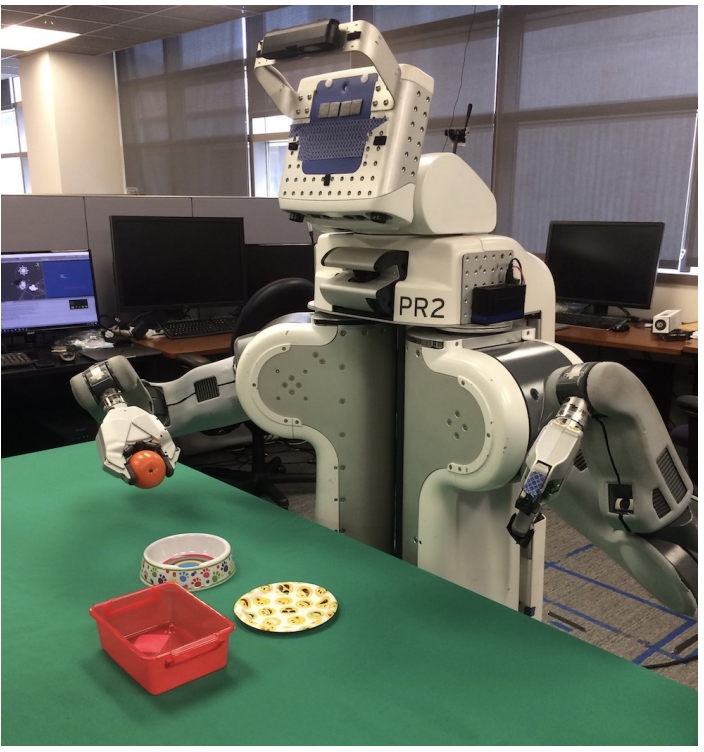
\includegraphics[height=0.5\textheight]{figures/applications/robot-manip.png}
%  \end{center}
%\end{minipage}
%\begin{minipage}{0.25\linewidth}
%  \begin{center}
%    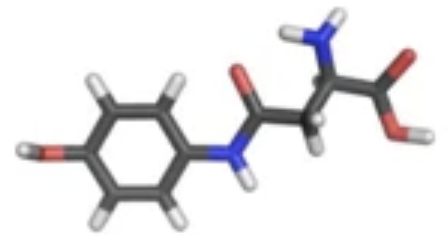
\includegraphics[height=0.2\textheight]{figures/applications/molecule.png}
%  \end{center}
%\end{minipage}
%\begin{minipage}{0.4\linewidth}
%  \begin{center}
%    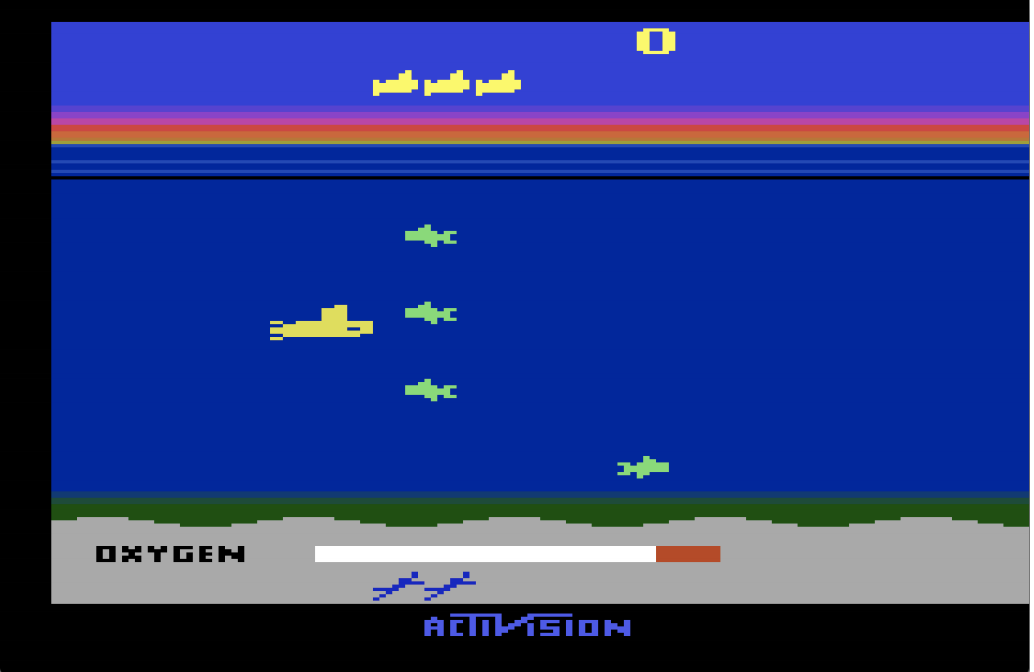
\includegraphics[height=0.4\textheight]{figures/applications/atari.png}
%  \end{center}
%\end{minipage}
%
%\vspace{2mm}
%{\small Figures taken from \citem{FinnYZAL17, kim2018deep, mnih-atari-2013}}
\end{frame}

%%%%%%%%%%%%%%%%%%%%%%%%%%%%%%%%%%%%%%%%%%%%%%%%%%%%%%%%%%%%%%%%%%%%%%%%%%

%\end{document}

%%%%%%%%%%%%%%%%%%%%%%%%%%%%%%%%%%%%%%%%%%%%%%%%%%%%%%%%%%%%%%%%%%%%%%%%%%


\tableofcontents[]  % shows the outline.

\section{Workflow Overview}

\begin{frame}{Introduction}
%\begin{itemize}[<+>]
\begin{itemize}
\item High-level principle:
\begin{itemize}
\item[-] data: many input/output example pairs.
\item[-] models \textbf{learn from examples}.
\end{itemize}
 \pause
\item For example:
\begin{itemize}
\item[-] You will \alertbf{not} write a hard-coded program which translates a English sentence to a French sentence.
 \pause
\item[-] Instead: you will \textbf{train} your \textbf{model/neural network} by letting it see many (many!) examples of paired English-French sentences (\textbf{training data}).
\end{itemize}
 \pause
\item Your model has \emphbf{parameters}, which are initially random.\\
\begin{itemize}
\item[-] \textbf{Training will modify/optimize the model parameters} such that they would minimize a \textbf{loss function} (correlated to the task you want to solve).
\end{itemize}
\pause
\item Your model and training setup have \emphbf{hyper-parameters}:
\begin{itemize}
\item[-] You train multiple models with different hyper-parameters and select the best model based on its \textbf{validation data} performance.
\end{itemize}
 \pause
\item The final model is evaluated on the \textbf{test data}.
%; in the example of translation, sentences unseen during the training.
\end{itemize}
\end{frame}

\begin{frame}{Typical Deep Learning Workflow\\ (supervised learning)}
\begin{itemize}
\item Define/obtain: \textbf{task, dataset}
\item Define \textbf{model}
\item Define \textbf{loss} and \textbf{optimization algorithm}
\item Do \textbf{training} and \textbf{hyper-parameter tuning}
\item Evaluate its performance using an \textbf{evaluation metric(s)}\\
(:= make prediction on the test data using the trained model; requires some search algorithm depending on the task)
\end{itemize}
\end{frame}

\begin{frame}{Task and Data}
Image classification? Speech recognition? Image question answering?\\
\vspace{5mm}
\textbf{For any problem,}
you should know your \textbf{\alert{task}} and \textbf{\alert{dataset}}:
\begin{itemize}
\item What are the \textbf{inputs \& outputs} to the system?
\item What are the \textbf{basic statistics} of the data?\\
 (size of the data, number of output classes, ...)
\item Which metric do you use to \textbf{evaluate} the final model performance?
\end{itemize}
\vspace{2mm}
General recommendation: take some time looking into data examples,
before building a model.
\end{frame}

\begin{frame}{Task and Data (cont'd)}
\textbf{Example 1:}
\vsp
\begin{itemize}
\item Task: \textbf{Image classification}
\pause
\item Nature of the problem: input = image, output = class label.
\pause
\item Dataset statistics? For example:
\begin{itemize}
\item[-] Number of training samples: 10K 100K? 1M? images (is this big? toy task?)
\item[-] Number of classes: 10? 100? 1000? classes (dog, cat, airplane,...)\\ (is this big? small/toy task?)\\
\end{itemize}
\pause
%Classifying between just dog and cat is different from classification among 1000 classes.
\item Evaluation metric: classification error or accuracy (number of correctly classified test images divided by the total number of test images).
\item Extra aspect: is this a standard benchmark dataset? do people publish on this dataset? What are the baseline models/performance? 
\end{itemize}
\end{frame}

\begin{frame}{Task and Data (cont'd)}
\textbf{Example 2:}
\vsp
\begin{itemize}
\item Task: \textbf{Machine Translation}
\pause
\item Nature of the problem:\\ input = text in the source language, output = text in the target language.\\
Each example: bilingual sentence pair.
\pause
\item Dataset statistics? For example: 
\begin{itemize}
\item Number of training sample:\\ 100\,M bilingual training sentence pairs (is this big? small/toy task?)
\item Vocabulary: word? sub-word? character? (choice for your system)
\item Vocabulary size: 30\,K in source and 40\,K tokens in target language.
\item (Domain of texts: News? European parlament?)
\end{itemize}
\item Evaluation measure: BLEU \citem{PapineniRWZ02}.
\end{itemize}
\end{frame}

\begin{frame}{Modeling}
\begin{itemize}
\item Architecture \& type of your model will depend on the task.\\
\item In particular: different input/output modalities.
\item \textbf{In Section 3}: different types of neural network architectures will be reviewed.
\item Here: quick reminder on basics of neural networks,\\
to introduce \textbf{key words} and practicalities.
\end{itemize}

\end{frame}

\begin{frame}{Modeling:\\Reminders on neural networks}
A Neural Network:
\begin{itemize}
\item is a \textbf{parameterized} function (whose parameters are \textit{learned} from data).\\
\pause
\item transforms a \textbf{vector to another vector} (the most standard case).\\
\pause
\item Such a layer can be composed multiple times (output of a layer becomes input to next layer...etc) to make the model \textbf{deeper}. \\Each layer with its own parameters (in principle).
\end{itemize}
\end{frame}


\begin{frame}{Modeling:\\Reminders on neural networks}
\textbf{Two basic operations.} Let $d_\text{in}$ and $d_\text{out}$ denote positive integers.

A typical \textbf{one-layer} feed-forward neural network transforms input $x\in\mathbb{R}^{d_\text{in}}$ to output $z\in\mathbb{R}^{d_\text{out}}$ as follows:
\begin{itemize}
\item \textbf{Affine transformation} (\emphbf{Linear layer}): $y = Wx + b$ where $W\in\mathbb{R}^{d_\text{out} \times d_\text{in}}$ is a \emphbf{weight matrix} and $b\in\mathbb{R}^{d_\text{out}}$ is a \emphbf{bias} vector.
$y\in\mathbb{R}^{d_\text{out}}$.\\
$W$ and $b$ are \emphbf{trainable parameters}.
% Loosely this is often refer to as a \textit{linear layer}.
\begin{figure}
\centering
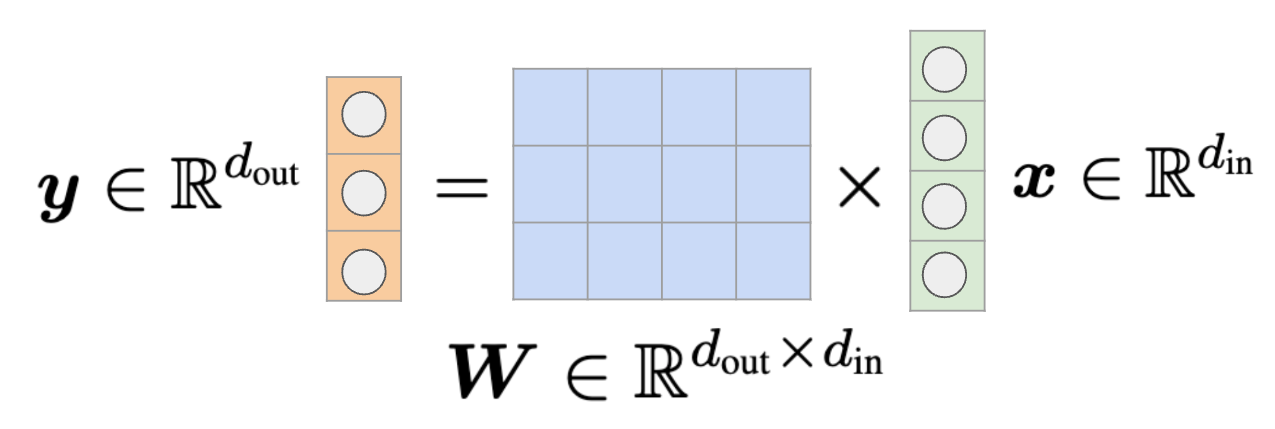
\includegraphics[width=0.80\linewidth]{./figures/linear.png}
\end{figure}
\pause
\item Element-wise non-linear \textbf{activation function}: $z = \sigma(y) \in\mathbb{R}^{d_\text{out}}$
\pause
\end{itemize}
We can compose many layers (an output of a layer becomes an input to the next layer...etc) to obtain a \emphbf{deep} neural net.
\end{frame}

\begin{frame}{Modeling:\\Reminders on neural networks (cont'd)}
\begin{minipage}{0.6\linewidth}
\textbf{Activation functions.}
\begin{itemize}
\item Commonly used functions:\\ \emphbf{sigmoid}, \emphbf{tanh},\\ rectifier linear unit (\emphbf{ReLU}).
\item More exotic functions:\\ ELU, GELU, SiLU...
\item For normalized output: \emphbf{softmax}.
\end{itemize}
\end{minipage}
\hspace{-8mm}
\begin{minipage}{0.38\linewidth}
\begin{figure}
                        \centering
                        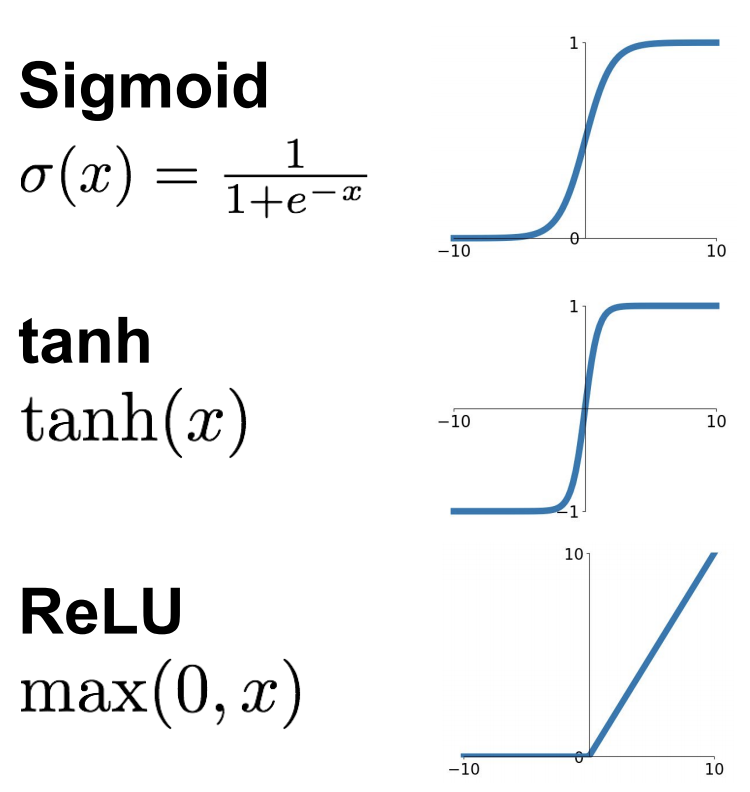
\includegraphics[width=0.95\linewidth]{./figures/activation.png}
\end{figure}
\tiny{Figure taken from \citem{stanford2019training}}
\end{minipage}
\end{frame}

\begin{frame}{Activation functions (cont'd)}
\textbf{Softmax function:}\\
\vsp
\begin{itemize}
\item[-] Let $d$ denote a positive integer
\item[-] Input $x\in\mathbb{R}^d$ is an arbitrary vector.
\item[-] Output $y\in\mathbb{R}^d$ defines a \emphbf{probability distribution}
\end{itemize}
% Input $x\in\mathbb{R}^n$, output $y\in\mathbb{R}^n$.\\
\vsp
For $1 \leq i \leq d$, $i$-th entry of vector $y\in\mathbb{R}^d$ is defined as: 
\[
 y_i = \displaystyle \dfrac{\exp(x_i)}{\displaystyle \sum_{n=1}^{d} \exp(x_n)}
\]
\vsp
The output vector $y$ has the following properties:
\begin{itemize}
\item All entries which are positive: For $1 \leq i \leq d$, $y_i > 0$.
\item The sum of all entries is one (normalized output): $\displaystyle \sum_{i=1}^{d} y_i = 1$.
\end{itemize}
The input $x$ to the softmax function is often called \emphbf{logit}.
\end{frame}

\begin{frame}{Model: illustration}
\begin{figure}
\centering
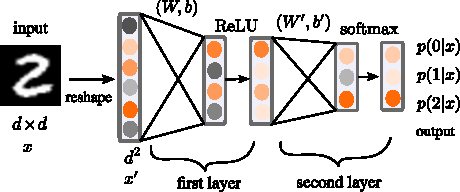
\includegraphics[width=0.90\linewidth]{./figures/nn_intro.pdf}
\end{figure}
\begin{itemize}
\item 2-layer feed-forward neural network model for\\
classification of $d$ by $d$ images of digits to 3 possible classes: 0, 1 or 2.
\end{itemize}
\end{frame}


% \begin{frame}{Modeling:\\Reminders (cont'd)}
% 
% Models have \emphbf{hyper-parameters} such as:
% \vsp
% \begin{itemize}
% \item Number of layers.
% \item Size of each hidden layer.
% \item ... other model specific hyper-parameters...
% \end{itemize}
% \vsp
% These hyper-parameters must be \emphbf{tuned}:
% \vsp
% \begin{itemize}
% \item Hyper-parameters are not \textit{learned} by the training algorithm!
% \item They are set before training and remain the same throughout training (with a few exceptions).
% \item Tuning: specify a set of hyper-parameters, train the model, and check its performance on some validation data, repeat until you obtain a "good" model.
% \item Tuning is a practice you learn from hands-on experience!
% \item We will come back to this in exercises.
% \end{itemize}
% \end{frame}

\begin{frame}{Training}
\textbf{Training}: optimization process to find the optimal values for the model parameters for the loss function.
\begin{itemize}
\item Before training: model parameters are random. 
\item After training: model parameters should have values which allow the model to solve the task!
\end{itemize}
\vsp
For that we must define:
\begin{itemize}
\item \textbf{Loss function}: function of model parameters to be minimized during training.
\item \textbf{Optimizer}:
specification of optimization algorithm with its hyper-parameters.
\end{itemize}
\vsp
\emphbf{Training hyper-parameters} need to be tuned: e.g. learning rate...
\end{frame}

\begin{frame}{Training: Loss}
\begin{itemize}
\item Let $N$ and $P$ denote positive integers.\\
A super script $i$ in $x^i$ denotes $i$-th training example.
\item \emphbf{Training data} $\{(x^1, y^1), ..., (x^N, y^N)\}$\\
is a set of $N$ input $x^i$ and output/target $y^i$ pairs.
\item[-] The exact specification of the nature of $x^i$ and $y^i$ does not matter here (you can assume that they are both vectors).
\pause
\item We want to train our \emphbf{model} $f_{\theta}$ with $P$ trainable \emphbf{parameters} $\theta \in \mathbb{R}^P$.
\item[-] \emphbf{Loss function} $\displaystyle \mathcal{L(\theta)} = \dfrac{1}{N} \sum_{i=1}^N \ell\left(f_{\theta}(x^i), y^i\right)$\\
with some function $\ell$ (dependent of the problem) which ``\textit{compares}'' each model output/prediction $f_{\theta}(x^i)$ and the target (true label) $y^i$.
% \item Typical notation: ``hat'' for the model prediction:  $\hat{y}^i = f_{\theta}(x^i)$
\end{itemize}
\end{frame}

\begin{frame}{Training: Loss (cont'd), Reminders}
\vspace{-5mm}
% Reminders:
% \vsp
For \textbf{regression} problems, let $d$ denote a positive integer (target vector size)
\begin{itemize}
\item Target $y^i  \in \mathbb{R}^d$ is a \textbf{vector}
\item so is the model output $f_{\theta}(x^i) \in \mathbb{R}^d$.\\
\vsp
\end{itemize}
Using the squared error
$\ell\left(f_{\theta}(x^i), y^i\right) = \|f_{\theta}(x^i) - y^i  \|^2_2$ we get the\\
\emphbf{Mean Squared Error (MSE) Loss}: $\displaystyle \mathcal{L(\theta)} = \dfrac{1}{N} \sum_{i=1}^N \|f_{\theta}(x^i) - y^i  \|_2^2$
\end{frame}

\begin{frame}{Training: Loss (cont'd), Reminders}
\vspace{-5mm}
% Reminders:
% \vsp
For \textbf{classification} problems, let $C$ denote a positive integer (number of output classes).
\begin{itemize}
\item Target $y^i  \in \{1...C\}$ is a  \textbf{label}/integer
\item Model output $f_{\theta}(x^i) \in \mathbb{R}^C$ is a vector defining a \textbf{probability over the class labels}:\\
$f_{\theta}(x^i)= \left[p_{\theta}(1|x^i),... , p_{\theta}(k|x^i),.. ,p_{\theta}(C|x^i)\right]$ for $k\in \{1...C\}$\\
where $p_{\theta}(k|x^i) \in \mathbb{R}$ is a probability that the input is of class $k$ according to the model.\\
\end{itemize}
\vsp
Using cross entropy (where $\delta_{y^i, k} = 1$ if $y^i=k$, $0$ otherwise) $\displaystyle \ell\left(f_{\theta}(x^i), y^i\right) = - \sum_{k=1}^C \delta_{y^i, k} \log p_{\theta}(k|x^i) = - \log p_{\theta}(y^i|x^i)$ \hspace{1mm} we get the\\
\emphbf{Cross-Entropy Loss}: $\displaystyle \mathcal{L(\theta)} = -\dfrac{1}{N} \sum_{i=1}^N \log p_{\theta}(y^i|x^i)$
\end{frame}

\begin{frame}{Training: Optimization/mini-batch}
Having defined the loss function $\displaystyle \mathcal{L(\theta)} = \dfrac{1}{N} \sum_{i=1}^N \ell\left(f_{\theta}(x^i), y^i\right)$\\
\vsp
\textbf{Gradient descent:}
\begin{itemize}
\item is an iterative process. At iteration step $n$, update $\theta(n) \in \mathbb{R}^P$ to $\theta(n+1) \in \mathbb{R}^P$ by
\item[-] computating gradients $\nabla_{\theta}\mathcal{L}(\theta(n)) \in \mathbb{R}^P$ (e.g., by \textbf{backpropagation}).
\item[-] applying one gradient descent step: $\theta(n+1) = \theta(n) - \alpha * \nabla_{\theta} \mathcal{L}(\theta(n))$\\
where $\alpha \in \mathbb{R}_{+}$ is \emphbf{learning rate} (hyper-parameter!)
\pause
\item This is repeated multiple times (needs to define some stopping criterion)
\pause
\item \textbf{Gradients computed on the whole dataset (average over $N$) for each update. Inefficient?}
\end{itemize}
\pause
\vsp
\textbf{Alternative: update parameters using gradients computed on} \emphbf{mini-batches}
% \emphbf{stochastic gradient descent (SGD)}.
\begin{itemize}
\item Gradients computed on a few, randomly selected data points (mini-batch or simply \textit{batch})
\item Number of data points in a batch is the \emphbf{batch size} (also hyper-parameter)!
\item Allows more frequent updates (works well in practice)
\end{itemize}
%\vsp
%\pause
%Many variants: Adam, Adadelta, Adagrad etc...\\
%Motivation: adaptive learning rates for each parameter.
% learning rate scheduling...
%If you are interested in Optimization in general:
%\link{https://web.stanford.edu/~boyd/cvxbook/bv_cvxbook.pdf}
\end{frame}


\begin{frame}{Note: parallel computation\\ e.g. processing $N$ inputs to a linear layer}
\begin{figure}
\centering
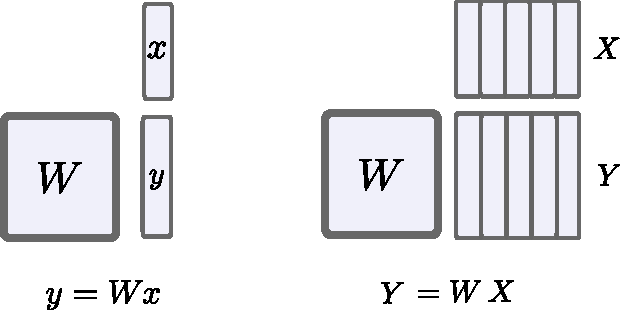
\includegraphics[width=0.80\linewidth]{./figures/batch.pdf}
\end{figure}
$W \in \mathbb{R}^{d_\text{out} \times d_\text{in}}$, $y \in \mathbb{R}^{d_\text{out}}$ and $x \in \mathbb{R}^{d_\text{in}}$ \textbf{VS.}  $Y \in \mathbb{R}^{d_\text{out} \times N}$ and $X \in \mathbb{R}^{d_\text{in} \times N}$
\begin{itemize}
\item Computing linear transformation of \textbf{multiple examples} can be packed into a \textbf{single} matrix-matrix multiplication.
\item Benefit from efficient parallel computation (especially on GPUs).
\item Should write \textbf{vectorized code} instead of loop (example later)
\end{itemize}
\end{frame}


\begin{frame}{Training: Optimization/Optimizer}
\begin{itemize}
\item The parameter update equation in the previous slide:\\
$\theta(n+1) = \theta(n) - \alpha * \nabla_{\theta} \mathcal{L}(\theta(n))$\\
with gradients computed on a mini-batch corresponds to \emphbf{stochastic gradient descent (SGD)} algorithm.
\pause
\item[-] This makes use of the same learning rate $\alpha$ for all parameters.
\begin{itemize}
\item[-] Many other variants for optimization algorithm with adaptive learning rates for each parameter has been proposed.
Popular overview: \link{https://ruder.io/optimizing-gradient-descent/}
\end{itemize}
\pause
\item[-] \textit{adaptive}: change the effective learning rate depending on the past gradients of the corresponding parameter.
\begin{itemize}
\item[-] In particular, \textit{Adam} \citem{kingma15} is very popular.
\end{itemize}
\pause
\item \textbf{Choosing an optimizer = specifying the choice of optimization algorithm and its hyper-parameters.}
\item[-] Hands-on experience in exercises.
\end{itemize}
\end{frame}


\begin{frame}{Some Training Jargon}
\textbf{Progress of training} is often discribed in terms of number of:
\vsp
\begin{itemize}
\item \emphbf{Epochs}: 1 epoch = one run over the whole training data.
\item \emphbf{Steps}: 1 step = 1 gradient update (typically using 1 mini-batch).
\item \emphbf{Updates}: normally synonym to steps.
\item More rarely, \emphbf{sub-epochs}: some fixed fraction of epoch,\\ e.g. 1/4 of epoch.
\end{itemize}
\vsp
The descriptions above are typically correct.\\
But unconventional definitions can also be found in some papers...
\end{frame}

\begin{frame}{Hyper-Parameter Tuning}
 Models have \emphbf{hyper-parameters} such as:
 \begin{itemize}
 \item[-] Number of layers, size of each hidden layer, other model specific hyper-parameters...
 \end{itemize}
\pause
\vsp
So do training algorithms:
 \begin{itemize}
 \item[-] Learning rate, batch size, other optimizer specific hyper-parameters...
 \end{itemize}
\pause
\vsp
Hyper-parameters are not \textit{learned} by the training algorithm!
 \begin{itemize}
% \item They are set before training and remain the same throughout training (with a few exceptions).
 \item \textbf{Tuning}: specify a set of hyper-parameters, train the model, and check its performance on validation data, repeat until you obtain a "good" model.
\item Important, because: \emphbf{model performance can highly depend on the hyper-parameter tuning!}
 \item Tuning is a practice you learn from hands-on experience.
% \item We will come back to this in exercises.
 \end{itemize}

%\begin{itemize}
%\item Both \textbf{model} and \textbf{training algorithm} have hyper-parameters.
%\item They can be \textit{tuned} by looking at model performance on \textbf{validation/development set}.
%\item Important, because: model performance \alertbf{highly depends on the hyper-parameter tuning!}\\
%\item Need to learn to make things to work!
%\end{itemize}
%\vsp
%Illustrated in the exercises.
\end{frame}

\begin{frame}{Summary}
\textbf{What have we learned?}
\begin{itemize}
\item Overview of workflow: main concepts, key words.
\begin{itemize}
\item task \& data, nature of the problem, statistics.
\item evaluation measure
\item model
\item training
\item loss function
\item stochastic gradient descent
\item hyper-parameter tuning
\end{itemize}
\end{itemize}
\vsp
\textbf{Coming up next...}
\begin{itemize}
\item How can we implement these concepts concretely?
\item Introduction to tools for that.
\item ...
\end{itemize}
\end{frame}


% \tableofcontents[]  % shows the outline.
\section{Introduction to Tools}
% -----------------------------------------------------------------------
\subsection{Basic Tools}
\begin{frame}{Tools?}
\begin{itemize}
\item \emphbf{Practical implementation} implies a number of \emphbf{choices} in terms of framework or software to use.
For example:
\item Programming language: Python
\item Deep learning library: PyTorch
\item and more...
\item This section: introduction to these practical \textit{tools}.
\end{itemize}
% PyCharm: demo. Very convenient for both reading and writing!
\end{frame}

\begin{frame}{Python}
\begin{itemize}
\item Again: if you are not familiar with Python, check: \link{https://docs.python.org/3/tutorial/}
\item High-level, general purpose, programming language
\begin{itemize}
\item[-] ``easy to use", "broadly popular"
\item[-] The most popular language for deep learning today
\item[-] Many libraries are available.
\item[-] A few characteristics:\\ \textit{indentation} is part of syntax, dynamically typed, indices start from 0... etc
\end{itemize}
\item \alertbf{Version} to be used: Python 3.6+.
\item You will still find Python 2.x code... \\
But for any new code use: Python 3.6+.
\end{itemize}
% PyCharm: demo. Very convenient for both reading and writing!
\end{frame}

\begin{frame}[fragile]{Python, simple illustration}
\vspace{-5mm}
%Bubble sort\footnote{taken from {\scriptsize \url{https://realpython.com/sorting-algorithms-python/}}}:
\begin{python}
def bubble_sort(list_nums):
    # Implement Bubble Sort.
    already_sorted = True
    numbers = list_nums.copy()
    n = len(numbers)
    for i in range(n):
        for j in range(n-i-1):
            if numbers[j] > numbers[j+1]:
                numbers[j], numbers[j+1] = numbers[j+1], numbers[j]
                already_sorted = False
        if already_sorted:
            break
    return numbers
\end{python}
\pause
\begin{python}
>>> my_numbers = [58, 37, 2, 11, 96, 15, 64]
>>> bubble_sort(my_numbers)
[2, 11, 15, 37, 58, 64, 96]
\end{python}
\pause
Though you should use \textbf{built-in} function instead (more efficient).
\begin{python}
>>> sorted(my_numbers)
[2, 11, 15, 37, 58, 64, 96]
\end{python}
\end{frame}

\begin{frame}[fragile]{Python, simple illustration 2}
\vspace{-5mm}
\textbf{Loops} in Python are very simple (check Sec.~5.6 in the tutorial)
\begin{python}
# dictionary storing count of fruits.
>>> basket = {'apple': 4, 'banana': 2, 'orange': 5}
>>> for fruit, count in basket.items():
...   print(fruit, count)
... 
apple 4
banana 2
orange 5
\end{python}
\pause
\begin{python}
# loop over a list, with loop counter:
>>> for i, v in enumerate(['tic', 'tac', 'toe']):
...     print(i, v)
...
0 tic
1 tac
2 toe
\end{python}
\end{frame}

\begin{frame}[fragile]{Python, many packages}
\vspace{-3mm}
\textbf{Different packages} provide you with useful functions.\\
\vsp
E.g. \code{math} module for quick calculations:
(e.g. you want to immediately know the log of some number!)
\begin{python}
>>> import math
>>> math.log(0.1)
-2.3025850929940455
>>> y = math.log(0.1)
>>> z = math.exp(y)
>>> z
0.10000000000000002
\end{python}
\begin{itemize}
\item \textbf{NumPy} \code{numpy}: manipulation of multi-dimensional arrays.\\
\begin{itemize}
\item Seen in \emphbf{Exercise 1} !
\end{itemize}
\item \textbf{Matplotlib} \code{matplotlib}: tool for visualization, generate plots.
\begin{itemize}
\item More in \emphbf{Exercise 2} !
\end{itemize}
\item etc...
\end{itemize}
\end{frame}

\begin{frame}[fragile]{Python, package installer}
\vspace{-3mm}
The basic \textbf{package installer} for Python is \code{pip} (or \code{pip3} or Python 3).\\
\vsp
\begin{itemize}
\item To install the latest version of ``SomeProject”:\\
\begin{python}
pip3 install "SomeProject"
\end{python}
\item To install a specific version (e.g. version 1.1):\\
\begin{python}
pip3 install "SomeProject==1.1"
\end{python}
\end{itemize}
%Alternatively: If you can use \textbf{Anaconda/Miniconda}, see e.g.:
%\link{https://docs.conda.io/projects/conda/en/latest/user-guide/concepts/installing-with-conda.html}\\
%(\code{conda} is very convenient for environment managing; see later slides).
\end{frame}

\begin{frame}{Code Style}
\vspace{-3mm}
\textbf{Need guidelines to write consistent (easy to read) code.}
\begin{itemize}
\item How should I name my function? my variable? class?
\item How should I space? indent? comment?
\item What is the longest acceptable line length?\\
\item How to split long lines... etc!
\end{itemize}
\vsp
\textbf{Some reference guidelines:}\\
\begin{itemize}
\item PEP 8
\link{https://www.python.org/dev/peps/pep-0008/}
\item Google guideline
\link{https://github.com/google/styleguide/blob/gh-pages/pyguide.md}
\end{itemize}
\vsp
\textbf{Crucial importance for collaborative projects!}\\
\begin{itemize}
\item When you ask other people to \textbf{review} your code.
\item But also for yourself (to ease reading your own code).\\
\item \emphbf{Consistent} formatting makes reading much easier.
\end{itemize}
\end{frame}

\begin{frame}{Editor (for Python)}
\textbf{Up to you!}
\begin{itemize}
\item Emacs, vim, nano, kate, VSCode, ...\\
\item If you do not know, you can try \textbf{VSCode} or \textbf{PyCharm} (Community).
\begin{itemize}
\item Very convenient for both reading (navigating through a large project) and writing (with less formatting errors).
\end{itemize}
\item What I use: vim (for simple edits) and VSCode in general.
\end{itemize}
\end{frame}

\begin{frame}{Managing environment}
\textbf{(Excursion; no need to worry about this in this course)}
\vsp
\begin{itemize}
\item Python, libraries, softwares, ... evolve over time.
\item Resulting in code with \emphbf{different versions} for each tool.
\begin{itemize}
\item[-] Currently working code has no guarantee to work again in another environment.\\
\item[-] Also: often you will be using code that you find on the internet (Github), that someone had written, you do not know when, which requires some specific sets of versions for libraries...
\end{itemize}
%\item You might need to create a specific set of these packages
%in order to be able to run many different code/software.
%demo.
\end{itemize}
\vsp
\emphbf{Environment managing tools} can help handling multiple configurations.
\begin{itemize}
\item Typical tools: \code{virtualenv}, \code{conda}
\item If you do not have any preference yet, try Miniconda.\\
\begin{itemize}
\item[-] \link{https://docs.conda.io/en/latest/miniconda.html}
\item[-] \link{https://docs.conda.io/projects/conda/en/latest/user-guide/tasks/manage-environments.html}
\end{itemize}
\end{itemize}
% Example: \codeb{conda activate DL-lab} in your ICS script.
\end{frame}

%\begin{frame}{Managing environment (cont'd)}
%\begin{itemize}
%\item Basically: you want to maintain multiple sets of packages with their correct versions.\\
%\item Typical tools: \code{virtualenv}, \code{conda}
%\item If you do not have any preference yet, try Miniconda.
%\begin{itemize}
%\item \link{https://docs.conda.io/en/latest/miniconda.html}
%\item \link{https://docs.conda.io/projects/conda/en/latest/user-guide/tasks/manage-environments.html}
%\end{itemize}
%\end{itemize}
%\emphbf{demo?}
%\end{frame}

\begin{frame}{Other useful tools}
\begin{itemize}
\item Internet and Google!
\item Very likely, the same problem you encountered has been already solved by other people!
\item Search your problem, and you might find solutions on e.g. \textit{StackOverflow}.
\item Be careful with version mismatch.
\end{itemize}
\end{frame}

\begin{frame}{Libraries for Deep Learning}
\vspace{-3mm}
\textbf{Many possibilities, different teams/companies.}
\begin{itemize}
\item TensorFlow (Google), MXnet (Amazon), JAX (Google),...
\item Other high-level framework: keras (Google), ...
\end{itemize}
\pause
\vsp
\textbf{Side notes:}
\begin{itemize}
\item Theano (UdeM): end of support in 2017.
\item Chainer (Preferred Networks): migration to PyTorch in 2019.
\item Caffee (Berkeley, Facebook) merged to PyTorch in 2018. 
\item Cognitive Toolkit (Microsoft): 2016-2017.
\item even older... Quicknet (Berkeley)
\end{itemize}
\pause
\vsp
This lecture: \textbf{PyTorch}
\begin{itemize}
\item Development led by Meta/Facebook AI Research.
\item Last week: became a project under Linux Foundation
\item Very popular already. Increasing popularity...
\item Used for example by OpenAI, Tesla...
\end{itemize}
\end{frame}
% \subsection{Introduction to PyTorch}

\begin{frame}[fragile]{Introduction to PyTorch}

\textbf{Two core aspects:}
\vsp
\begin{itemize}
\item GPU-friendly tensors.
\item Automatic differentiation.
\end{itemize}
\vsp
Note: current version PyTorch 1.12.1 (Aug. 2022) \sout{PyTorch 1.9.0 (June 2021)} \sout{PyTorch 1.6.0 (July 2020)} \\
%\begin{python}
%import torch
%\end{python}
\end{frame}

\begin{frame}{Introduction to PyTorch (cont'd)}
\textbf{Packages which you will be often importing:}\\
\begin{itemize}
\item \codeb{torch}: top-level package.
\item \codeb{torch.nn}: modules for building neural networks. 
\item \codeb{torch.nn.functional}: various functions.
\item \codeb{torch.optim}: optimization related tools. 
\item \codeb{torch.utils}: handling data etc.
\item ...
\end{itemize}
Many examples later.
\end{frame}

% \subsection{Introduction to PyTorch}
\begin{frame}{Introduction to PyTorch (cont'd)}
\textbf{Many packages are available.}\\
\vsp
E.g.~to work with:
\begin{itemize}
\item image: \codeb{torchvision}
\item audio: \codeb{torchaudio}
\item text: \codeb{torchtext}
\item ...
\end{itemize}
\vsp
\end{frame}

\begin{frame}{Tensors}
\pause
\textbf{These are all tensors.}
\vspace{5mm}
  \begin{center}
    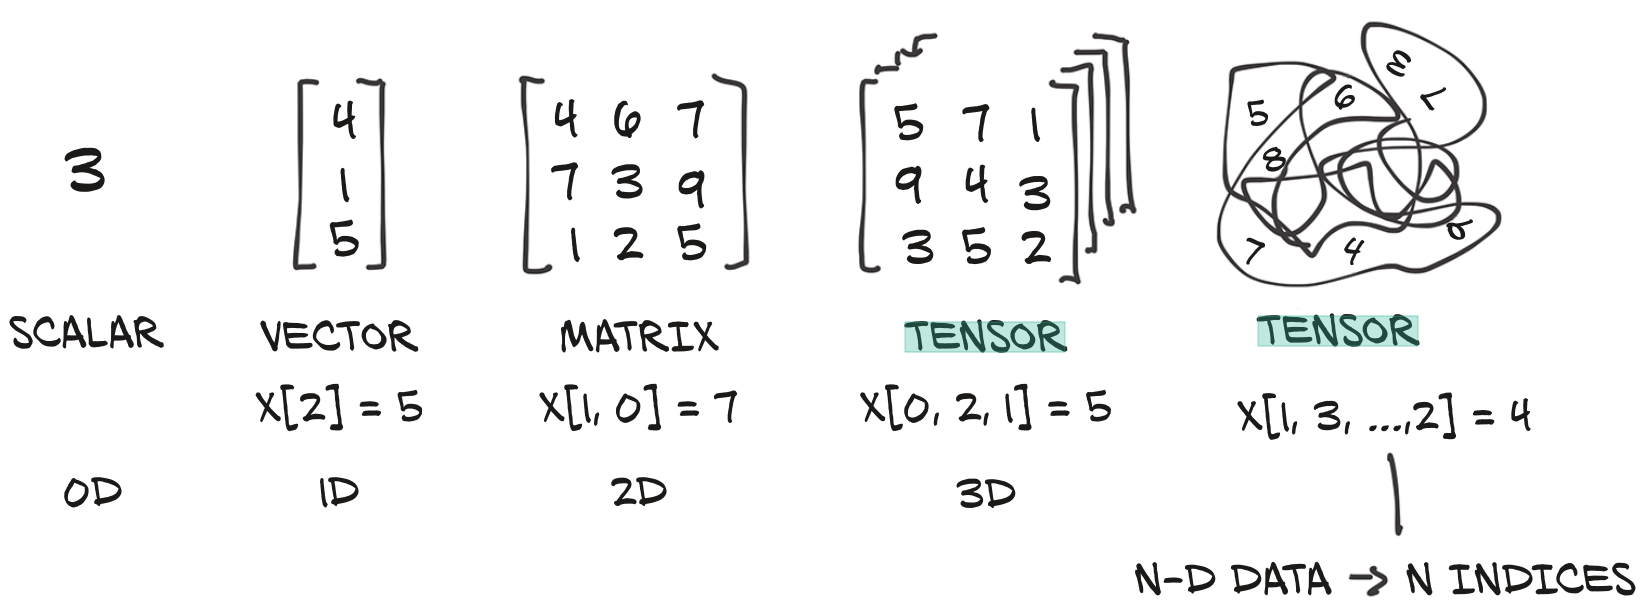
\includegraphics[height=0.5\textheight]{figures/tensors.png}
  \end{center}
\textbf{Including those with a rank of 0, 1 and 2, which have common names:\\ scalar, vector, matrix.}\\
\vspace{5mm}
\scriptsize{Figure taken from \citem{pytorchbook2020}.}\\
\end{frame}

\begin{frame}{Tensors (cont'd)}
\textbf{You will be manipulating multi-dimensional arrays all the time:}
\vsp
\begin{itemize}
\item You have an image.\\ It has height, width, and color channels (each pixel represented by red-green-blue): it's a 3d-array.\\ You have multiple images: you get a 4d-array.
\pause
\item You have a written sentence. \\You replace each word in the sentence by its ID, you get a 1d-array.\\ You have multiple sentences; you get a 2d-array.\\ (some subtlety w/ handling various sentence lengths)
\pause
\item These are all \emphbf{tensors}.
\end{itemize}
\vsp
Corresponding class in PyTorch is \codeb{torch.Tensor}.\\
Similar to NumPy's \codeb{numpy.ndarrays}.
\end{frame}

\begin{frame}[fragile]{Tensors, basic concepts}
\vspace{-7mm}
\codeb{torch.tensor} function creates \codeb{torch.Tensor} object:
\begin{python}
>>> import torch
>>> x = torch.tensor([[1, 2], [3, 4]])
>>> x
tensor([[1, 2],
        [3, 4]])
\end{python}
\pause
A fundamental attribute is the \emphbf{shape} of tensor:
\begin{python}
>>> x.shape  # or `x.size()`
torch.Size([2, 2])
\end{python}
\pause
Also: every \codeb{torch.Tensor} has \codeb{dtype} (data type) attribute.
\vspace{-1mm}
\begin{python}
>>> x.dtype
torch.int64
>>> x = torch.tensor([[1, 2], [3, 4]], dtype=torch.float32)
>>> x
tensor([[1., 2.],
        [3., 4.]])
>>> x.dtype
torch.float32
\end{python}
\end{frame}

\begin{frame}[fragile]{Tensors (cont'd)}
\vspace{-7mm}

You can create some classic/random tensors using e.g.
\begin{itemize}
\item  \codeb{eye} (diagonal tensor), \codeb{zeros} (all-zero tensor), \codeb{ones} (all-one tensor), \codeb{arange} (1D tensor with incrementally increasing integers),
\codeb{rand} (random tensor),... by specifying the shape/size you want.
\end{itemize}
\begin{python}
>>> x = torch.ones([2, 3])
>>> x
tensor([[1., 1., 1.],
        [1., 1., 1.]])
\end{python}
\begin{python}
>>> x = torch.rand([2, 3])
>>> x
tensor([[0.9332, 0.0222, 0.0364],
        [0.7155, 0.8362, 0.9795]])
\end{python}
\end{frame}

\begin{frame}[fragile]{Tensors, \\conversion from/to NumPy ndarrays.}
Simply: \codeb{torch.from\_numpy()} and \codeb{x.numpy()}
\begin{python}
>>> import numpy
>>> import torch
>>> a = numpy.array([1, 2, 3])
>>> a
array([1, 2, 3])
>>> b = torch.from_numpy(a)
>>> b
tensor([1, 2, 3])
>>> b.numpy()
array([1, 2, 3])
\end{python}

\end{frame}

\begin{frame}{Tensors,\\ manipulating dimensionality}
\textbf{Checking the shape of tensor:}
\begin{itemize}
\item \codeb{x.size()}  return tuple-like object of shape.
\item \codeb{x.shape}  same as above (alias).
\item \codeb{x.ndim}  return number of dimensions
\end{itemize}
\vsp
\pause
\textbf{Modifying the shape of tensor:}
\begin{itemize}
\item \codeb{x.view(a,b,...)}  return tensor; \textbf{reshape} of x to size (a,b,...) without copying.
\item \codeb{x.reshape(a,b,...)}  return tensor; \textbf{reshape} of x to size (a,b,...). (when you can not use \codeb{view}; you will know as PyTorch will complain).
\item  \codeb{x.permute(*dims)}  permute dimensions.
\item  \codeb{x.squeeze(dim)} \& \codeb{x.unsqueeze(dim)}  return tensor with removed/added axis.
\end{itemize}
\vsp
\pause
\textbf{Combining multiple tensors:}
\begin{itemize}
\item  \codeb{torch.cat}, \codeb{torch.stack}, to concatenate/ stack multiple tensors... etc!
\end{itemize}
\pause
\vsp
\emphbf{You will try them all in Exercise 2.}
\end{frame}

\begin{frame}[fragile]{Tensors, indexing / slicing}
\vspace{-7mm}
You can access a sub-tensor via indices (similar to NumPy).
\begin{python}
>>> y = torch.arange(15)
>>> y
tensor([ 0,  1,  2,  3,  4,  5,  6,  7,  8,  9, 10, 11, 12, 13, 14])
>>> y.size()
torch.Size([15])
>>> t = y.view(3,5)
>>> t
tensor([[ 0,  1,  2,  3,  4],
        [ 5,  6,  7,  8,  9],
        [10, 11, 12, 13, 14]])
>>> t.size()
torch.Size([3, 5])
>>> t[1, 3]
tensor(8)
>>> t[2, 1:3]
tensor([11, 12])
>>> t[0:2, :]
tensor([[0, 1, 2, 3, 4],
        [5, 6, 7, 8, 9]])
\end{python}
\end{frame}

\begin{frame}[fragile]{Tensors, example operations}
\vspace{-5mm}
Different types of \emphbf{operations}: 
\begin{itemize}
\item ``standard" math operations between two tensors.
\item operations which do something on a single tensor; e.g. along some axis/dimension.
\end{itemize}
\begin{python}
>>> x = torch.randint(low=0, high=10, size=[2, 3])
>>> y = torch.randint(low=0, high=10, size=[2, 3])
>>> x
tensor([[5, 1, 8],
        [4, 5, 9]])
>>> y
tensor([[1, 6, 9],
        [7, 4, 9]])
>>> x + y
tensor([[ 6,  7, 17],
        [11,  9, 18]])
>>> x * y
tensor([[ 5,  6, 72],
        [28, 20, 81]])
\end{python}
\end{frame}

\begin{frame}[fragile]{Tensors, more example operations}
\vspace{-5mm}
Element-wise function:
\begin{python}
>>> import torch.nn.functional as F
>>> z = torch.randint(low=-10, high=10, size=[2, 3])
>>> z
tensor([[ 0, -7, -4],
        [-9,  7,  2]])
>>> F.relu(z)
tensor([[0, 0, 0],
        [0, 7, 2]])
\end{python}
\vsp
Operation along some axis/dimension (here sum):
\begin{python}
>>> torch.sum(z)
tensor(-11)
>>> torch.sum(z, axis=0)
tensor([-9,  0, -2])
>>> torch.sum(z, axis=1)
tensor([-11,   0])
\end{python}
\end{frame}

\begin{frame}[fragile]{Tensors, broadcasting}
\vspace{-7mm}
What happens when sizes do not match?
\pause
\begin{python}
>>> a = torch.ones(2,1)
>>> a
tensor([[1.],
        [1.]])
>>> b = torch.ones(1,2)
>>> b
tensor([[1., 1.]])
>>> a + b
tensor([[2., 2.],
        [2., 2.]])
\end{python}
It ``guesses" the operation you intend to do: \textbf{broadcasting}.\\ 
\pause
Make sure that it's what you really want! Maybe you wanted:
\begin{python}
>>> a + b.t()  # b.t() is transpose of b.
tensor([[2.],
        [2.]])
\end{python} \link{https://pytorch.org/docs/stable/notes/broadcasting.html} to read more about it...
\end{frame}

\begin{frame}[fragile]{Tensors on GPU?}
% \vspace{-3mm}
 General purpose \textbf{graphical processing unit}, GPGPU or simply GPU.\\
\begin{itemize}
\item Hardware.
\item Accelerate many operations of linear algebra (such as matrix multiplication).
\item[-] Core computations in neural networks.
\item[-] In the past: low level implementation in \code{CUDA} had to be done.
\item[-] Now: straightforward using deep learning library (such as PyTorch). Users only need to write code in Python.
\end{itemize}
\begin{minipage}{0.45\linewidth}
\begin{figure}
                        \centering
                        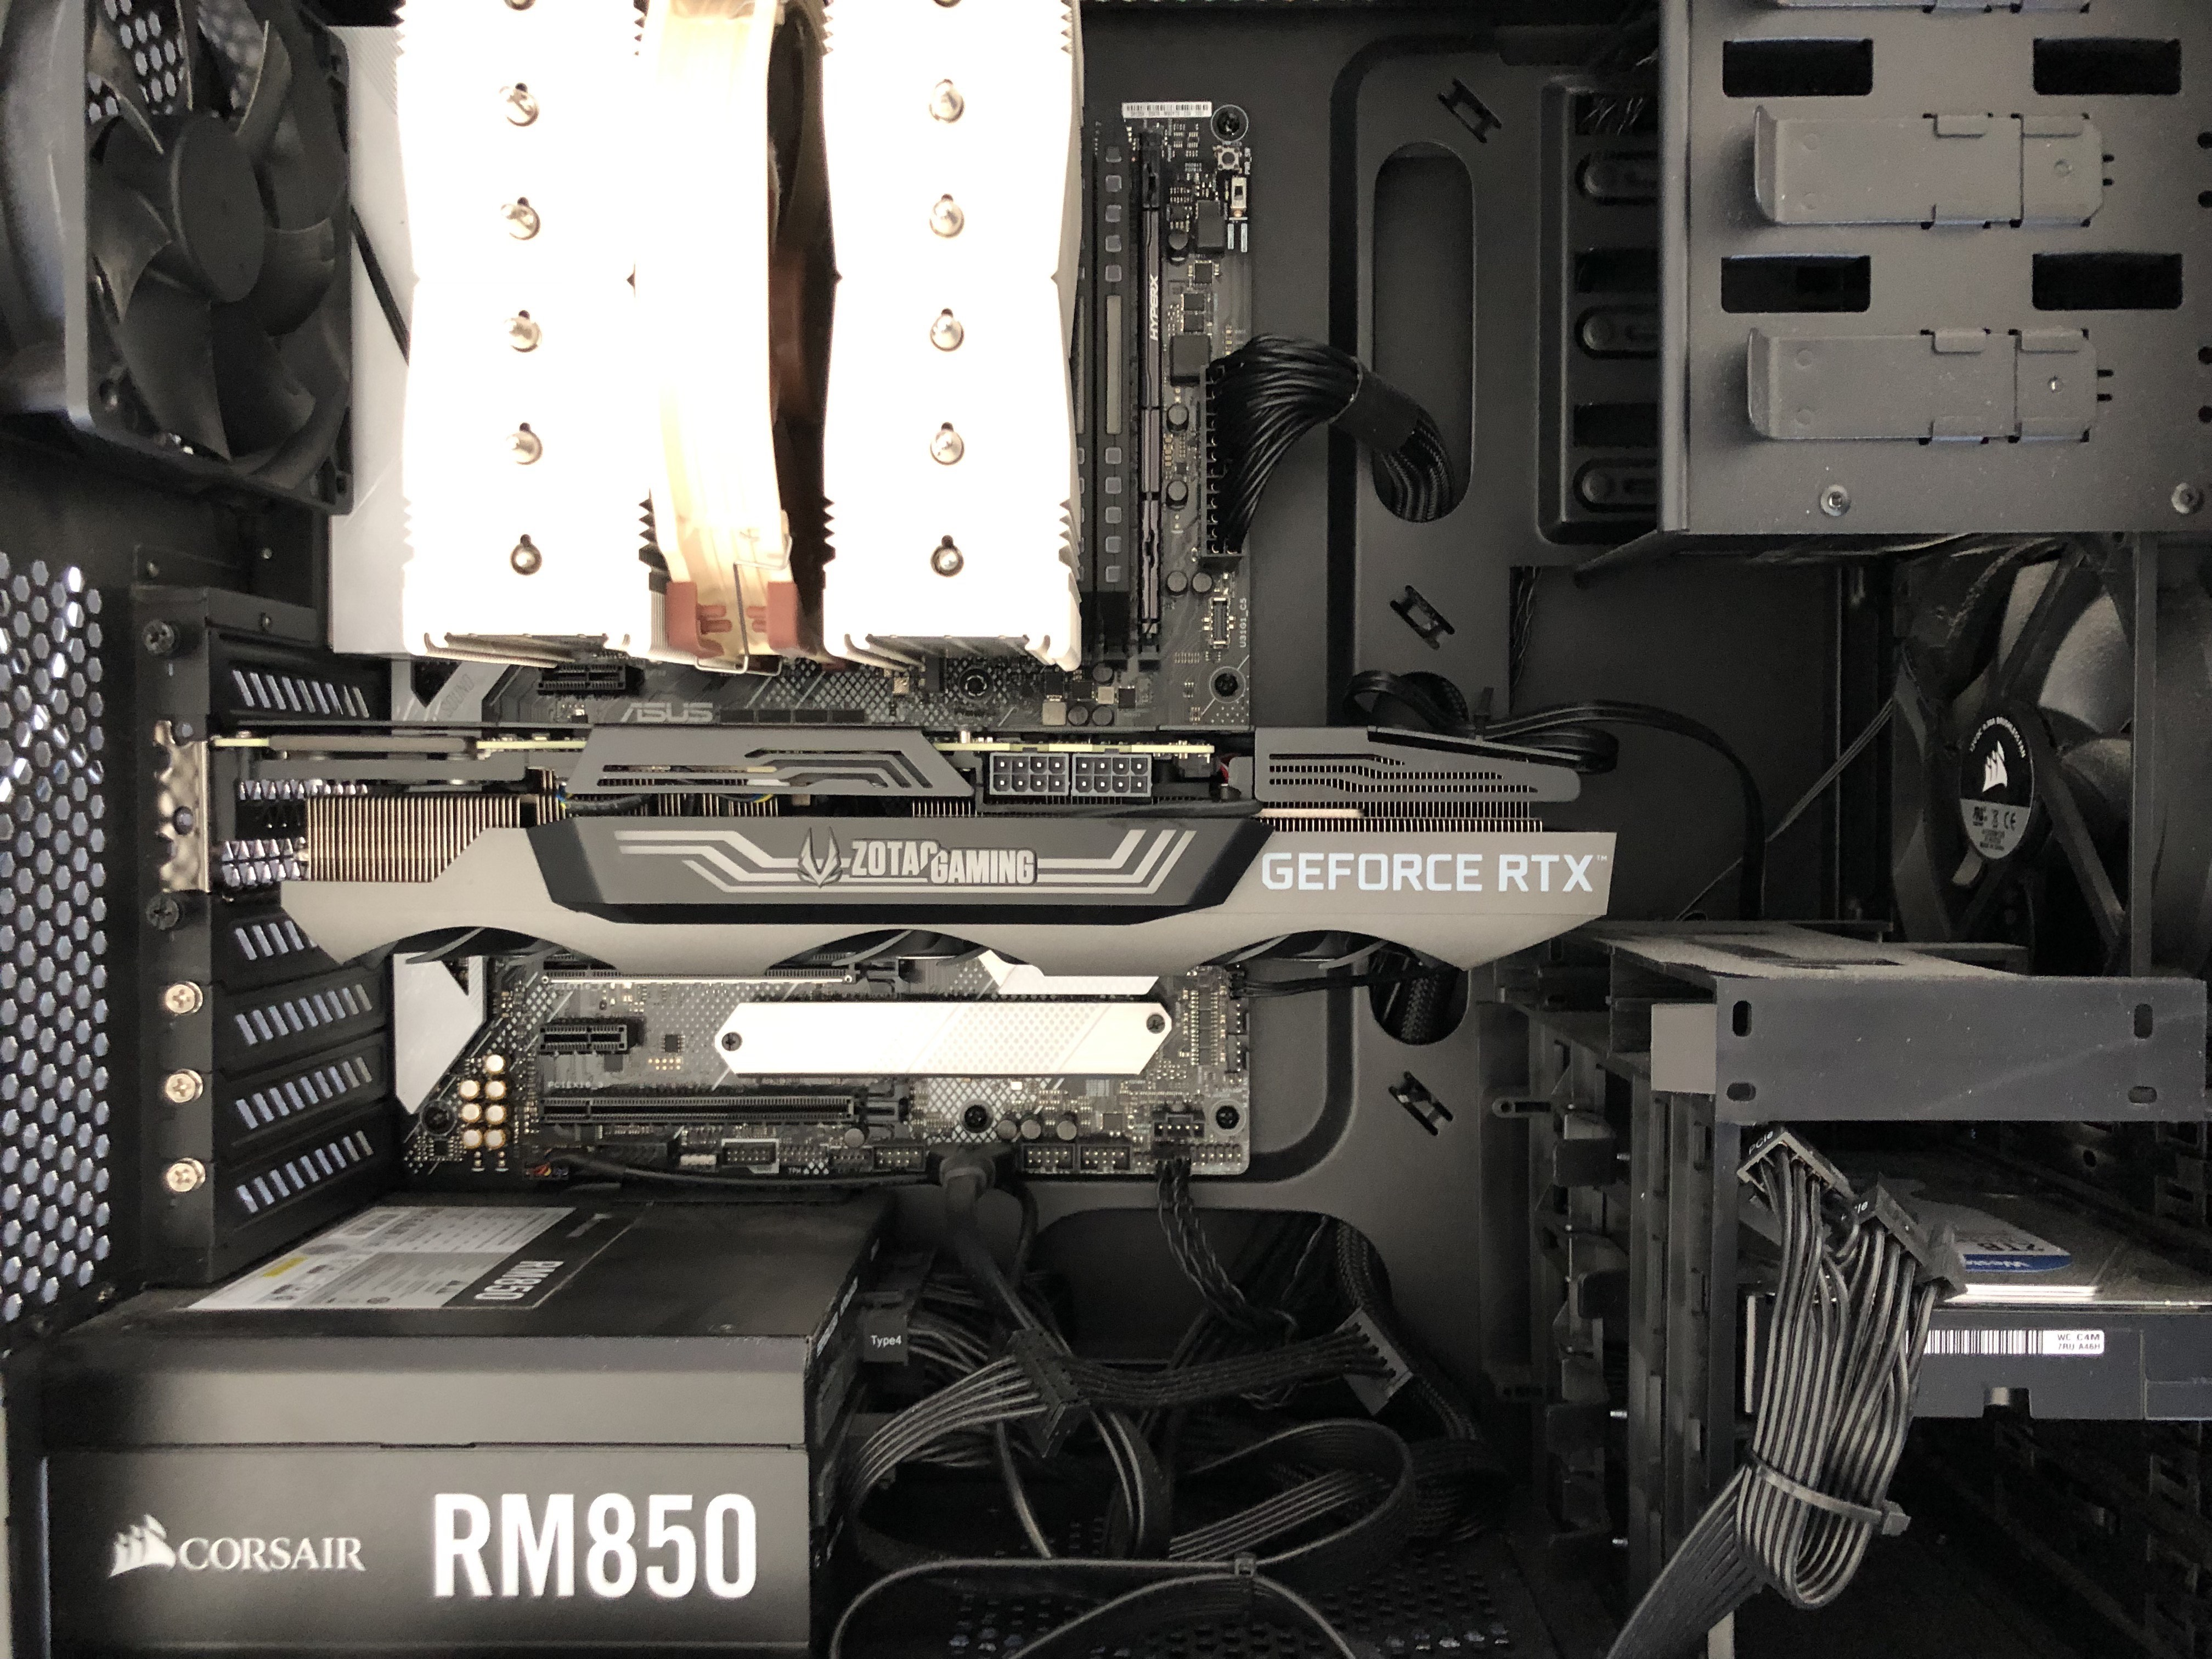
\includegraphics[width=.9\linewidth]{./figures/gpu_1.jpeg}
\end{figure}
\end{minipage}
\begin{minipage}{0.45\linewidth}
\begin{figure}
                        \centering
                        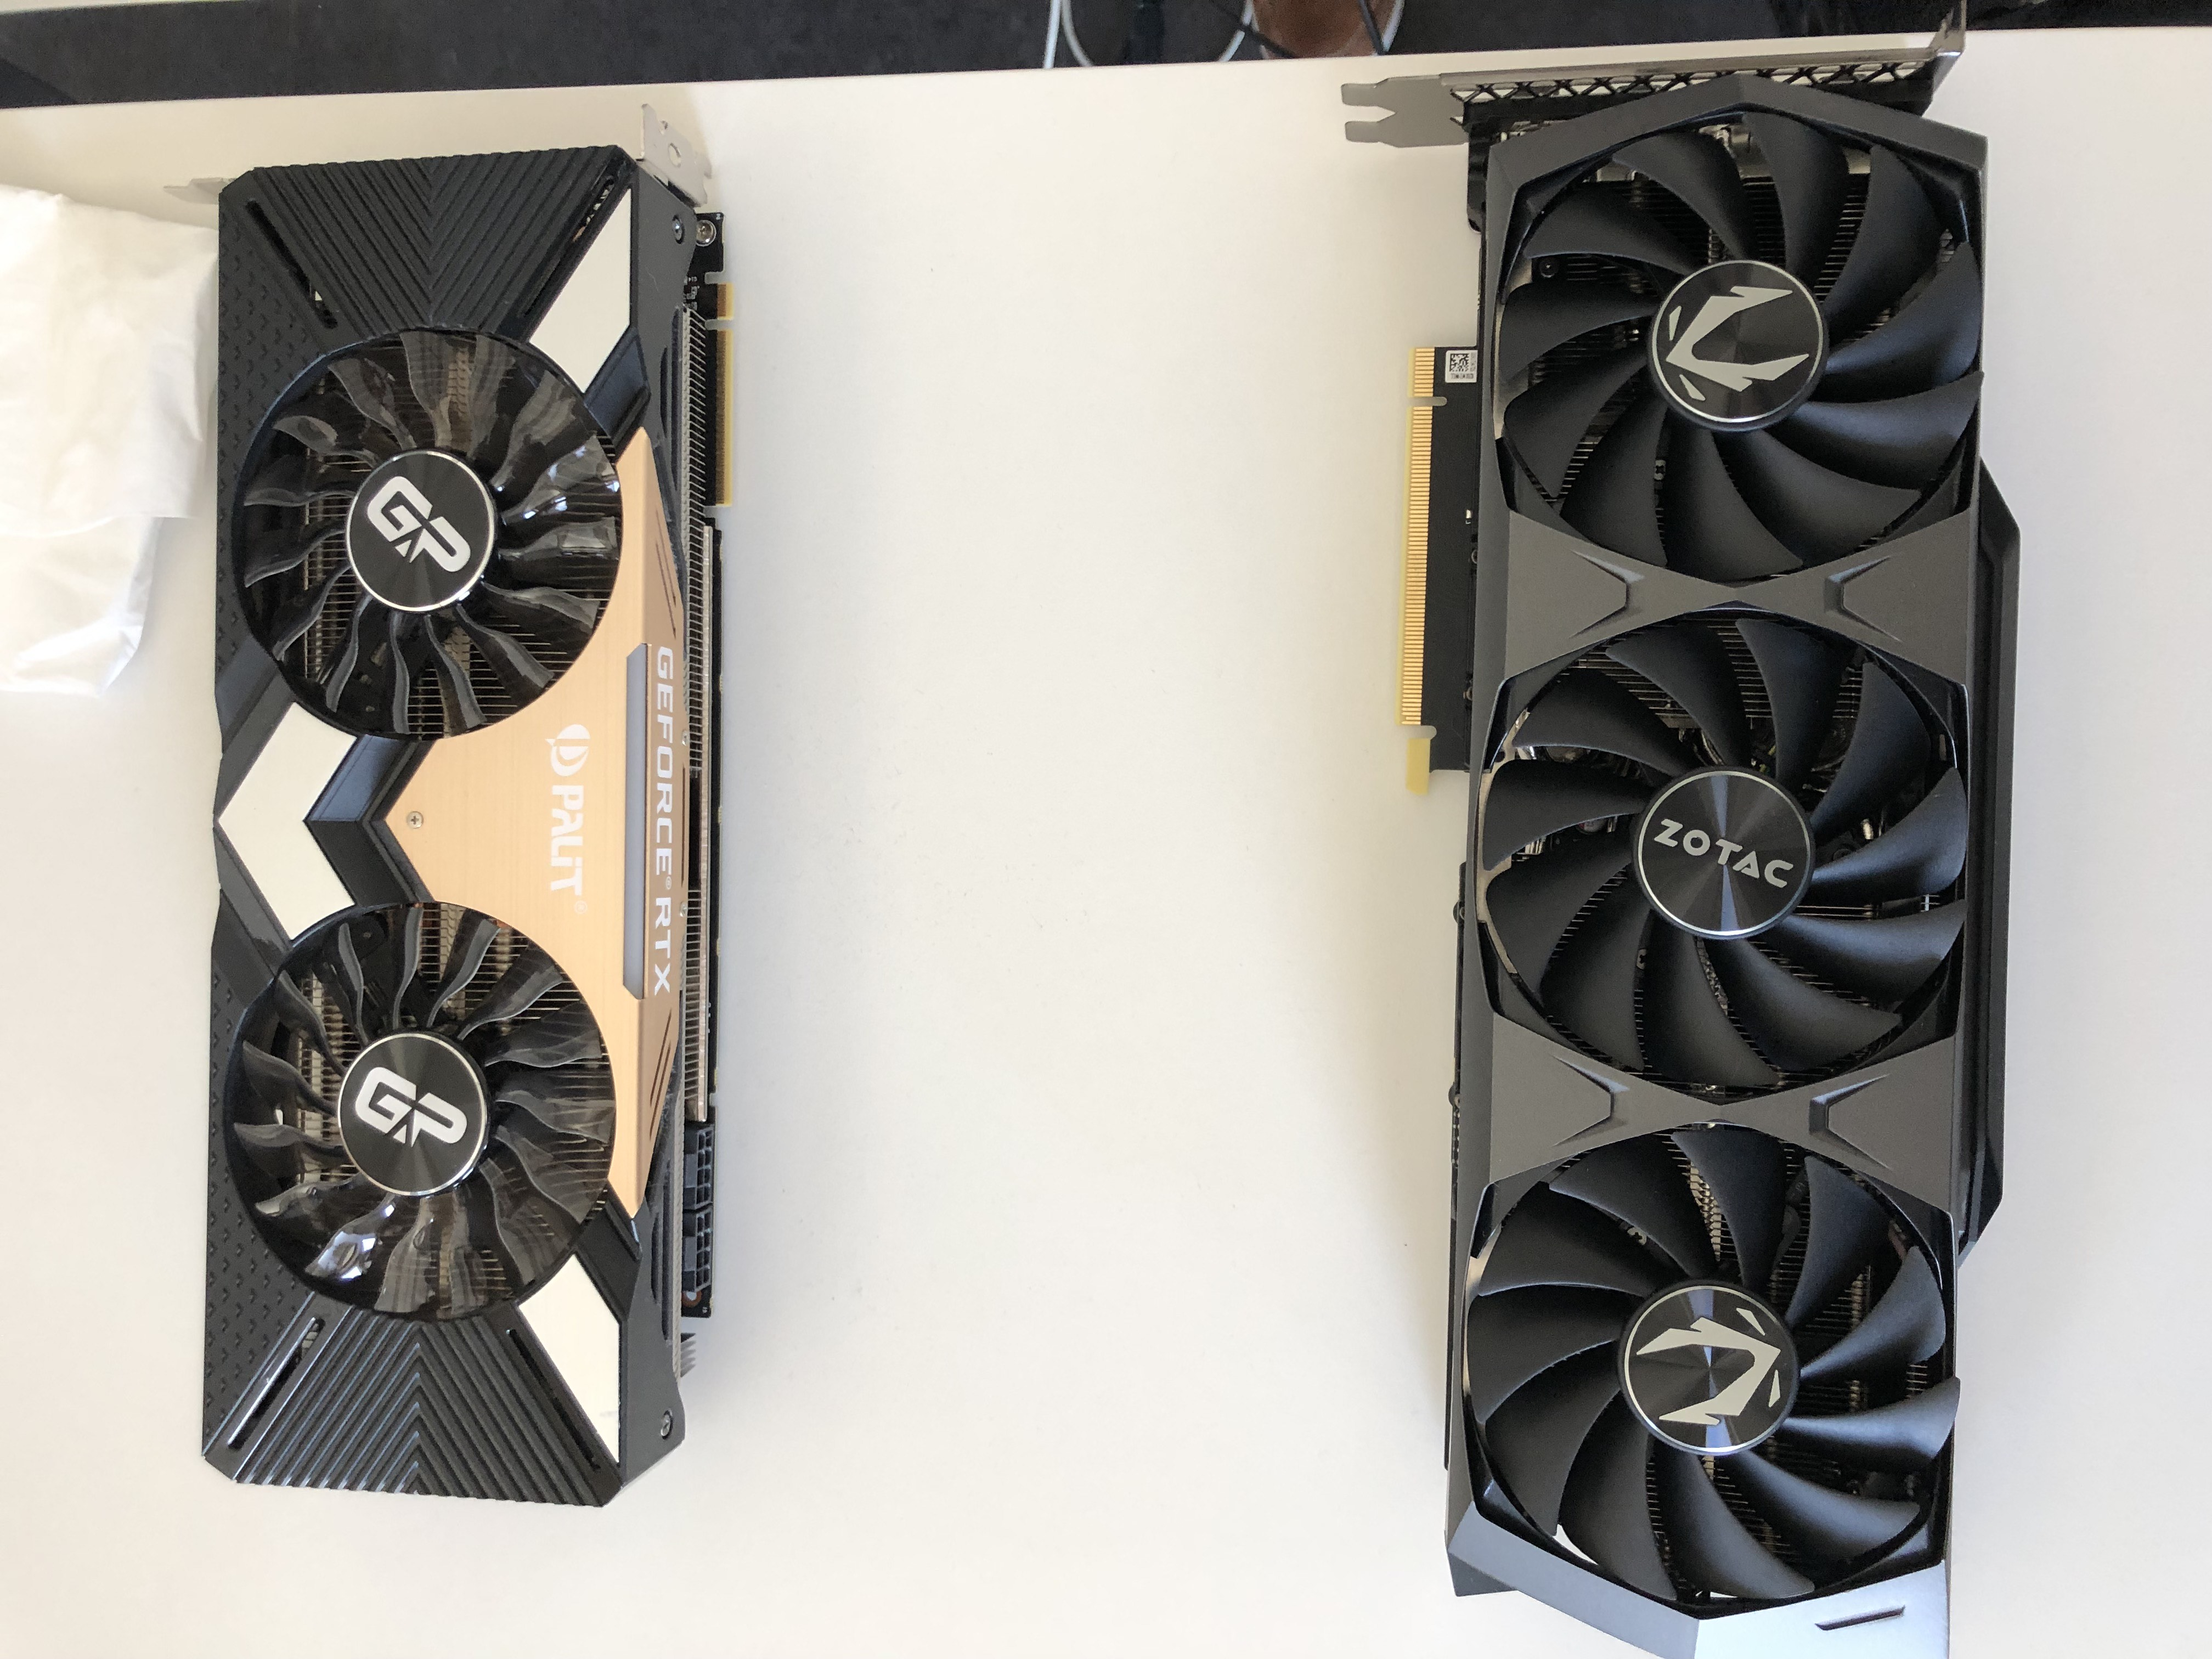
\includegraphics[width=.9\linewidth]{./figures/gpu_2.jpeg}
\end{figure}
\end{minipage}
\end{frame}

\begin{frame}[fragile]{Tensors on GPU? (cont'd)}
\vspace{-3mm}
Again: GPU is a hardware!\\
\begin{itemize}
\item To compute using GPU, you need to copy tensors to GPU memory.
\item Every \code{torch.Tensor} has the \code{device} attribute (basically CPU or GPU, tells the device on which the tensor is stored.).
\item Straightforward to transfer between devices in PyTorch \codeb{x.to(device)}:
\end{itemize}
\begin{python}
>>> device = torch.device(
...     "cuda:0" if torch.cuda.is_available() else "cpu")
>>> a = torch.rand([2, 3])
>>> a.device
device(type='cpu')
>>> b = a.to(device)  # copy to GPU.
>>> b.device
device(type='cuda', index=0)
\end{python}
\begin{itemize}
\item You can also directly create a tensor on a specific device \codeb{a = torch.rand([2, 3], device='cuda')}
\end{itemize}

NB: \codeb{to} is a method introduced after version $\geq$ 0.4.\\ (Used to be \code{x.cuda()} and \code{x.cpu()} before)
\end{frame}

\begin{frame}[fragile]{A few words on GPUs}
\vspace{-3mm}
\begin{itemize}
\item Different GPUs have different specs. Better GPUs released every year.
\item For example, on the USI's ICS cluster:
\begin{itemize}
\item NVIDIA GeForce GTX \textbf{1080} \textbf{8\,GB}
\item NVIDIA GeForce GTX \textbf{1080 Ti 11\,GB}
\item NVIDIA GeForce GTX \textbf{2080 Ti 11\,GB} (faster than 1080).
\end{itemize}
\item Be aware of the GPU memory of the machine.\\
Classic error you will get:\\
\codeb{RuntimeError: CUDA out of memory. Tried to allocate ...}
\item A typical solution is to reduce the batch size...
\item or run on machines which has more GPU memory.
\end{itemize}

\end{frame}

%\begin{frame}{Reminder: backpropagation}
%equations? illustrate it's painful to do it by hands?
%\end{frame}

\begin{frame}{Automatic differentiation}
Reminder: for gradient descent
$\theta(n+1) = \theta(n) - \alpha * \nabla_{\theta} \mathcal{L}(\theta(n))$\\
you need to compute the \textbf{gradient} of the loss $\nabla_{\theta} \mathcal{L}(\theta(n))$ w.r.t. the model parameters. Need to do backpropagation!\\
\vsp
\vsp
In PyTorch, this computation is \textbf{automatic}:
\begin{itemize}
\item Write computations of a scalar \codeb{loss} as a function of some tensors.
\item \codeb{loss.backward()} computes \textit{all} gradients\\ i.e. \textbf{no need to write these computations by yourself}.
\item \textit{all}? Every \codeb{torch.Tensor} has \codeb{requires\_grad} attribute.
\end{itemize}
\vsp
If interested in learning how this works; see e.g. \link{https://www.youtube.com/watch?v=MswxJw-8PvE}
\end{frame}

\begin{frame}[fragile]{Automatic differentiation (cont'd)}
Illustration:
\begin{python}
>>> import torch
>>> x = torch.tensor(2, requires_grad=True, dtype=torch.float32)
>>> x
tensor(2., requires_grad=True)
>>> y = torch.tensor(3, requires_grad=True, dtype=torch.float32)
>>> z = x * x + y  # Forward computation.
>>> z.backward()  # "dz/dx = 2 x"
>>> x.grad
tensor(4.)
\end{python}
\end{frame}

\begin{frame}[fragile]{Automatic differentiation (cont'd)}
\vspace{-3mm}
Note: gradients are accumulated.\\
Continue from the previous slide:
\begin{python}
>>> a = x * x + y  # define one more tensor.
>>> a.backward()  # add "da/dx" to "x.grad"
>>> x.grad  # contains "dz/dx + da/dx"
tensor(8.)
\end{python}
If this is not wanted, you need to reset it:
\begin{python}
>>> x.grad.data.zero_()  # reset gradient for x.
tensor(0.)
>>> a = x * x + y
>>> a.backward()
>>> x.grad
tensor(4.)
\end{python}
\textbf{In practice, you will not even need to do this for each parameter,
as you will be using some optimizer.} Examples later.
\end{frame}

\begin{frame}[fragile]{\textit{Detach} a tensor from gradient computation}
\vspace{-3mm}
You can use \texttt{detach()} to extract the value of a tensor such that its usage will
not influence the gradient computation.
\begin{python}
>>> x = torch.tensor([2., 3.], requires_grad=True)
tensor([2., 3.], requires_grad=True)
>>> y = x.detach()
tensor([2., 3.])
\end{python}
\end{frame}


%\begin{frame}{Computational graph}
%Excursion.\\
%define-by-run etc.
%\end{frame}

\begin{frame}{Example problem solving}
\vspace{-3mm}
\textbf{Regression task}:
\vsp
\begin{itemize}
\item Let $D$ be a positive integer. We have $N$ i.i.d. data points $\{(x_1, y_1), ..., (x_N, y_N)\}$ where $x_i\in \mathbb{R}^D$, $y_i\in \mathbb{R}$ for all $1 \leq i \leq N$.\\
\item We want to find a function $f_{\theta}$ parameterized by $\theta$ (a set of real numbers), which predicts $y$ from unseen $x$.
\item \textbf{Linear regression}: use $f_{\theta}(x) = w^\intercal x + b$\\
where $w \in \mathbb{R}^D$ and $b \in \mathbb{R}$ are \emphbf{model parameters}. So $\theta = \{w, b\}$.
\end{itemize}
\vsp \vsp
\textbf{Illustration for $D=1$}.\\
\vsp
\hspace{5mm}
\begin{minipage}{0.4\linewidth}
\begin{figure}
                        \centering
                        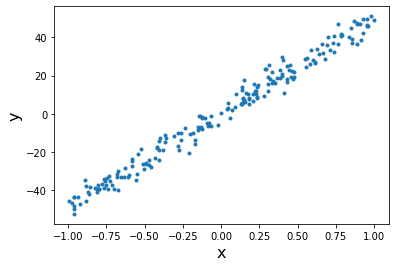
\includegraphics[width=.9\linewidth]{./figures/regression.png}
\end{figure}
\end{minipage}
\begin{minipage}{0.4\linewidth}
\begin{figure}
                        \centering
                        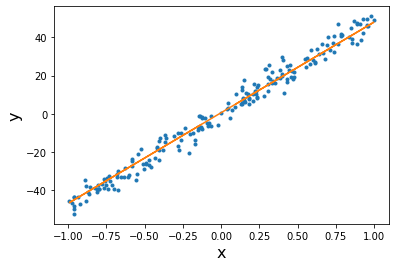
\includegraphics[width=.9\linewidth]{./figures/regression_example.png}
\end{figure}
\end{minipage}

\textbf{$D=1$ in all what follows}.
\end{frame}


\begin{frame}{Linear regression (with $D=1$)}
\vspace{-5mm}
\begin{itemize}
\item We have $N$ i.i.d. data points $\{(x_1, y_1), ..., (x_N, y_N)\}$ where $x_i\in \mathbb{R}$ $y_i\in \mathbb{R}$ for all $1 \leq i \leq N$.\\
\item Our linear model $f_{w, b}(x) = w * x + b$ has two parameters: $w \in \mathbb{R}$ and $b \in \mathbb{R}$.
\item We estimate these \emphbf{parameters} by minimizing \emphbf{mean squared error (MSE)} between model predictions and the actual data through \emphbf{gradient descent}.
\end{itemize}
\vsp
\pause
\textbf{Algorithm:}
\begin{itemize}
\item Randomly initialize the model parameters: $w_0 \in \mathbb{R}$ and $b_0 \in \mathbb{R}$.
\item Choose \emphbf{hyper-parameters}: learning rate $\alpha$ \& number of training steps $T$.
\item Repeat the following training steps $T$ times. At each step $t$ (from 0 to $T-1$):
\vspace{-3mm}
\begin{itemize}
\item Compute the MSE loss using the current value of $w_t$ and $b_t$: $\displaystyle \mathcal{L}(w_t, b_t) = \dfrac{1}{N} \sum_{i=1}^N \|f_{w_t, b_t}(x_i) - y_i  \|^2$
\item Compute the corresponding gradients: $\dfrac{\partial \mathcal{L}}{\partial w}(w_t, b_t)$ and $\dfrac{\partial \mathcal{L}}{\partial b}(w_t, b_t)$
\item Update parameters: $w_{t+1} = w_{t} - \alpha \dfrac{\partial \mathcal{L}}{\partial w}(w_t, b_t)$ and   $b_{t+1} = b_{t} - \alpha \dfrac{\partial \mathcal{L}}{\partial b}(w_t, b_t)$
\end{itemize}
\end{itemize}
Code? PyTorch?
\end{frame}


\begin{frame}[fragile]{Linear regression\\ How to generate data points?}

This is a ``toy task.'' We synthetically generate $N$ data points:
\begin{itemize}
\item For that, we start by setting the "true" $w^*$ and $b^*$ (that we choose).
\item We randomly sample $x_i$. Using that we compute $\hat{y}_i = w * x_i + b$.
\item Add a Gaussian noise: $y_i = \hat{y}_i + \epsilon_i$ with $\epsilon_i \sim \mathcal{N}(0, \sigma^2)$
where $\sigma$ is the standard deviation (that we choose).
\item We end up with noisy data points: $(x_i, y_i)$
\end{itemize}
\begin{python}
import numpy as np

def create_dataset(sample_size=10, sigma=0.1, w_star=1, b_star=1,
                   x_range=(-1, 1), seed=0):
    """Create data points for linear regression."""
    random_state = np.random.RandomState(seed)
    x_min, x_max = x_range
    x = random_state.uniform(x_min, x_max, (sample_size))
    y = x * w_star + b_star
    y += random_state.normal(0.0, sigma, (sample_size))

    return x, y

\end{python}
\end{frame}

\begin{frame}[fragile]{Linear regression (cont'd)\\ How to generate data points?}
% \vspace{-6mm}
\begin{itemize}
\item Generate the training data:
\end{itemize}
\begin{python}
num_samples = 200
sigma = 4
w_star = 50
X, y = create_dataset(
    sample_size=num_samples, sigma=sigma, w_star=w_star, seed=0)
\end{python}
\vsp
\begin{itemize}
\item From the same distribution, also sample the \emphbf{validation} data points using a different \emphbf{seed}:
\end{itemize}
\begin{python}
val_num_samples = 200
X_val, y_val = create_dataset(
    sample_size=num_samples, sigma=sigma, w_star=w_star, seed=42)
\end{python}
\end{frame}

\begin{frame}[fragile]{Linear regression (cont'd)\\ How to generate data points?}
% \vspace{-6mm}
\begin{itemize}
\item Visualize the data:
\end{itemize}
\begin{python}
import matplotlib.pyplot as plt

fig, ax = plt.subplots()
ax.set_xlabel("x", fontsize=16)
ax.set_ylabel("y", fontsize=16)

ax.plot(X, y, ".")
\end{python}
\begin{figure}
                        \centering
                        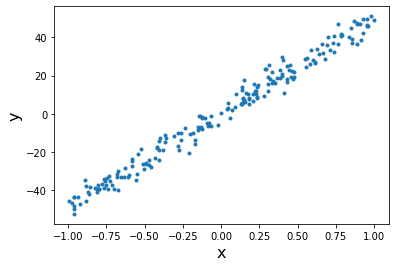
\includegraphics[width=.45\linewidth]{./figures/regression.png}
\end{figure}
\vspace{-5mm}
Check the documentation!
\end{frame}

\begin{frame}[fragile]{Linear regression, basic components}
\vspace{-6mm}
All necessary components are already implemented in PyTorch.
\begin{itemize}
\item We need a linear model $f$: $f_{\theta}(x) = w * x + b$\\
where $w \in \mathbb{R}$ and $b \in \mathbb{R}$ are the model parameters.
Build-in model in PyTorch is \codeb{torch.nn.Linear}.
\item We need the mean squared error:
\codeb{torch.nn.MSELoss}.
\item We update the model parameters using gradient descent.
The corresponding optimizer class is \codeb{torch.optim.SGD}
\end{itemize}
\begin{python}
import torch
import torch.nn as nn
import torch.optim as optim

DEVICE = torch.device("cuda:0" if torch.cuda.is_available()
                      else "cpu")

model = nn.Linear(1, 1)  # input dimension 1, and output dimension 1.
model = model.to(DEVICE)
loss_fn = nn.MSELoss()
learning_rate = 0.1
optimizer = optim.SGD(model.parameters(), lr=learning_rate)
\end{python}
\end{frame}

\begin{frame}[fragile]{Linear regression (cont'd)}
\vspace{-6mm}
Illustration of components (try on your own!):
\begin{itemize}
\item \codeb{torch.nn.Linear}.
\end{itemize}
\begin{python}
>>> import torch
>>> model = torch.nn.Linear(1, 1)
>>> model.weight
Parameter containing:
tensor([[-0.6464]], requires_grad=True)
>>> model.bias
Parameter containing:
tensor([-0.7324], requires_grad=True)
>>> x = torch.tensor([3.])
>>> model(x)
  # -0.6464 * 3. - 0.7324
tensor([-2.6717], grad_fn=<AddBackward0>)
\end{python}
\begin{itemize}
\item Recommendation: read documentation of \codeb{torch.nn.Linear}.
\item[-] e.g., how are the parameters initialized by default? 
\end{itemize}

\end{frame}

\begin{frame}[fragile]{Linear regression (cont'd)}
\vspace{-6mm}
\begin{itemize}
\item \codeb{torch.nn.MSELoss}.
\end{itemize}
\begin{python}
>>> import torch
>>> loss = torch.nn.MSELoss()
>>> a = torch.tensor([2.])
>>> b = torch.tensor([2.2])
>>> loss(a, b)
tensor(0.0400)
\end{python}
\begin{itemize}
\item \codeb{torch.optim.SGD}
\end{itemize}
\begin{python}
>>> import torch
>>> x = torch.tensor(2., requires_grad=True)
>>> z = x * x
>>> opt = torch.optim.SGD([x], lr=0.1)
>>> z.backward()
>>> opt.step()
>>> x
tensor(1.6000, requires_grad=True)
\end{python}
Again: \textbf{try on your own!} read documentation.
\end{frame}

\begin{frame}[fragile]{Linear regression (cont'd)}
\vspace{-6mm}
\begin{itemize}
\item Back to our regression problem.
\item The rest is to run the training loop.
\item But before that, data shape/dtype/device must be prepared as expected
by the function which will take them as input.
\end{itemize}

\begin{python}
X = X.reshape(num_samples, 1)  # shape expected by nn.Linear
X = torch.from_numpy(X)  # convert to torch.tensor
X = X.float()  # convert to float32 (from numpy double).
X = X.to(DEVICE)  # copy data to GPU.

# Same for other variables:
y = torch.from_numpy(y.reshape((num_samples, 1))).float().to(DEVICE)
X_val = torch.from_numpy(
  X_val.reshape((val_num_samples, 1))).float().to(DEVICE)
y_val = torch.from_numpy(
  y_val.reshape((val_num_samples, 1))).float().to(DEVICE)

\end{python}
\end{frame}

\begin{frame}[fragile]{Linear regression (cont'd)}
\vspace{-6mm}
Run the training loop.
\begin{python}
num_steps = 50  # We do 50 steps of gradient updates.

for step in range(num_steps):
    model.train()  # systematic: put model in 'training' mode.
    optimizer.zero_grad()  # systematic: start step w/ zero gradient.

    y_ = model(X)  # do prediction using the current model.
    loss = loss_fn(y_, y)  # compute error.
    print(f"Step {step}: train loss: {loss}")  # print train loss

    loss.backward()  # compute gradients.
    optimizer.step()  # update parameters

    # Eval on validation set
    model.eval()  # systematic: put model in 'eval' mode.
    # everything below does not contribute to gradient computation
    with torch.no_grad():
        y_ = model(X_val)
        val_loss = loss_fn(y_, y_val)
    print(f"Step {step}: val loss: {val_loss}") 

\end{python}
Or: \codeb{model.zero\_grad()} instead of \codeb{optimizer.zero\_grad()}.
\end{frame}

\begin{frame}[fragile]{Linear regression (cont'd)}
\vspace{-6mm}
Plot the resulting model:
\begin{python}
# Get the prediction from the final model.
model.eval()
with torch.no_grad():
    y_ = model(X)
fig, ax = plt.subplots()
ax.plot(X.cpu().numpy(), y.cpu().numpy(), ".")
ax.plot(X.cpu().numpy(), y_.cpu().numpy(), "-")

ax.set_xlabel("x", fontsize=16)
ax.set_ylabel("y", fontsize=16)
\end{python}
\begin{figure}
                        \centering
                        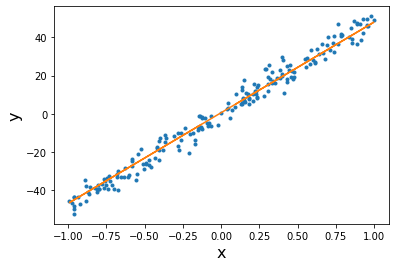
\includegraphics[width=.5\linewidth]{./figures/regression_example.png}
\end{figure}
\end{frame}


\begin{frame}[fragile]{Linear regression (cont'd)}
\vspace{-6mm}
We can also take a look at the final model parameters:
\begin{python}
>> model.weight
Parameter containing:
tensor([[47.3805]], device='cuda:0', requires_grad=True)
>> model.bias
Parameter containing:
tensor([0.5539], device='cuda:0', requires_grad=True)
\end{python}
\begin{itemize}
\item This was a simple example problem to illustrate some PyTorch functionalities.
\item A similar problem is to be solved in the \emphbf{Assignment 1}.
\item In the next lectures, we look into more details of components for building systems.
\end{itemize}
\end{frame}


\begin{frame}{A few words on \emphbf{Exercise 2 \& 3}}
\textbf{Now: Exercise 2}
\begin{itemize}
\item Objective: get familiar with PyTorch basics.
\end{itemize}
\vsp
\vsp
\emphbf{Next week: Assignment 1 (Exercise 3)}
\begin{itemize}
\item First assignment
\item Contributes to 15\% of the final grade.
\item Task: polynomial regression
\item You will be using many basic tools that you have learned:
\begin{itemize}
\item numpy random number generator
\item plot data points
\item ...
\end{itemize}
\end{itemize}
\end{frame}
% -----------------------------------------------------------------------
\subsection{Implementation of Systems}
\begin{frame}{Implementation of Systems}
\textbf{What do we need?} Reminder:
\vsp
\begin{itemize}
\item Dataset
\item Model
\item Loss
\item Optimizer
\item Multiple optimization steps (training loop).
\end{itemize}
\end{frame}

\begin{frame}[fragile]{Structure Preview: Sketch}
\vspace{-6mm}
\begin{python}
device = torch.device('cuda')  # 'cuda' for GPU.
dataset = MyDataset(...)
dataloader = DataLoader(dataset, ...) 

model = MyModel(...)
model = model.to(device)  # put the model params on device.
optimizer = torch.optim.SGD(model.parameters(), lr = 0.01)
loss_fn = Loss(...)

for i in range(10):  # Training loop for 10 epochs.
    for sample in dataloader:  # get batch.
        data = sample['data'].to(device)
        target = sample['target'].to(device)

        prediction = model(data)
        loss = loss_fn(prediction, target)

        optimizer.zero_grad() # reset the gradients
        loss.backward()
        optimizer.step()  # update params.
    # validation.
        # compute validation loss ...
        # save the intermediate model, ...
\end{python}
% training_loss += loss.item()
\end{frame}

\begin{frame}{Implementing datasets / dataloader}
For SGD, we need to generate data batches (i.e. randomly sampled training examples).\\
\vsp
\textbf{Two useful classes} in \code{torch.utils.data}
\begin{itemize}
\item \codeb{torch.utils.data.Dataset}: class for representing the dataset.
\item \codeb{torch.utils.data.Dataloader}: class for generating batches of data (does e.g. shuffling).
\end{itemize}
\vsp
Official tutorial: \link{https://pytorch.org/tutorials/beginner/data_loading_tutorial.html}
\end{frame}

\begin{frame}[fragile]{Dataset}
\vspace{-4mm}
\textbf{Three main methods:}
\begin{itemize}
\item \code{\_\_init\_\_(self)}
\item \code{\_\_getitem\_\_(self, index)}
\item \code{\_\_len\_\_(self)}
\end{itemize} 
\begin{python}
from torch.utils.data import Dataset, DataLoader

class RandomDataset(Dataset):

    def __init__(self, data_dim, num_data_points):
        self.len = num_data_points
        self.data = torch.randn(num_data_points, data_dim)

    def __getitem__(self, index):
        return self.data[index]

    def __len__(self):
        return self.len
\end{python}
\end{frame}

\begin{frame}[fragile]{Dataloader}
Generate batches.\\
Continue from the previous slides:
\begin{python}
input_dim = 10 
data_size = 1000
rand_dataset = RandomDataset(input_dim, data_size)

batch_size = 32
data_loader =
  DataLoader(dataset=rand_dataset,
             batch_size=batch_size, shuffle=True)

for i, data in enumerate(data_loader, 0):
    # each data contains 32 random samples of the data
    # data can then be to be fed to the model.
    ...
\end{python}
One can also specify a more specific way of sampling batches e.g. via \codeb{sampler} argument of \codeb{DataLoader}.
Alternatively: you could also implement your own data loader.
\end{frame}

\begin{frame}{Implementing models using PyTorch}
PyTorch \textbf{models} are regular Python class which inherits from \codeb{torch.nn.Module}\\
\vsp
\textbf{Two main methods}
\begin{itemize}
\item \codeb{\_\_init\_\_(self)}: define model components.
\item \codeb{forward(self, x)}: forward computation, given input $x$.
\end{itemize}
\end{frame}

\begin{frame}[fragile]{PyTorch Models, example}
\vspace{-8mm}
\begin{python}
import torch.nn as nn
import torch.nn.functional as F

class MyModel(nn.Module):

    def __init__(self, input_size, output_size):
        super(MyModel, self).__init__()
        self.fc = nn.Linear(input_size, output_size)

    def forward(self, input):
        output = self.fc(input)
        output = F.relu(output)
        return output
\end{python}
Note: model itself can contain \codeb{nn.Module} object, here \codeb{nn.Linear} a linear transformation layer.\\
These basic building blocks are already implemented; ready to be used.
\end{frame}

%\begin{frame}[fragile]{Put together, training example}
%\vspace{-8mm}
%\begin{python}
%import torch.nn as nn
%import torch.nn.functional as F
%
%class Net(nn.Module):
%    def __init__(self):
%        super(Net, self).__init__()
%        self.conv1 = nn.Conv2d(3, 6, 5)
%        self.pool = nn.MaxPool2d(2, 2)
%        self.conv2 = nn.Conv2d(6, 16, 5)
%        self.fc1 = nn.Linear(16 * 5 * 5, 120)
%        self.fc2 = nn.Linear(120, 84)
%        self.fc3 = nn.Linear(84, 10)
%\end{python}
%\end{frame}

\begin{frame}[fragile]{Checking model information}
\pause
\vspace{-6mm}
Continue from last slide.\\
\texttt{print} gives a decent overview:
% \begin{python}
%>>> model = MyModel(5, 2)
%>>> list(model.children())
%[Linear(in_features=5, out_features=2, bias=True)]
%\end{python}
\begin{python}
>>> model = MyModel(5, 2)
>>> print(model)
MyModel(
  (fc): Linear(in_features=2, out_features=5, bias=True)
)
\end{python}
\pause
Inspecting model parameters via \texttt{state\_dict()}:
\begin{python}
>>> for key, value in model.state_dict().items():
...    print(key)
...    print(value)
fc.weight
tensor([[ 0.1786,  0.4163, -0.0949,  0.0152,  0.4388],
        [-0.2598,  0.0871,  0.3840, -0.3750,  0.4289]])
fc.bias
tensor([0.0083, 0.1554])
\end{python}
%\pause
%\begin{python}
%>>> for module in model.named_modules():   # TODO check
%...   print(module)
%('', MyModel(
%  (fc): Linear(in_features=5, out_features=2, bias=True)
%))
%('fc', Linear(in_features=5, out_features=2, bias=True))
%\end{python}
\end{frame}

\begin{frame}[fragile]{Train vs. Evaluation Modes}
Some model components have different behaviors whether
it is in training or evaluation mode (e.g. dropout, batch normalization).
\pause
\vsp
\begin{itemize}
\item Run \codeb{model.train()} before training.
\item Run \codeb{model.eval()} before evaluation. 
\end{itemize}
\vsp
\pause
Also, to avoid modifying your model during evaluation,
you should everything under:
\begin{python}
with torch.no_grad():
    # evaluation
    ...
\end{python}
to prevent gradient computation (also saves memory).
\end{frame}

\begin{frame}[fragile]{Loss}
Different types of losses are available:
\begin{itemize}
\item \codeb{torch.nn.MSELoss}
\item \codeb{torch.nn.CrossEntropyLoss} (note: softmax is included in the loss computation)
\item etc...
\end{itemize}
\vsp
Illustration:
\begin{python}
>>> loss_fn = nn.MSELoss()
>>> predictions = torch.randn(3, 5, requires_grad=True)
>>> targets = torch.randn(3, 5)
>>> loss = loss_fn(predictions, targets)
>>> loss.backward()
\end{python}
\end{frame}

\begin{frame}[fragile]{Optimizer}
\vspace{-3mm}
Very much straightforward:
\begin{itemize}
\item Choose optimizer of your choice.\\
Most popular ones: \codeb{torch.optim.Adam} and \codeb{torch.optim.SGD}.
\item Do \codeb{optimizer.zero\_grad()} before backward computation.\\
Remember the gradients are accumulated.
\item Do \codeb{optimizer.step()}. It updates all params.
\end{itemize}
\begin{python}
optimizer = torch.optim.SGD(model.parameters(), lr = 0.01)

for sample in dataloader:
    data = sample['input'].to(device)
    target = sample['target'].to(device)
    prediction = model(data)
    loss = loss_fn(prediction, target)
    optimizer.zero_grad()  # reset gradients.
    loss.backward()
    optimizer.step()  # one step of update according to optimizer.
\end{python}
\end{frame}

\begin{frame}[fragile]{Saving \& Loading models}
\begin{itemize}
\item \codeb{torch.save}
\end{itemize}
\begin{python}
state = {'model_state' : model.state_dict(),
         'optimizer': optimizer.state_dict)}
torch.save(state, 'state.pt')
\end{python}
\vsp
\begin{itemize}
\item \codeb{torch.load}
\end{itemize}
\begin{python}
model = MyModel()
optimizer = optim.SGD(model_parameters(), lr=0.01)
checkpoint = torch.load('state.pt')
model.load_state_dict(checkpoint['model_state'])
optimizer.load_state_dict(checkpoint['optimizer_state'])
\end{python}
\vsp
Note: some optimizers also have some states which
must be stored, in order to resume training from
where it had been stopped. 
\end{frame}

\begin{frame}[fragile]{Monitoring training}
Finally, all pieces are essentially there!\\
\pause
\vsp
One last thing: \textbf{monitoring training process}.
\pause
\begin{itemize}
\item Training can take a long time. Depending on the task, it can take from a few days to a few months!\\ (fortunately not in our exercises.)
\pause
\item You would want to check the state of its progress by \textit{monitoring}
whether the training and validation losses are \textbf{going down}.
\pause
\item Also, you can detect very bad choices of (training) hyper-parameters, by checking the values of the training loss \textbf{just after a  few updates}!
\end{itemize}
$\rightarrow$ \emphbf{You will experience this in the exercises.}\\
\vsp
\vsp
\pause
Methods for monitoring:
\begin{itemize}
\item \textbf{Print the loss values} regularly, after each $n$ updates.
\item Use \textbf{visualization tools}: tensorboard, \textit{Weights \& Biases}, ...
\end{itemize}
\end{frame}

\begin{frame}[fragile]{Tensorboard}
\vspace{-5mm}
\begin{itemize}
\item Tool for visualizing and monitoring training.
\item Originally part of TensorFlow (Google).
\end{itemize}
\vsp
\pause
Basic idea:
\begin{itemize}
\item Add a few lines in your code to record the quantities of your interest in a log.
\item \texttt{tensorboard} provides visualization of the log (on a browser).
\end{itemize}
\pause
\begin{python}
from tensorboardX import SummaryWriter

writer = SummaryWriter(logdir='my-experiment/')

# ... inside the training loop ...
    # `train_steps` counts the training steps.
    # forward the model, compute loss etc
    writer.add_scalar('loss', loss, train_steps)
    # ...
    writer.add_scalar('train acc', train_acc, train_steps)
    # ... etc
\end{python}
(or \codeb{from torch.utils.tensorboard import SummaryWriter})
\end{frame}

\begin{frame}[fragile]{Tensorboard, illustration}
\begin{itemize}
\item You need to first install tensorboard: \codeb{pip install tensorboard}
\item Run \codeb{tensorboard --logdir my-experiment} on terminal.
\item This should give:\\ \texttt{TensorBoard 2.3.0 at http://localhost:6006/}
\item Paste it on your browser:
\end{itemize}
\begin{figure}
                        \centering
                        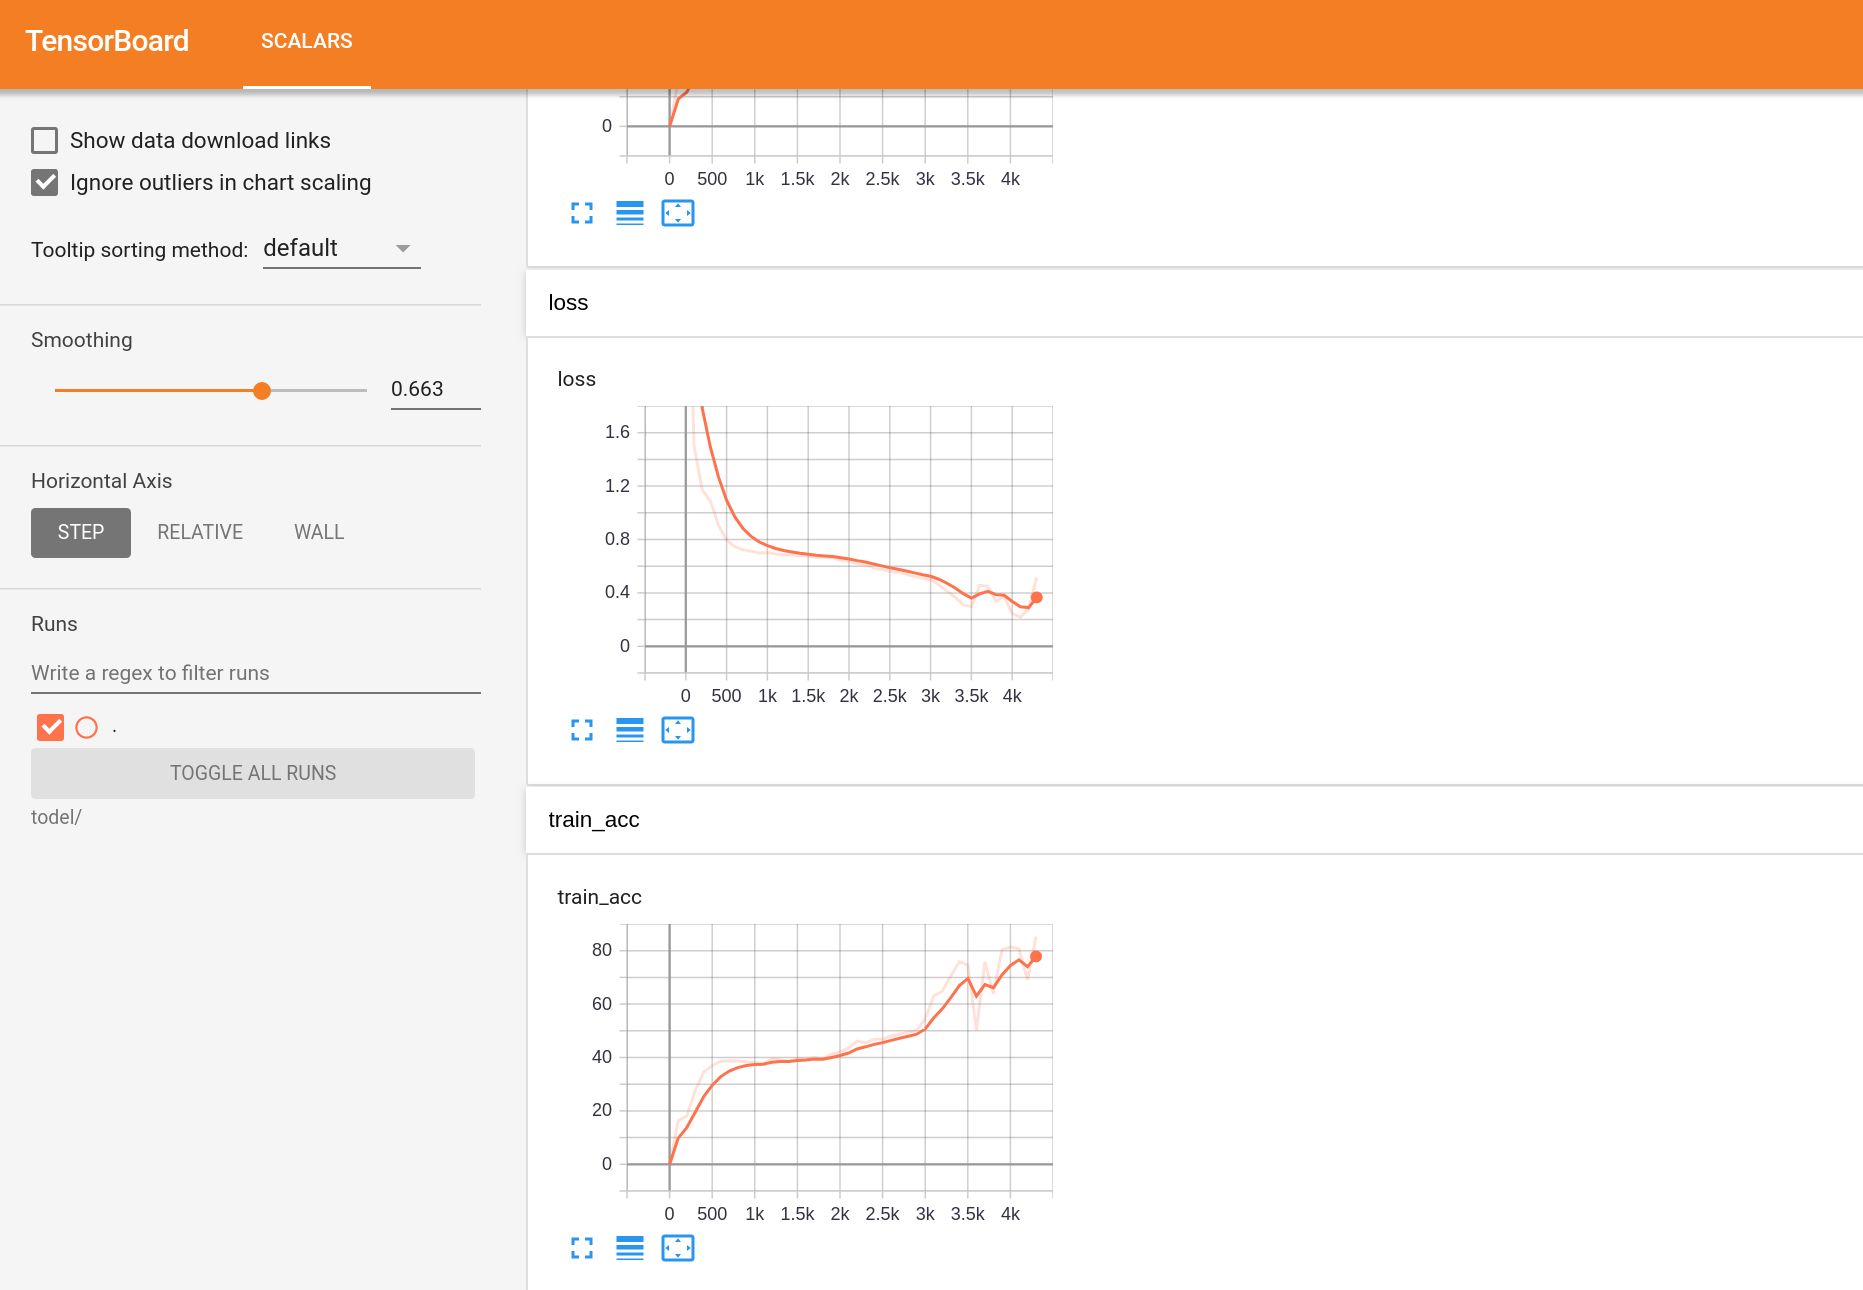
\includegraphics[width=.6\linewidth]{./figures/tensorboard.png}
% \vspace{-3mm}
\end{figure}
\end{frame}

%\begin{frame}{Put them all together!\\ example with linear regression}
%\TODO maybe directly MNIST with FF.
%\textbf{Regression task}:
%\begin{itemize}
%\item We have $N$ data points $\{(x_1, y_1), ..., (x_N, y_N)\}$ which are i.i.d.\\ $x_i\in \mathbb{R}^D$ $y_i\in \mathbb{R}$ for all $1 \leq i \leq N$.\\
%\item We want to find a function $f_{\theta}$ parametrized by $\theta$, which predicts well $y$ from $x$ for unseen $(x, y)$.
%\item Linear regression: use $f_{\theta}(x) = w . x + b$\\
%where $w \in \mathbb{R}^D$ and $b \in \mathbb{R}$ are model parameters. So $\theta = \{w, b\}$.
%\end{itemize}
%\end{frame}

\begin{frame}{Put them all together! Full example}
Let's consider \textbf{digit image classification} task using the MNIST dataset \citem{lecun1998mnist} and a two-layer \textbf{feed-forward neural network}:
\pause
\vsp
\begin{itemize}
\item Task: \textbf{classification} of images; each image is one handwritten digit (0 to 9).
\item[-] Input to the model: image.
\item[-] Output of the model: 10-dim vector, representing probability for each digit (10 classes).
\item[-] Can feed-forward models handle this problem? Yes.
\end{itemize}
\pause
\vsp
Basic statistics:
\begin{itemize}
\item 60\,K training images, 10\,K test images.
\item Dimension of each image: $\mathbb{R}^{28 \times 28}$, in black \& white (one channel),
\item[-] which can be reshaped to 784-dim vector, to input to the model.
\end{itemize}
\end{frame}

\begin{frame}[fragile]{Import packages... etc}
\vspace{-5mm}
\begin{python}
import torch
import torch.nn as nn
import torchvision
import torchvision.transforms as transforms
\end{python}

\begin{python}
device = torch.device(
    "cuda:0" if torch.cuda.is_available() else "cpu")
\end{python}

\begin{python}
# Hyper-parameters
# to specify model:
input_size = 784
hidden_size = 512
num_classes = 10

# for training:
num_epochs = 5
batch_size = 128
learning_rate = 0.001
momentum = 0.9
\end{python}
\end{frame}

\begin{frame}[fragile]{Create datasets/dataloader}
MNIST is standard dataset: you can directly get it from \code{torchvision}.
\begin{python}
# Datasets
train_set = torchvision.datasets.MNIST(
    root='./data', train=True, transform=transforms.ToTensor(), 
    download=True)

test_set = torchvision.datasets.MNIST(
    root='./data', train=False, transform=transforms.ToTensor())

# Dataloaders
train_loader = torch.utils.data.DataLoader(
    dataset=train_set, batch_size=batch_size, shuffle=True)

test_loader = torch.utils.data.DataLoader(
    dataset=test_set, batch_size=batch_size, shuffle=False)

\end{python}
\end{frame}

\begin{frame}[fragile]{Define model}
\begin{itemize}
\item We use a basic \textbf{feed-forward} neural network with 2 layers (one hidden vector) with the ReLU activation function.
\item[-] The dimension $d$ of the hidden vector is the \textbf{model hyper-parameter}.
\item[-] The input and output dimensions are specified by the problem.
\vsp
\pause
\item Input image $x \in \mathbb{R}^{784}$ (reshaped 28x28 image).
\item The first layer transforms $x \in \mathbb{R}^{784}$ to a hidden vector $h \in \mathbb{R}^{d}$:
\[
h = \ReLU(W_1x + b_1) = \max(W_1x + b_1, 0)
\]
$W_1 \in \mathbb{R}^{d \times 784}$ and $b_1 \in \mathbb{R}^{d}$ are \textbf{trainable/model parameters}.
\pause
\item The output layer transforms $h \in \mathbb{R}^{d}$ to a vector $y \in \mathbb{R}^{10}$
(size = number of classes = 10 digit):
\[
y = W_2h + b_2
\]
$W_2 \in \mathbb{R}^{10 \times d}$ and $b_2 \in \mathbb{R}^{10}$ are \textbf{trainable/model parameters}.
%\item $W_1 \in \mathbb{R}^{d \times 784}$, $W_2 \in \mathbb{R}^{10 \times d}$, $b_1 \in \mathbb{R}^{d}$, and $b_2 \in \mathbb{R}^{10}$
%are the trainable parameters of the model.
\pause
\item[-] Softmax function transforms the logit $y$ to a probability distribution: for $i \in \{0,..., 9\}$
\[
p(i|x) = \softmax(y)_i
\]
\end{itemize}
\end{frame}

\begin{frame}[fragile]{Define model, implementation}
\begin{python}
class FFModel(nn.Module):

    def __init__(self, input_size, hidden_size, num_classes):
        super(FFModel, self).__init__()
        self.fc1 = nn.Linear(input_size, hidden_size) 
        self.fc2 = nn.Linear(hidden_size, num_classes)  
    
    def forward(self, x):
        # Assume linealized input: here `images.view(-1, 28*28)`.
        out = self.fc1(x)
        out = F.relu(out)
        out = self.fc2(out)
        # second layer does not need activation function;
        # softmax is computed by cross entropy loss.
        return out
\end{python}
\end{frame}

\begin{frame}[fragile]{Create model, loss, optimizer}
\begin{python}
# Create model
model = FFModel(input_size, hidden_size, num_classes)
model = model.to(device)  # put all model params on GPU.

# Create loss and optimizer
loss_fn = nn.CrossEntropyLoss()

optimizer = optim.SGD(
    model.parameters(), lr=learning_rate, momentum=momentum)
\end{python}
\end{frame}

\begin{frame}[fragile]{Training}
\vspace{-5mm}
\begin{python}
# Training
for epoch in range(num_epochs):
    model.train()  # Set model in train mode.
    for i, (images, labels) in enumerate(train_loader):
        # shape of images is (B, 1, 28, 28).
        images = images.view(-1, 28*28)  # reshape to (B, 784).
        images = images.to(device)  # copy data to GPU.
        labels = labels.to(device)  # shape (B).

        outputs = model(images)  # shape (B, 10).
        loss = loss_fn(outputs, labels)

        optimizer.zero_grad()  # reset gradients.
        loss.backward()  # compute gradients.
        optimizer.step()  # update parameters.
        
        # here, print the current value of loss...
        # saving model checkpoint... to be done in Exercise!
\end{python}
\end{frame}

\begin{frame}[fragile]{Evaluation}
\vspace{-5mm}
\begin{python}
# Evaluation
with torch.no_grad():
    correct = 0
    total = 0
    model.eval()  # Set model in eval mode. Don't forget!
    for images, labels in test_loader:
        images = images.view(-1, 28*28)
        images = images.to(device)
        labels = labels.to(device)  # shape (B)
        outputs = model(images)  # shape (B, num_classes)
        # 'outputs' are logits (unnormalized log prob).
        # Model prediction is the class which has the highest
        # probability according to the model,
        # i.e. the class which has the highest logit value:
        _, predicted = outputs.max(dim=1)
        # predicted.shape: (B)
        total += labels.size(0)
        correct += (predicted == labels).sum().item()
    test_acc = 100 * correct / total

print(f'Test accuracy is: {test_acc} %')
\end{python}

%\begin{python}
%# Evaluation
%with torch.no_grad():
%    correct = 0
%    total = 0
%    model.eval()  # Set model in eval mode. Don't forget!
%    for images, labels in test_loader:
%        images = images.view(-1, 28*28)
%        images = images.to(device)
%        labels = labels.to(device)  # shape (B)
%        outputs = model(images)  # shape (B, num_classes)
%        # 'outputs' are logits (unnormalized log prob).
%        # Model prediction is the class which has the highest
%        # probability according to the model,
%        # i.e. the class which has the highest logit value:
%        _, predicted = torch.max(outputs.data, 1)
%        # predicted.shape: (B)
%        total += labels.size(0)
%        correct += (predicted == labels).sum().item()
%    test_acc = 100 * correct / total
%
%print(f'Test accuracy is: {test_acc} %')
%\end{python}
\end{frame}


\begin{frame}{Not covered in this example}
\begin{itemize}
\item Preparation of \emphbf{validation} dataset!\\ Crucial for tuning \emphbf{hyper-parameter}.
\item Hyper-parameter tuning.
\item Monitoring of intermediate model performance during training \& saving model parameters.
\item ... we will see more refinements to in the chapter after next one!
\end{itemize}
\vsp
You will do these in \emphbf{Exercise 4}!
\end{frame}

%\begin{frame}{Alternative frameworks}
%Libraries:
%TensorFlow, JAX, MXNet,
%High-level frameworks:
%keras,
%Even higher...
%fairseq etc...
%Why PyTorch?
%recent Popularity, simplicity, mention OpenAI.
%\end{frame}

%\begin{frame}{Deep Learning libraries}
%Libraries:
%TensorFlow, JAX, MXNet,
%High-level frameworks:
%keras,
%Even higher...
%fairseq etc...
%\end{frame}

\begin{frame}{Excursions: C++ API}
\textbf{Beyond the scope of this lab.} \\
\vsp
When it is needed to go beyond Python?
\vsp
\begin{itemize}
\item To write custom operations in C++ to optimize some
special operations/models in terms of speed or memory consumption.\\
Official example: \textit{long long-term memory}
\link{https://pytorch.org/tutorials/advanced/cpp_extension.html}
\item To deploy models in C++/production code: you trained your model using code in Python but want to use the trained model in other code written in C++. Example Tesla?
\link{https://pytorch.org/tutorials/advanced/cpp_export.html}
\end{itemize}
\end{frame}

\begin{frame}{Summary}
\textbf{What have we learned?}
\begin{itemize}
\item Basics of Python+PyTorch.
\item Basic implementation of main components of deep learning workflow using PyTorch.
\item Many examples.
\end{itemize}
\vsp
\textbf{Coming up next...}
\begin{itemize}
\item What kind of neural networks should we consider for different problems?
\item How are they implemented in PyTorch?
\item ...
\end{itemize}
\end{frame}


% \tableofcontents[]  % shows the outline.
\section{Fundamental building blocks}
% -----------------------------------------------------------------------------------
\subsection{Feed-forward NNs, Convolutional NNs, Residual NNs}
\begin{frame}{Different types of neural networks}
\begin{itemize}
\item There are \emphbf{different types of neural networks}, which are designed for different problems/sub-problems.
\item For those of you attending the Machine Learning lecture:\\
you have seen/will learn these models.
\item In this course: overview/reminder with \emphbf{example PyTorch code}.
\item[-] Opportunity to make sure you understand: input/output shapes, model parameters, ... how models work!
\item Outline:
\begin{itemize}
\item (Feed-forward neural networks): Exercise 4
\item Convolutional neural networks
\item Recurrent neural networks (RNNs), and long short-term memory (LSTM)
\item Neural attention, self-attention, and Transformers.
\end{itemize}
\end{itemize}
The assignments will cover concrete applications.
\end{frame}

\begin{frame}{Feed-forward neural networks}
We have already seen \emphbf{feed-forward neural networks} in the previous chapter:
\begin{itemize}
\item It's the basic model/layer to map/transform vectors.
\item It is also referred to as \textbf{multi-layer perceptron (MLP)}.\\
Even when it only has one hidden layer.
\item The main transformation is also referred to as a \textbf{fully connected} layer\\
(in contrast e.g. to a convolutional layer).
\item Terminology: \textit{feed-forward neural network} is a generic term for all neural networks which are \textbf{not recurrent}.
\end{itemize}
\end{frame}

\begin{frame}{Convolutional neural networks}
Typical shorthands: Convolutional nets, ConvNets, CNN.\\
\vsp
Typical convNets consist of a \textbf{stack} of:
\begin{itemize}
\item \emphbf{Convolutional layers}
\item \emphbf{Pooling layers} (e.g. max-pooling)
\item Fully connected layers
\end{itemize}
% Note, lecture by Sander Dieleman (Deepmind) at UCL, London:
% \link{https://www.youtube.com/watch?v=shVKhOmT0HE&feature=youtu.be}
\end{frame}

\begin{frame}{Convolutional layers, motivation}
\begin{itemize}
\item Remember what we did in the previous chapter?\\ For image classification using an MLP, we \textbf{reshaped input images to vectors},
and applied a linear transformation to them.
\vsp
\item Does this make sense? You might answer:
\begin{itemize}
\item Yes. We do not care, just plug in any input vectors, connect the output to a loss, and it automatically learns the correlation/regularity. It's deep learning!
\item No. We should exploit properties of images to \textit{facilitate learning} (jargon: we introduce an \textit{inductive bias} to the model architecture)
\end{itemize}
Which one sounds more reasonable? at this stage both?
\vsp
\pause
\item Some (useful) properties of images/for image recognition
\begin{itemize}
\item Locality (pixels which are close, likely belong to the same pattern): local connection.
\item Translation equivariance: we want to recognize patterns in an image independent of their position.
\end{itemize}
\end{itemize}
\end{frame}

\begin{frame}{Convolutional layers, illustration}
\begin{minipage}{0.2\linewidth}
  \begin{center}
    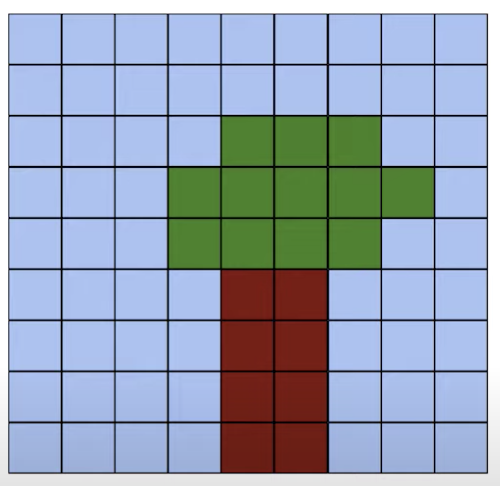
\includegraphics[height=0.35\textheight]{figures/image-tree.png}
  \end{center}
Input image.
\end{minipage}
\hspace{2mm}
\begin{minipage}{0.35\linewidth}
  \begin{center}
    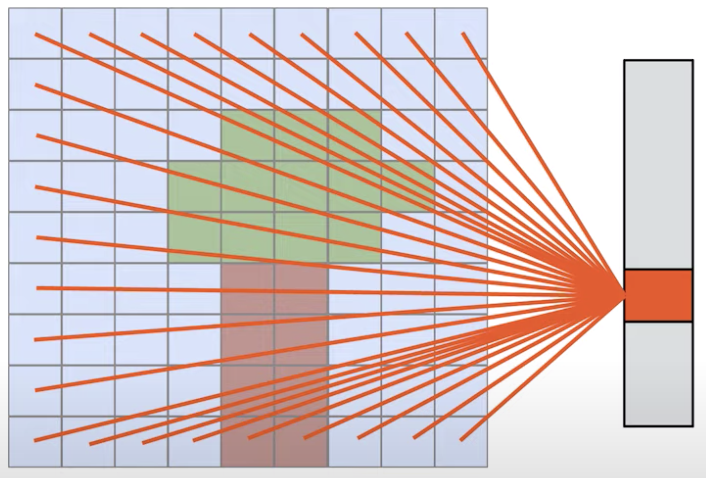
\includegraphics[height=0.35\textheight]{figures/fc-net.png}
  \end{center}
Fully connected layer.
\end{minipage}
\hspace{1mm}
\begin{minipage}{0.35\linewidth}
  \begin{center}
    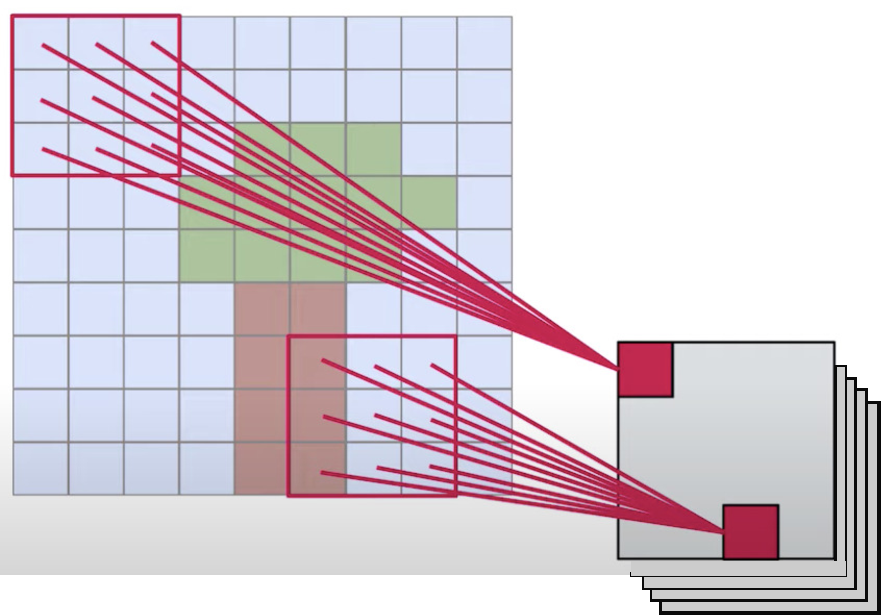
\includegraphics[height=0.4\textheight]{figures/convnet_v2.pdf}
  \end{center}
Convolutional layer.
\end{minipage}
\vfill
\scriptsize{Figures adapted from \citem{dieleman2020}.}\\
\vsp
\vsp
\normalsize{Check out more animated illustrations:}
\begin{itemize}
\item \link{https://github.com/vdumoulin/conv_arithmetic}\\
\item \link{https://cs231n.github.io/convolutional-networks/}
\end{itemize}
Also: lecture by Sander Dieleman (Deepmind) at UCL, London:
\link{https://www.youtube.com/watch?v=shVKhOmT0HE&feature=youtu.be}

\end{frame}

\begin{frame}{Convolutional layers, operation}
\vspace{-3mm}
Let $C$, $H$, $W$, $C'$, $H'$, $W'$, $d_{1}$, $d_{2}$ denote positive integers.\\
Description for 2D case. 2D convolutional layer:
\vsp
\begin{itemize}
\item \textbf{input}: image-like tensor $x$ with shape ($C$, $H$, $W$) (let's omit batch for now)
\item  \textbf{output}: also image-like $y$ with shape ($C'$, $H'$, $W'$), called \textit{feature map}
\item \textbf{model parameters}: weights and biases!
\begin{itemize}
\item ConvNets have $C'$ \emphbf{kernels}/\emphbf{filters} (vs.~Linear layers' weight matrix).
\item[-] $C'$ = number of output channels
\item Each kernel is a tensor of size ($C$, $d_{1}$, $d_{2}$). Here let's assume square kernels $d=d_1=d_2$. They are small ``image templates''.
\item bias $b \in \mathbb{R}^{C'}$ 
\end{itemize}
\end{itemize}
\vsp
\vsp
\pause
 Given \textbf{input} $x \in \mathbb{R}^{C \times H \times W}$, for each each output channel $ 1 \leq k \leq C'$, \textbf{output} $y_{k, i, j}$ ($ 1 \leq i \leq H'$, and $ 1 \leq j \leq W'$) is computed using the corresponding \textbf{kernel} $f^{(k)}$ of size $d$ (i.e.\, $f^{(k)} \in \mathbb{R}^{C \times d \times d}$):
\[
y_{k, i, j} =  \sigma\left(b_{k} + \sum_{c=1}^{C} \sum_{i'=i}^{i+d-1} \sum_{j'=j}^{j+d-1} f^{(k)}_{c, i'-i+1, j'-j+1} \times x_{c, i', j'}\right)
\]
\end{frame}

\begin{frame}{Convolutional layers, operation (cont'd)}
% Given \textbf{input} $x \in \mathbb{R}^{C \times H \times W}$, for each each output channel $ 1 \leq k \leq C'$, \textbf{output} $y_{k, i, j}$ ($ 1 \leq i \leq H'$, and $ 1 \leq j \leq W'$) is computed using the corresponding \textbf{kernel} $f^{(k)}$ of size $K$:
%\[
%y_{k, i, j} =  \sigma\left(b_{i,j} + \sum_{c=1}^{C} \sum_{i'=i}^{i+K-1} \sum_{j'=j}^{j+K-1} f^{(k)}_{c, i'-i+1, j'-j+1} \times x_{c, i', j'} \right)
%\]
\begin{itemize}
\item Indices make it look complicated, but it is not!\\
 We are sliding each kernel on the input image.\\
See e.g. \link{https://github.com/vdumoulin/conv_arithmetic/blob/master/gif/no_padding_no_strides.gif}
\item At each position, for each kernel, we are simply
computing the \textbf{dot product} (similarity measure) between the kernel and the input image within the local window.
\item Some terminologies: 
\begin{itemize}
\item[-] Locally connected (as opposed to fully connected)
\item[-] Weight sharing (across positions).
\end{itemize}
\item Note: computing a similarity between two ``vectors" using dot product is a fundamental concept (we will also see this for computing \textit{attention}). 
\end{itemize}
\end{frame}

\begin{frame}{Convolutional layers, specifications}
\vspace{-5mm}
To fully define the convolutional layer, we have to specify:
\begin{itemize}
\item number of input/output channels
\item kernel size
\item padding: how many "zeros" (or ones?) do we add on the borders to adjust the output ``image" size?\\
\link{https://github.com/vdumoulin/conv_arithmetic/blob/master/gif/same_padding_no_strides.gif}
\item stride: how many positions do we skip when we move the kernel over the image? also influence output size.\\
\link{https://github.com/vdumoulin/conv_arithmetic/blob/master/gif/padding_strides.gif}
\end{itemize}
See options in PyTorch \codeb{nn.Conv2d}. No need to overthink.
\begin{figure}
\centering
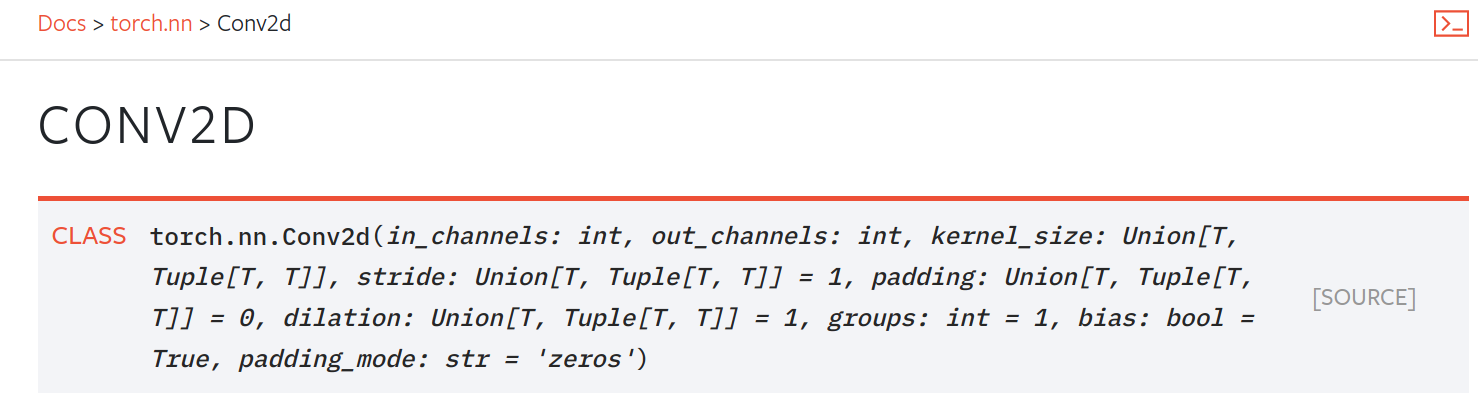
\includegraphics[width=.8\linewidth]{./figures/conv2d_pytorch.png}
\end{figure}
\end{frame}

\begin{frame}{More options in \codeb{nn.Conv2d} (excursion)}
\begin{itemize}
\item \code{groups}: number into which the input and output channels will be grouped.\\
Each group processed by different set of kernels.\\
\textit{grouped convolution (right)} with its equivalent with parallel convolution pipelines (left):
\begin{figure}
\centering
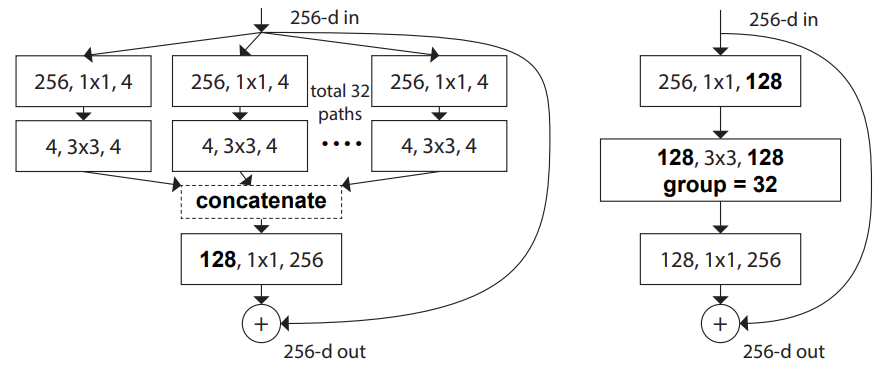
\includegraphics[width=.6\linewidth]{./figures/grouped_conv.png}
\end{figure}
Figure from \citem{XieGDTH17}. Idea used already in \citem{KrizhevskySH12}.
\vsp
\item \code{dilation}: spacing between kernel elements. For \textit{dilated convolution}.\\
See \link{https://github.com/vdumoulin/conv_arithmetic/blob/master/gif/dilation.gif}.
Got popular for audio processing \citem{oord2016wavenet}.
\end{itemize}
\end{frame}


%\begin{frame}{Convolutional neural networks,\\ recap jargon}
%\begin{itemize}
%\item Kernel\\
%(kernel is a quite overloaded term in ML...)
%\item Receptive field
%\item Feature map...
%\end{itemize}
%\end{frame}

\begin{frame}{Pooling layer}
 \vspace{-4mm}
\begin{itemize}
\item \textbf{input}: image $x$ with shape ($C$, $H$, $W$).
\item  \textbf{output}: also image $y$ with shape ($C'$, $H'$, $W'$). But smaller than $x$.
\item Operation: take max/mean over small, local sliding window to reduce image resolution (\emphbf{downsampling}).
\item \textbf{Allows to reduce computation for the following layer.}
\item \textbf{No model parameter}. Just a max/mean operation.
\item Hyper-parameter: as for convolution, need to specify pooling window dimensions, and how to move the window (stride).
\end{itemize}
\begin{figure}
                        \centering
                        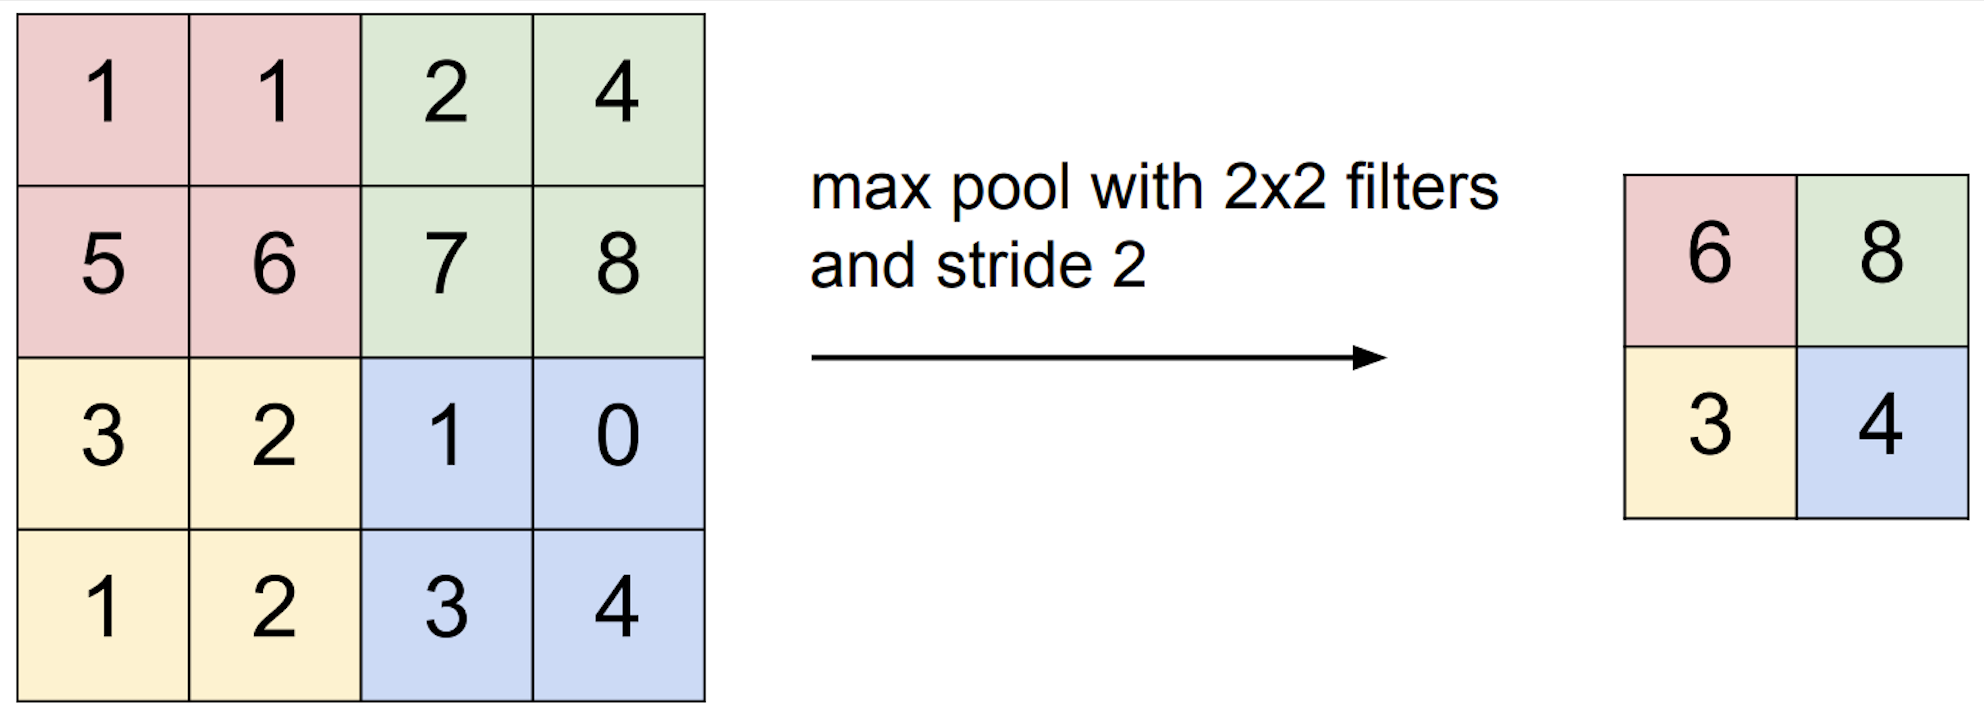
\includegraphics[width=.65\linewidth]{./figures/max-pool-better.png}
% \vspace{-3mm}
\end{figure}
\scriptsize{Figure taken from \citem{stanford2019cnn}.}
%For example, pooling by factor 2:
%\[
%y_{k, i, j} = \max_{\substack{ 2 * i \leq i' \leq 2 * (i+K-1),\\  j \leq 2 * j' \leq 2 * (j+K-1)}}  x_{k, i', j'}
%\]
%where $K$ is the window size. Check indices!
%Note: Convolutional layer (with stride $\geq 2$) can also do downsampling. Convolution can be learned, but max-pooling is cheaper.
\end{frame}

\begin{frame}[fragile]{PyTorch examples}
\begin{itemize}
\item \codeb{nn.Conv2d} layer:
\begin{itemize}
\item Check input/output \textbf{shapes}!
\end{itemize}
\end{itemize}
\begin{python}
>>> input = torch.randn(16, 3, 48, 48)  # (B, C, H, W)
>>> layer = nn.Conv2d(3, 32, 3)  # default padding=0
>>> layer.weight.shape
torch.Size([32, 3, 3, 3])
>>> layer.bias.shape
torch.Size([32])
>>> output = layer(input)
>>> output.size()
torch.Size([16, 32, 46, 46])
>>> layer = nn.Conv2d(3, 32, 3, padding=1)
>>> output = layer(input)
>>> output.size()
torch.Size([16, 32, 48, 48])
>>> # it's flexible:
>>> layer = nn.Conv2d(3, 32, (3, 5), stride=(2, 1), padding=(1, 2))
>>> output = layer(input)
>>> output.size()
torch.Size([16, 32, 24, 48])
\end{python}
\end{frame}

\begin{frame}[fragile]{PyTorch examples (cont'd)}
\begin{itemize}
\item Max pooling layer: \codeb{nn.MaxPool2d}
\end{itemize}
\begin{python}
>>> input = torch.randn(16, 3, 48, 48)  # (B, C, H, W)
>>> pooling = nn.MaxPool2d(3)
>>> # non-overlapping pooling w/ window size (3, 3)
>>> output = pooling(input)
>>> output.size()  # 48 / 3 = 16
torch.Size([16, 3, 16, 16]) 
>>> # overlapping pooling w/ stride (2, 2)
>>> pooling = nn.MaxPool2d(3, stride=2)
>>> output = pooling(input)
>>> output.size()
torch.Size([16, 3, 23, 23])
>>> pooling = nn.MaxPool2d(3, stride=2, padding=1)
>>> # same as stride=(2, 2), padding=(1, 1)
>>> output = pooling(input)
>>> output.size()
torch.Size([16, 3, 24, 24])
>>> # downsampling by a factor 2 using a window size 3.
\end{python}
\end{frame}


\begin{frame}[fragile]{Put them together}
\vspace{-5mm}
ConvNets are obtained by alternating convolutional and pooling layers:
\begin{python}
class ConvNet(nn.Module):
    def __init__(self):  # just example.
        super(ConvNet, self).__init__()
        self.conv1 = nn.Conv2d(3, 6, 5)  # input shape (3, 32, 32).
        self.pool = nn.MaxPool2d(2, 2)
        self.conv2 = nn.Conv2d(6, 16, 5)
        self.fc1 = nn.Linear(16 * 5 * 5, 128)
        self.fc2 = nn.Linear(128, 64)
        self.fc3 = nn.Linear(64, 10)  # 10 output classes.

    def forward(self, x):
        x = self.pool(F.relu(self.conv1(x)))  # conv, pool.
        x = self.pool(F.relu(self.conv2(x)))  # conv, pool.
        x = x.view(-1, 16 * 5 * 5)  # linearlize input "images".
        x = F.relu(self.fc1(x))  # fully connected.
        x = F.relu(self.fc2(x))  # fully connected.
        x = self.fc3(x)  # fully connected.
        return x
\end{python}
\end{frame}

% \begin{frame}{Convolutional neural networks,\\  variants}
% There are many extensions/variants to convolutional neural networks...
% \begin{itemize}
% \item Dilated convolution \citem{YuK15}
% \item Depthwise-separable convolution \citem{Chollet17}
% \item ...
% \end{itemize}
% \end{frame}

\begin{frame}{So, shall we put more layers?}
\begin{itemize}
\item Observation (all figures from \citem{HeZRS16slides}):
\end{itemize}
\begin{figure}
\centering
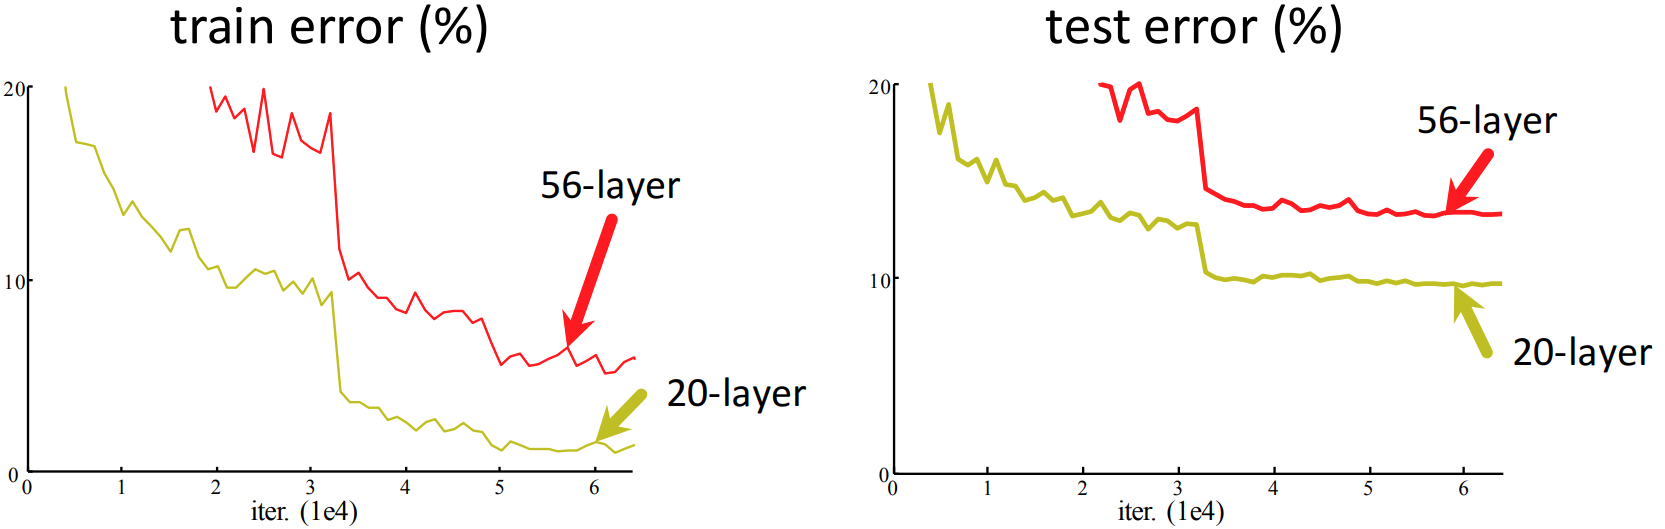
\includegraphics[width=.65\linewidth]{./figures/no_resnet.png}
\end{figure}
\begin{itemize}
\item More layers should never hurt? If they learn identity in the worst case!
\end{itemize}
\begin{minipage}{0.45\textwidth}
\begin{center}
    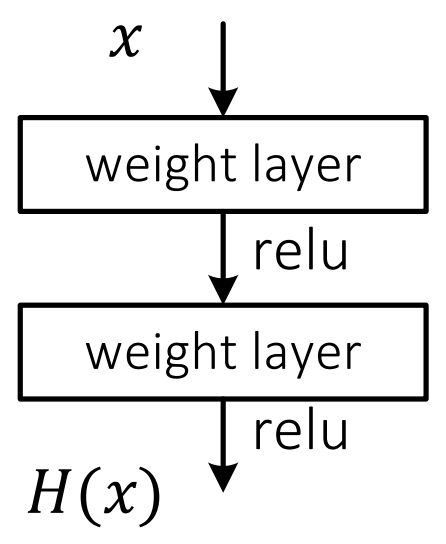
\includegraphics[height=0.35\textheight]{figures/plain_net.png} \\
Standard network.
\end{center}
\end{minipage}
\begin{minipage}{0.45\textwidth}
\begin{center}
    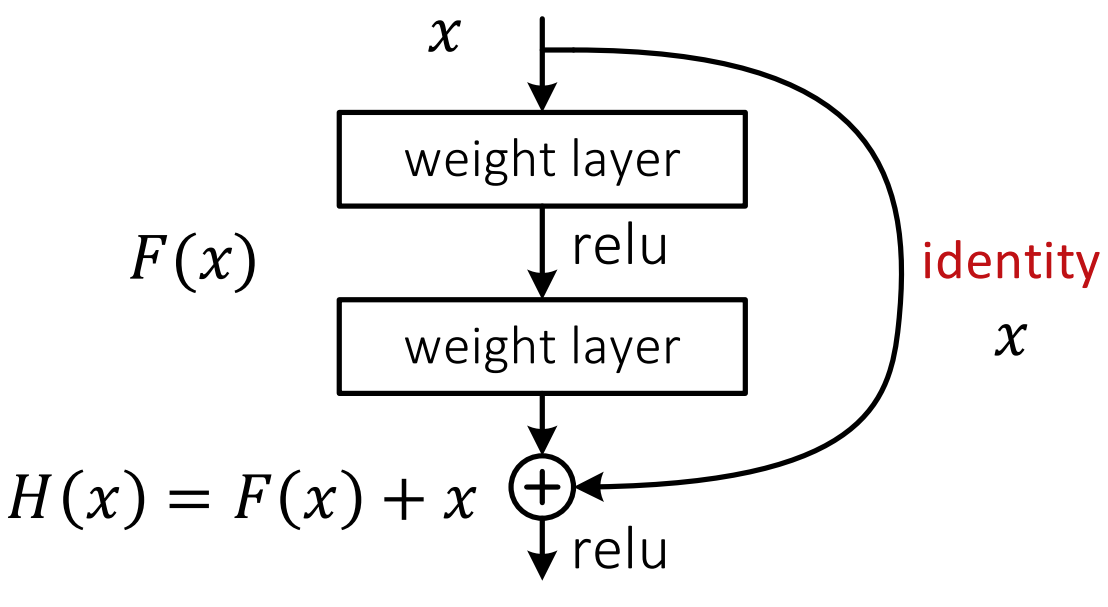
\includegraphics[height=0.3\textheight]{figures/resnet.png}\\
Residual block.
\end{center}
\end{minipage}
\vsp
\begin{itemize}
\item Alternative intuition: simply inspired by LSTM-RNN (up next!).
\end{itemize}
\end{frame}

\begin{frame}{Very Deep NNs with skip connections}
\begin{itemize}
\item \emphbf{Skip connections}:
if a layer applies transformation $F$ to $x$ to get $y = F(x)$,
directly ``connect" $x$ to $y$ by skipping the transformation.
\item Two types:
\begin{itemize}
\item  \emphbf{Highway connection/networks} \citem{NIPS2015_5850} from \textbf{IDSIA}.\\
Gated connection like in LSTM (next subsection!):\\
$y = F(x) \odot g(x)+ x \odot h(x) $, \\
where $\odot$ denotes element-wise multiplication and the \textit{gates} $g$ and $h$ are neural networks.\\
\item \emphbf{Residual connection/networks} \citem{HeZRS16}. \\
Simple addition:
$y = F(x) + x $
\end{itemize}
\end{itemize}
\hspace{-10mm}
{\raggedleft
    \includegraphics[height=0.09\textheight]{figures/deep_net.png} \\
}
\begin{itemize}
\item Enable training models with more than 1000 layers in image recognition.
\item Also used in Transformer architectures (see later...)
\end{itemize}
\end{frame}

\begin{frame}{Skip connections, performance}
\begin{itemize}
\item 
ImageNet Large Scale Visual Recognition Competition (ILSVRC) top-5 error (\%) (from \citem{HeZRS16slides}):
\end{itemize}
\begin{figure}
\centering
\includegraphics[width=.5\linewidth]{./figures/image_net.png}
\end{figure}
\begin{itemize}
\item Many follow up works... 
\begin{itemize}
\item By the same authors: improved resblocks \citem{HeZRS16b} (deeper)
\item Wide residual nets \citem{ZagoruykoK16}
\item DenseNets \citem{HuangLMW17, lang1988learning}...
\end{itemize}
\end{itemize}
\end{frame}

\begin{frame}{Convolutional neural networks,\\
beyond images}
\textbf{Applications beyond image processing}:
\begin{itemize}
\item Natural language: e.g.
\begin{itemize}
\item Text classification \citem{kim2014convolutional}
\item Machine translation \citem{GehringAGYD17}
\end{itemize}
\item Speech recognition \citem{waibel1989phoneme}
\end{itemize}\vsp
... and much more. We could have done the whole lecture on ConvNets...\\
\vsp
\textbf{From engineering view point,}
\begin{itemize}
\item Like pooling layers, convolutional layers (with stride $\geq 2$) allow us to downsample the input (reduce input resolution).
\item  It's a general tool for trainable downsampling (e.g.
reduce a long sequence to a shorter one).
\item Convolution can be learned vs. max-pooling is parameter-free and cheap.
\end{itemize}
Interested in historical background? Watch Prof. Schmidhuber's video: \link{https://youtu.be/ysOw6lNWx2o?t=20}
\end{frame}

\begin{frame}{Exercise 5 / Assignment 2}
	A few words on \emphbf{Assignment 2}:
	\begin{itemize}
		\item You will be building a full pipeline for image classification using
        \item[-] convolutional neural networks
        \item[-] some practical training tricks
		\item Remember the usual workflow (Chapter 1)!
        \item Similar task in Exercise 4
	\end{itemize}
\end{frame}

%%%%%%%%%%%%%% RNNs

\subsection{Recurrent NNs and LSTM}
\begin{frame}{Recurrent neural networks (RNNs)}
\vspace{-3mm}
\begin{itemize}
\item A neural network architecture for processing \textbf{sequences}.
\item[-] Consider a sequence of vectors $(x_1, x_2, ..., x_T)$ with $x_t \in \mathbb{R}^D$
\end{itemize}
\begin{itemize}
% \item RNNs have a \textbf{hidden state} $h_t \in \mathbb{R}^H$ which keep information about all past inputs until time $t$.
\item[-] \textbf{At each time step}, standard RNNs update its \textbf{hidden state} $h_t \in \mathbb{R}^H$ as a function of the \textbf{new input} $x_t$ and the \textbf{previous hidden states} $h_{t-1}$:
\[
h_t = f(W x_t + R h_{t-1} + b)
\]
where
\begin{itemize}
\item[-] $f$ is an activation function (e.g. $\tanh$)
\item[-] $W \in \mathbb{R}^{H \times D}$ and $R  \in \mathbb{R}^{H \times H}$
 are weight matrices, and $b \in \mathbb{R}^H$ a bias vector. 
\end{itemize}
\end{itemize}
\begin{figure}
                        \centering
                        \includegraphics[width=.25\linewidth]{./figures/rnn.pdf}
\end{figure}
\begin{itemize}
\item Initial state $h_0$: typically chosen to be zero.
\item Compression of \textbf{variable length context} $x_1, ..., x_{t}$ to a fixed size vector $h_t$.
% \item We can also stack multiple such layers to make the model deeper.
\end{itemize}
\end{frame}


\begin{frame}{Recurrent neural networks (cont'd)}
\begin{itemize}
\item \textbf{Conceptually}: two inputs, two linear transformations, then sum the results.
\[
h_t = f(W x_t + R h_{t-1} + b)
\]
\item Equivalent but better for efficient computation: \textbf{concatenate} the inputs, do \textbf{one} ``big" linear transformation.
\[
h_t = f( [W, R] 
      \begin{bmatrix}
           x_t \\
           h_{t-1} \\
         \end{bmatrix}
 + b)
\]
where $[W R] \in \mathbb{R}^{H \times (D+H)}$ and
$ \begin{bmatrix} x_t \\ h_{t-1} \\ \end{bmatrix} \in \mathbb{R}^{(D+H) \times 1}$ 
\item Look at the equation: it is just like the standard feedforward layer but with the previous output as a part of the input: recurrent.
\item (You typically do not need to do this concatenation explicitly; PyTorch takes care of it internally)
\end{itemize}
\end{frame}


\begin{frame}{Recurrent neural networks, example}
\vspace{-5mm}
\textbf{Language modeling}:
\vsp
\begin{itemize}
\item \textbf{Task}: given a word sequence $w_0, ..., w_{i-1}$, predict the next word $w_i$.
\item \textbf{input} to the network at each time step: previous word $w_{i-1} \in V$, where $V$ is the vocabulary.
\item \textbf{output}: probability distribution over the vocabulary $w \in V$: $p(w | w_0^{i-1})$.\\ (normalized vector of size $|V|$). NB: notation $w_0^{i-1} = (w_0, ..., w_{i-1})$
\item[-] RNN state $h_{i-1}$ compactly represents  all previous words $w_0^{i-1}$.
\item[-] Step-by-step computation:
\end{itemize}
\begin{figure}
                        \centering
                        \includegraphics[width=.65\linewidth]{./figures/rnn_lm.pdf}
\end{figure}
%\end{minipage}
\end{frame}

\begin{frame}{Embedding layer}
\vspace{-5mm}
\begin{itemize}
\item Neural networks process \textbf{vectors}.
\item Discrete input symbols (e.g. words) can be represented by \emphbf{one-hot} vectors.
\begin{itemize}
\item[-] The size of a one-hot vector is the vocabulary size.
\item[-] An ID is given to each word.
\item[-] One hot vector's entries are all 0 except at the position corresponding to its ID where it's 1.
\end{itemize}

\end{itemize}
\begin{figure}
\centering
\includegraphics[width=.7\linewidth]{./figures/emb.pdf}
\end{figure}
\vsp
\begin{itemize}
\item Matrix multiplication with a one-hot vector is a (column) \textbf{look-up} operation (try to write it down!).
\item[-] No need to do the actual multiplication. 
\item \emphbf{Embedding layer}: input = discrete ID, output: its vector representation (trainable parameters).
\item[-] Learning of the continuous representation (vector) of discrete tokens is part of the model.
\item[-] In PyTorch: \codeb{nn.Embedding}
\end{itemize}
\end{frame}


\begin{frame}{Recurrent neural networks, training}
\begin{itemize}
\item The most popular training algorithm: back-propagation \textit{through time}.
\item By unfolding the recurrence, we obtain a deep feed-forward neural network (see how many layers
are between $x_1$ and $h_4$ in the figure)
\item[-] You can apply back-propagation to the resulting network.
\item[-] One update of parameters given a sequence (a batch of sequences).
\end{itemize}
\begin{figure}
\centering
\includegraphics[width=.3\linewidth]{./figures/rnn.pdf}
\end{figure}
\vsp
\begin{itemize}
\item Unfolded model is as deep as the number of time steps. Typical problems:
\begin{itemize}
\item Exploding gradient
\item Vanishing gradient
\end{itemize}
\item Exploding gradient can be alleviated by \textit{clipping} gradient at some threshold (a hyper-parameter).
\end{itemize}

%\vsp
%Simple illustration by replacing $R$ by a scalar $0<\alpha<1$:\\
%\begin{itemize}
%\item[-] For each time step: the gradients are multiplied by $0<\alpha<1$. \\ $\rightarrow \alpha^2, \alpha^3,...$ get smaller (vanishing).\\
%\item[-] If $\alpha>1$, it gets larger (exploding).
%\item[-] Similar effect with matrices: having many matrix multiplications could attenuate gradients.
%\item[-] Exploding gradient can be alleviated by \textit{clipping} gradient at some threshold (hyper-parameter).
%\end{itemize}
\end{frame}

\begin{frame}[fragile]{Training, Batch, Padding}
\vspace{-5mm}
\begin{itemize}
\item How to create mini-batches to train RNNs?
\item Batch of shape e.g. (sequence length, batch size , feature dimension)
\item Sequences can have \emphbf{variable lengths}!
\end{itemize}
\vsp
We need to introduce \emphbf{padding}:
\begin{figure}
                        \centering
                        \includegraphics[width=.3\linewidth]{./figures/padding.pdf}
\end{figure}

\begin{itemize}
\item Add \textit{padding tokens} for short sequences such that all sequences get the same length (gray boxes above).
\item Run the RNN on the padded batch.
\item \textbf{Exclude the loss values from the padded positions}.\\
See for example \codeb{ignore\_index} argument in \codeb{nn.CrossEntropyLoss}.
\end{itemize}
\end{frame}

\begin{frame}{Truncated back-propagation through time}

\begin{itemize}
\item In some cases, sequences are too long for back-propagation through the entire sequence.
%\item In some cases, we would want to train RNNs to be evaluated/used for unlimited number of steps.
\item We typically use \emphbf{truncated} back-propagation through time.
%\item More we pad, more we waste computation...
%\item Trade-off: we can engineer it (e.g. sort sequences by lengths) but can lose model performance. 
%\item Or, if the nature of the problem allows it:
\begin{itemize}
\item Create fixed-length chunk/segments from the original sequences
by splitting/concatenating them.
\item \textbf{Carry over} the state vectors between two consecutive batches in the forward pass, but
\item Only propagate gradients \textbf{within} the batch in the backward pass.
\end{itemize}
\end{itemize}
% \vsp
\begin{figure}
                        \centering
                        \includegraphics[width=.5\linewidth]{./figures/truncated_bptt.pdf}
\end{figure}


\end{frame}


\begin{frame}{Other architectures, long short-term memory (LSTM) and gating}
\begin{minipage}{0.6\linewidth}
\vsp
Now look at this RNN:
\begin{itemize}
\item Three gates, input/forget/output gates (parameterized by an NN):
\vspace{-3mm}
    \begin{eqnarray*} 
    i_{t} &=& \sigma(W_{i} x_{t} + R_{i} h_{t-1} + b_i) \\
    f_{t} &=& \sigma(W_{f} x_{t} + R_{f} h_{t-1} + b_f) \\
    o_t &=& \sigma(W_{o} x_{t} + R_{o} h_{t-1} + b_o) 
    \end{eqnarray*}
\item Input candidate:
\vspace{-3mm}
    \begin{eqnarray*} 
    z_t &=&  \tanh(W_{z} x_{t} + R_{z} h_{t-1} + b_z) 
    \end{eqnarray*}
\item Update cell states using the input and forget gates:
\vspace{-3mm}
    \begin{eqnarray*} 
    c_{t} &=&  f_{t} \odot c_{t-1} + i_{t} \odot  z_t 
    \end{eqnarray*}
\item Output: $h_t = o_{t} \odot \tanh(c_t)$
%\vspace{-3mm}
%    \begin{eqnarray*} 
%    h_t &=& o_{t} \odot \tanh(c_t)
%    \end{eqnarray*}
\end{itemize}
\vsp
(layer index $(\ell)$ omitted in the equations.)
\end{minipage}
\begin{minipage}{0.39\linewidth}
\begin{figure}
                        \centering
                        \includegraphics[width=.9\linewidth]{./figures/lstm.pdf}
\end{figure}
\end{minipage}
\end{frame}


\begin{frame}{Long short-term memory and gating (cont'd)}
\begin{minipage}{0.55\linewidth}
Special RNN architecture to alleviate vanishing gradient \citem{hochreiter1997long, gers2000learning}.
\begin{itemize}
\item two hidden state vectors
\item internal cell state with an additive connection over time (no multiplication with a weight matrix! good gradient flow).
\item \textbf{differentiable/soft multiplicative gates} (input/forget/output gates) control information flow around the cell
\item each gate parameterized by a neural network.
\end{itemize}
Inspired many other new architectures!
\end{minipage}
\begin{minipage}{0.4\linewidth}
\begin{figure}
                        \centering
                        \includegraphics[width=.9\linewidth]{./figures/lstm.pdf}
\end{figure}
\end{minipage}
\end{frame}
%
%\begin{frame}{Long short-term memory and gating}
%\begin{minipage}{0.6\linewidth}
%\vsp
%\begin{itemize}
%\item Three gates (parameterized by NN):
%\vspace{-3mm}
%    \begin{eqnarray*} 
%    i_{t} &=& \sigma(W_{i} x_{t} + R_{i} h_{t-1} + b_i) \\
%    f_{t} &=& \sigma(W_{f} x_{t} + R_{f} h_{t-1} + b_f) \\
%    o_t &=& \sigma(W_{o} x_{t} + R_{o} h_{t-1} + b_o) 
%    \end{eqnarray*}
%\item Input candidate:
%\vspace{-3mm}
%    \begin{eqnarray*} 
%    z_t &=&  \tanh(W_{z} x_{t} + R_{z} h_{t-1} + b_z) 
%    \end{eqnarray*}
%\item Update cell states using input and forget gates:
%\vspace{-3mm}
%    \begin{eqnarray*} 
%    c_{t} &=&  f_{t} \odot c_{t-1} + i_{t} \odot  z_t 
%    \end{eqnarray*}
%\item Output: $h_t = o_{t} \odot \tanh(c_t)$
%%\vspace{-3mm}
%%    \begin{eqnarray*} 
%%    h_t &=& o_{t} \odot \tanh(c_t)
%%    \end{eqnarray*}
%\end{itemize}
%\vsp
%(layer index $(\ell)$ omitted in the equations.)
%\end{minipage}
%\begin{minipage}{0.39\linewidth}
%\begin{figure}
%                        \centering
%                        \includegraphics[width=.9\linewidth]{./figures/lstm.pdf}
%\end{figure}
%\end{minipage}
%\end{frame}

\begin{frame}{Long short-term memory and gating\\ (cont'd)}
\begin{itemize}
\item Again, linear transformations can be grouped.
\vspace{-3mm}
    \begin{eqnarray*}
      \begin{bmatrix}
           i_t \\
           f_t \\
           o_t \\
           z_t \\
         \end{bmatrix}
= 
      \begin{bmatrix}
           \sigma \\
           \sigma \\
           \sigma \\
           \tanh \\
         \end{bmatrix}
      \begin{bmatrix}
           W_{i}, R_{i} \\
           W_{f}, R_{f} \\
           W_{o}, R_{o} \\
           W_{z}, R_{z} \\
         \end{bmatrix} 
      \begin{bmatrix}
           x_t \\
           h_{t-1} \\
         \end{bmatrix}
+ 
      \begin{bmatrix}
           b_i \\
           b_f \\
           b_o \\
           b_z \\
         \end{bmatrix}
    \end{eqnarray*}
\item The rest as in the previous slide:
    \begin{eqnarray*}
    c_{t} &=&  f_{t} \odot c_{t-1} + i_{t} \odot  z_t \\
    h_t &=& o_{t} \odot \tanh(c_t)
    \end{eqnarray*}
%\vspace{-3mm}
%    \begin{eqnarray*}
%    h_t &=& o_{t} \odot \tanh(c_t)
%    \end{eqnarray*}
\end{itemize}
\vsp
NB: $      \begin{bmatrix}
           W_{i}, R_{i} \\
           W_{f}, R_{f} \\
           W_{o}, R_{o} \\
           W_{z}, R_{z} \\
         \end{bmatrix} \in \mathbb{R}^{4H \times (D+H)}$ and  
$\begin{bmatrix}
           b_i \\
           b_f \\
           b_o \\
           b_z \\
         \end{bmatrix} \in \mathbb{R}^{4H \times 1}$
\end{frame}



\begin{frame}{Recurrent neural networks, implementations}
\textbf{Two types} of RNN \emphbf{implementations}:
\begin{itemize}
\item \emphbf{Step-by-step} RNN functions:
\begin{itemize}
\item take one input, output one output.
\item expect you to write the loop over sequence. 
\item e.g. \codeb{torch.nn.LSTMCell}
\end{itemize}
\item \emphbf{Entire sequence} RNN functions:
\begin{itemize}
\item take sequence, output sequence
\item e.g. \codeb{torch.nn.LSTM}
\end{itemize}
\item In general: you should use the entire sequence one whenever you can,
which is optimized/faster.\\
\item[-] High-level spirit: use built-in code as much as possible (avoid your own plain code in Python).\\
% \item Some simple optimization possible (without C++) using TorchScript?
\end{itemize}
\end{frame}

\begin{frame}[fragile]{Recurrent neural networks, implementations (cont'd)}
Sequence-level function:
\begin{python}
>>> rnn = nn.LSTM(10, 20, 2)  # in_dim, out_dim, num_layers
>>> inputs = torch.randn(6, 3, 10)  # (len, B, in_dim)
>>> h0 = torch.randn(2, 3, 20)  # (num_layers, B, out_dim)
>>> c0 = torch.randn(2, 3, 20)  # (num_layers, B, out_dim)
# outputs of shape (len, B, out_dim)
>>> outputs, (hn, cn) = rnn(inputs, (h0, c0))
>>> outputs.size()
torch.Size([6, 3, 20])
\end{python}
NB:
\begin{itemize}
\item Only possible if all inputs are known (for example in training, or in some evaluation setups).
\item If the input also depends on the previous time steps (for example during \textit{search}; we will see later)
we have no other choice but to go step by step.
\end{itemize}
\end{frame}

\begin{frame}[fragile]{Recurrent neural networks, implementations (cont'd)}
Step-by-step function:
\begin{python}
>>> rnn = nn.LSTMCell(10, 20)  # in_dim, out_dim
>>> input = torch.randn(6, 3, 10)  # (len, B, in_dim)
>>> h = torch.randn(3, 20)  # (B, out_dim)
>>> c = torch.randn(3, 20)  # (B, out_dim)
>>> output = []
>>> for i in range(6):  # "manual" Python loop
        h, c = rnn(input[i], (h, c))
        output.append(h)
>>> output = torch.stack(output, 0)  # from list to tensor
>>> output.size()
torch.Size([6, 3, 20])
\end{python}
\end{frame}


\begin{frame}[fragile]{Example toy task: $N$-back}
Task:
\begin{itemize}
\item Input: sequence of numbers (between 0 and $k-1$).
\item Target at each position: 1 if the current input is equal
to the number at the $n$-th position back. 0 otherwise.
\item Sequences can have different lengths.
\end{itemize}
\vsp
\begin{figure}
                        \centering
                        \includegraphics[width=.4\linewidth]{./figures/nback.pdf}
\end{figure}
\end{frame}

\begin{frame}[fragile]{Example toy task: $N$-back, model}
It is a binary classification at each position over a sequence.\\
Model:
\begin{itemize}
\item Read the input sequences using RNN.
\item Input: number between 0 and $k$ $\rightarrow$ discrete!
\item Actual input to the model: one hot representation: vector of size $k$
with zero entry everywhere except the position (embedding layer is not needed though: $k$ is small)
\item A classifier linear layer which maps the RNN's hidden vector to the
two output nodes (2 classes here; strictly speaking, one node is enough).
\item Cross entropy loss for training.
\end{itemize}
\end{frame}

%\begin{frame}[fragile]{Padding}
%
%\begin{itemize}
%\item The sequences can have different lengths!
%\end{itemize}
%\vsp
%We need to introduce \emphbf{padding}:
%\begin{itemize}
%\item How to construct batches with sequences of variable lengths?
%\item Add padding tokens (-1 for example) for short sequences such that
%all sequences get the same length.
%\item Run the RNN over the batch, and exclude padded positions from the loss computation.
%\item Note: more we pad, more we waste computation...
%\end{itemize}
%\end{frame}

\begin{frame}[fragile]{$N$-back, data generation}
\begin{itemize}
\item A helper function first:
\end{itemize}
\begin{python}
def nback(n, k, length, random_state):
  xi = random_state.randint(k, size=length)
  yi = np.zeros(length, dtype=int)

  for t in range(n, length):
    yi[t] = (xi[t-n] == xi[t])

  return xi, yi
\end{python}

\end{frame}

\begin{frame}[fragile]{$N$-back, data generation (cont'd)}
\vspace{-5mm}
\begin{itemize}
\item Main data generator:
\end{itemize}
\begin{python}
def create_dataset_nback(n_sequences, mean_length, std_length,
                         n, k, random_state):
  X, Y, lengths = [], [], []
  for _ in range(n_sequences):
    length = random_state.normal(loc=mean_length, scale=std_length)
    length = int(max(n+1, length))
    xi, yi = nback(n, k, length, random_state)
    X.append(xi)
    Y.append(yi)
    lengths.append(length)
  max_len = max(lengths)

  # We pad X w/ 0 (for one-hot), and Y w/ -1 (CE loss).
  X_arr = np.zeros((n_sequences, max_len), dtype=np.int64)
  Y_arr = np.zeros((n_sequences, max_len), dtype=np.int64) - 1

  for i in range(n_sequences):
    X_arr[i, 0: lengths[i]] = X[i]
    Y_arr[i, 0: lengths[i]] = Y[i]

  return X_arr, Y_arr, lengths
\end{python}

\end{frame}

\begin{frame}[fragile]{$N$-back, data generation (cont'd)}
\begin{itemize}
\item Generate data:
\end{itemize}
\begin{python}
import numpy as np

seed = 0
n = 3
k = 4
mean_length = 20
std_length = 5
n_sequences = 1000

random_state = np.random.RandomState(seed=seed)

X_train, Y_train, length_train = create_dataset_nback(
    n_sequences, mean_length, std_length, n, k, random_state)

X_val, Y_val, length_val = create_dataset_nback(
    n_sequences, mean_length, std_length, n, k, random_state)
\end{python}

\end{frame}

\begin{frame}[fragile]{$N$-back, RNN model}
\begin{itemize}
\item Create model: an RNN + a linear classifier layer.
\end{itemize}
\begin{python}
import torch.nn as nn

input_dim = 4
hidden_size = 64
num_layers = 1
num_classes = 2

rnn = nn.RNN(input_dim, hidden_size, num_layers)
linear = nn.Linear(hidden_size, num_classes)
h0 = torch.zeros(num_layers, n_sequences, hidden_size)  # init state
\end{python}

\begin{python}
import torch.optim as optim
# Again: alternatively write a model class!
params = list(rnn.parameters()) + list(linear.parameters())
optimizer = optim.Adam(params, lr=0.01)

# Exclude padded position (position with -1).
loss_fn = nn.CrossEntropyLoss(ignore_index=-1)
\end{python}
% loss_fn = nn.CrossEntropyLoss(ignore_index=-1, size_average=True) 
\end{frame}

\begin{frame}[fragile]{$N$-back, prepare data}
\begin{itemize}
\item Prepare data in the form/shape expected by RNNs:
\end{itemize}
\begin{python}
# prepare data
X = torch.from_numpy(X_train)
X = torch.nn.functional.one_hot(X)  # (B, len, k)
X = X.transpose(0, 1) 
X = X.float()

y = torch.from_numpy(Y_train)
y = y.transpose(0, 1).flatten()

# same for val:
X_val = torch.from_numpy(X_val)
X_val = torch.nn.functional.one_hot(X_val)
X_val = X_val.transpose(0, 1).float()
y_val = torch.from_numpy(Y_val).transpose(0, 1).flatten()
\end{python}

\end{frame}


\begin{frame}[fragile]{$N$-back, training}
\vspace{-5mm}
\begin{python}
num_train_steps = 200

total_val = sum(length_val)
total_tr = sum(length_train)

for step in range(num_train_steps):
  # more convenient if you had defined a model!
  # Please fix this in the exercise 6!
  rnn.train()
  linear.train()

  optimizer.zero_grad()
  output, hn = rnn(X, h0)
  output = output.view(-1, hidden_size)  # (B*len, dim)
  output = linear(output)

  loss = loss_fn(output, y)
  print(f"training loss: {loss}")

  loss.backward()
  optimizer.step()

# ... continue to the next slide ...

\end{python}

\end{frame}

\begin{frame}[fragile]{$N$-back, training (cont'd)}
\vspace{-5mm}
\begin{python}
# ... continue from the previous slide ...
  rnn.eval()
  linear.eval()  # more convenient if you had defined a model!
  with torch.no_grad():
    # Here evaluate also on training set (exercise 6).

    output_val, hn_val = rnn(X_val, h0)
    output_val = output_val.view(-1, hidden_size)
    output_val = linear(output_val)

    _, predicted_val = outputs_val.max(dim=1)
    correct_val = (predicted_val == y_val)

    # Important: do not count padded position!!
    mask_val = (y_val >= 0)
    correct_val = (correct_val * mask_val).sum().item()

    print(f'epoch: {step}, val acc: {100 * correct_val / total_val}')
\end{python}
\end{frame}


%\begin{frame}[fragile]{$N$-back, training (cont'd)}
%\vspace{-5mm}
%\begin{python}
%# ... continue from the previous slide ...
%  rnn.eval()
%  linear.eval()  # more convenient if you had defined a model!
%  with torch.no_grad():
%    output_tr, hn_tr = rnn(X, h0)
%    output_tr = output_tr.view(-1, hidden_size)
%    output_tr = linear(output_tr)
%    _, predicted_tr = outputs_tr.max(dim=1)
%    correct_tr = (predicted_tr == y)
%    mask_tr = (y >= 0)  # Important: do not count padded position!!
%    correct_tr = (correct_tr * mask_tr).sum().item()
%    print(f'epoch: {step}, train acc: {100 * correct_tr / total_tr}')
%
%    output_val, hn_val = rnn(X_val, h0)
%    output_val = output_val.view(-1, hidden_size)
%    output_val = linear(output_val)
%    _, predicted_val = outputs_val.max(dim=1)
%    correct_val = (predicted_val == y_val)
%    mask_val = (y_val >= 0)
%    correct_val = (correct_val * mask_val).sum().item()
%    print(f'epoch: {step}, val acc: {100 * correct_val / total_val}')
%\end{python}
%
%\end{frame}


\begin{frame}{Preview:\\ Exercise 6 \& Exercise 7 / Assignment 3}
	Both \emphbf{Exercise 6} and \emphbf{Exercise 7 / Assignment 3}
	\begin{itemize}
		\item Introduction to language modeling with RNNs
	\end{itemize}
\end{frame}

\begin{frame}{Preliminaries for Assignment 3,\\ Reminders}
\begin{minipage}{0.6\linewidth}
\begin{itemize}
\item Language models compute $p(w_i | w_0^{i-1})$ Notation: $w_0^{i-1} = (w_0, w_1, ..., w_{i-2}, w_{i-1})$
\item Given a sentence $w_1^N$,\\
$\displaystyle p(w_1, ..., w_N) = \prod_{i=1}^{N} p(w_i | w_0^{i-1})$
where\\ $w_0$ denotes an artificial start symbol
\item This can be used to compute probabilities of sentences,
e.g., which sentence should get a higher probability?
\begin{itemize}
\item[-] $p(\text{I hate cars \texttt{<eos>}})$
\item[-] $p(\text{I ate cars \texttt{<eos>}})$
\end{itemize}
where \texttt{<eos>} is the end-of-sentence token.
\item Another application in this assignment: text completion/generation.
\end{itemize}
\end{minipage}
\begin{minipage}{0.35\linewidth}
\begin{figure}
\centering
\includegraphics[width=1.\linewidth]{./figures/lm.pdf}
\end{figure}
\end{minipage}
\end{frame}

\begin{frame}{Preliminaries for Assignment 3}
\begin{itemize}
\item This \textbf{assignment}: text generation/completion.\\
\item[-] Once the model is trained, you will provide a beginning of some text $w_0^{i-1}$.
\item[-] You let the model complete your text.\\
You: \texttt{Dogs like best to}\\
Your LM: \texttt{eat , play , and sleep}
\end{itemize}
\vsp
\pause
How can this be done?
\pause
\begin{itemize}
\item Given the beginning of a sentence $w_0^{n-1}$,
let your LM compute $p(. | w_0^{n-1})$ (i.e., the probability distribution over the \textbf{next} word/token)
\item Then there are 2 possibilities:
\item[-] (1) Take the word with the highest probability. $\hat{w} = \argmax_w p(w | w_0^{n-1})$
\item[-] (2) Randomly sample $\hat{w}$ from the distribution $p(w | w_0^{n-1})$
\item Then feed the chosen word $\hat{w}$ to the LM as an input, and continue for a fixed number of steps.
\end{itemize}
\end{frame}

\begin{frame}{Preliminaries for Assignment 3,\\
Sampling vs. Search.}
\begin{itemize}
\item \emphbf{Search}: we want to find the most likely output from the model.
\item[-] In the assignment, \textbf{greedy search}:
\begin{itemize}
\item At each time step, obtain the most likely token.
\end{itemize}
\item \emphbf{Sampling}: we want to generate diverse outputs from the model.
\begin{itemize}
\item Randomly sample according to the model's output distribution.
\end{itemize}
In both cases, use the corresponding model output token as the input to the model for the next time step.
\end{itemize}
\end{frame}

\begin{frame}{Preliminaries for Assignment 3,\\
Pre-processing/Tokenization}
The data is a plain text file.
\begin{itemize}
\item The modeling unit must be defined: the text must be \textbf{tokenized}, e.g.
\item[-] Word level: i.e. split the text by white space.
\item[-] Character level
\end{itemize}
\vsp
Side note (not needed for A3): in general, depending on the task,
we also have to do some text pre-processing:
\begin{itemize}
\item[-] Normalization of lower/upper case, numbers, punctuations, or spelling, remove strings which are not really texts, etc.
\end{itemize}
\emphbf{Vocabulary} of the model:
\begin{itemize}
\item Add all characters found in the training set.
\item Add \textbf{special} tokens: pad token, unknown token, end-of-sentence token (not needed for A3), ...
\end{itemize}
See the helper code available on iCorsi.
\end{frame}
%


\subsection{Attention, Self-attention, Transformers}
\begin{frame}[fragile]{Illustration first!}
\vspace{-5mm}
\begin{python}
>>> dict = {'apple': 4, 'banana': 2, 'orange': 5}  # fruit counts
>>> dict.keys()
dict_keys(['apple', 'banana', 'orange'])
>>> dict.values()
dict_values([4, 2, 5])
>>> dict['orange']  # query 'orange'
5
\end{python}
\begin{itemize}
\item A dictionary \emphbf{stores} \emphbf{key} and \emphbf{value} pairs.
\item Retrieval: the \emphbf{query} (here \code{orange}) is \emphbf{compared} to the keys,
and the value corresponding to the matching key is returned.
\end{itemize}
\pause
\vsp
\textbf{Can we do this in a differentiable way using neural networks?}
\pause
\begin{itemize}
\item \textbf{How to handle symbols?} Reminder from the last lecture: replace each symbol (key, query, value) by its vector representation.
\pause
\item \textbf{How to compare query and key?} E.g., compute the dot product between query and key vectors.
\pause
\item \textbf{How to output the value of the matching key (in a differentiable way)?} Return the \textit{weighted sum} of all value vectors where weights are the key/query similarity scores.
\end{itemize}
\end{frame}

\begin{frame}{Attention with neural networks}
% \vspace{-5mm}
\begin{itemize}
\item Two lists of $N$ vectors each, with dimensions $d_{\text{key}}$ and $d_{\text{value}}$\\
\begin{itemize}
\item \emphbf{keys} $\mathcal{K} = (k_1, ..., k_N) \in \mathbb{R}^{d_{\text{key}} \times N}$ \\
\item \emphbf{values} $\mathcal{V}=(v_1, ..., v_N) \in \mathbb{R}^{d_{\text{value}} \times N}$\\
\end{itemize}
\item One vector $q \in \mathbb{R}^{d_{\text{key}} \times 1}$ (called \emphbf{query}).\\
\end{itemize}
% \vsp
% Terminology \textit{query}, \textit{key}, \textit{value}: analogy of \textbf{retrieval in database}.\\
\pause
\vspace{1mm}
Between each \emphbf{key} vector $k_{i}$ with $1 \leq i \leq N$ and the \emphbf{query} vector $q$, the \textit{similarity} score $s_{i} \in \mathbb{R}$ is computed as:
      \begin{eqnarray*}
              s_{i}&=& k_{i}\bullet q\text{\hspace{12mm} $\bullet$ denotes the dot product.}
      \end{eqnarray*}
% \vspace{2mm}
\pause
This yields a similarly score vector $s \in \mathbb{R}^{N}$ that is then re-normalized to $\alpha = (\alpha_{1}, .., \alpha_{i}, .., \alpha_{N}) \in \mathbb{R}^{N}$ by:
      \begin{eqnarray*}
              \alpha &=& \softmax(s) \text{\hspace{3.5mm} where \hspace{1mm}} s = (s_{1}, .., s_{i}, .., s_{N}) \in \mathbb{R}^{N}.
      \end{eqnarray*}
% \vspace{3mm}
\pause
These scores are used to compute the \emphbf{weighted average} of \emphbf{value} vectors $v_{i}$:
      \begin{eqnarray*}
              \Attention(\mathcal{K}, \mathcal{V}, q) &=& \sum_{i=1}^{N} \alpha_{i} v_{i}.
      \end{eqnarray*}
\end{frame}

\begin{frame}{Attention with neural networks, comments}
\begin{itemize}
\item These operations can be written as matrix operations:
      \begin{eqnarray*}
              \Attention(\mathcal{K},\mathcal{V}, q) = \mathcal{V} \softmax(\mathcal{K}^{\intercal}q)
      \end{eqnarray*}
\vspace{-3mm}
\pause
\item A high attention score $\alpha_i$ indicates the \emphbf{attention} focused on the content ($k_i$,$v_i$) when the input is $q$, that is something we can visualize.
% Consider
% \vspace{-3mm}
\begin{figure}
                        \centering
                        \includegraphics[width=0.35\linewidth]{./figures/bahdanau_att.png}
\end{figure}
{\scriptsize Figure taken from \citem{bahdanau2014neural} for illustration.\\
We will see the English to French translation model in the next section.}
\end{itemize}
\end{frame}

\begin{frame}{Attention computation}
\vspace{-3mm}
There are various ways to compute the similarity scores $\simi(q, k) \in \mathbb{R}$
between two vectors $q, k \in \mathbb{R}^{d \times 1}$:
\begin{itemize}
\item dot attention \citem{luong-etal-2015-effective}
\[
\simi(q, k) = q \bullet k = q^{\intercal} k
\]
\pause
\item scaled dot attention \citem{trafo}
\[
\simi(q, k) = \dfrac{q^{\intercal} k}{\sqrt{d}}
\]
\pause
{\small ($\sqrt{d}$ because if elements in $q$ and $k$ are i.i.d random variables with mean 0 and variance 1, $q^{\intercal} k$ has mean 0 and variance $d$.)}
\pause
\item MLP attention \citem{bahdanau2014neural}
\[
\simi(q, k) = w^{\intercal} \tanh(W [q, k] + b)
\]
where $W \in \mathbb{R}^{d \times 2d}$ and $w, b \in \mathbb{R}^{d \times 1}$ are trainable parameters.
\end{itemize}
%\begin{itemize}
%\item scaled dot attention works well while being \textbf{efficient} (simple dot product!).
%\item \emphbf{Multi-head attention} is often used.
%\begin{itemize}
%\item[-] Carry out multiple attention operations using separate parameters, and concatenate the results from each head.
%\item[-] \code{torch.nn.MultiheadAttention}
%\end{itemize}
%\end{itemize}
\end{frame}

\begin{frame}{Attention computation (cont'd)}
In practice:
\begin{itemize}
\item \textbf{Scaled dot attention} works well while being efficient, and it has no parameter.
\item \emphbf{Multi-head attention} is often used:
\begin{itemize}
\item[-] Split each of key/value/query vectors into $H$ sub-vectors. $H$ is the number of heads.
\item[-] Compute separate attention operations for each key/value/query sub-vectors.
\item[-] Concatenate (feature dimension) the results from each head to get the final output.
\end{itemize}
e.g., if the dimension is 512 (for each of key, value and query), and we use 8 attention \textbf{heads}, each attention computation is carried out for 64 dimensional sub-vectors.
\item \code{torch.nn.MultiheadAttention}
\end{itemize}
%\begin{itemize}
%\item scaled dot attention works well while being \textbf{efficient} (simple dot product!).
%\item \emphbf{Multi-head attention} is often used.
%\begin{itemize}
%\item[-] Carry out multiple attention operations using separate parameters, and concatenate the results from each head.
%\item[-] \code{torch.nn.MultiheadAttention}
%\end{itemize}
%\end{itemize}
\end{frame}



\begin{frame}{Attention with neural networks, applications}
\begin{itemize}
\item Originally proposed for machine translation (next section).
\item Intuition: focus only on parts of the input sentence, while producing parts of target sentence...
\item Impact on many other applications: attention is everywhere now.
\item \emphbf{Differentiable implementation of dictionary/database retrieval}.
\item Fundamental idea of \emphbf{ignoring irrelevant information}.
\item Visualization and interpretability.
\end{itemize}
% We will see more concrete examples later, and in the \emphbf{final exercise/assignment}.
\end{frame}



\begin{frame}{Self-attention\\ (autoregressive version)}
Can we build a general purpose sequence processing layer based on attention?
\begin{itemize}
\item Alternative to RNNs to process sequences.
\pause
\item {\small Note: autoregressive means that we process a sequence $x_1^N$ from left to right (or right to left) step by step:
i.e. while predicting a token $x_n$, we make use of information from the past $x_1^{n-1}$.}
\pause
\item Basic idea: ``enlarge the database for each new input"\\
\begin{itemize}
\item[-] Each input transformed in 3 ways: key, value, and query vectors.
\item[-] Store key and value vectors from all predecessor inputs (``database")
\item[-] Compute the output via attention using the query vector.
\end{itemize}
\pause
\item Does this make sense?
\end{itemize}
%\pause
%\vspace{3mm}
%Result of incremental refinements:
%\begin{itemize}
%\item \cite{cheng16}: Proposed as augmentation for LSTM
%\item \cite{ParikhT0U16}: Generic formulation.
%\item \cite{trafo}: Used in multiple layers in Transformer.
%\end{itemize}
\end{frame}

\begin{frame}{Self-attention, illustration}
\begin{figure}
\hspace{-10mm}
                        \centering
                        \includegraphics[width=.7\linewidth]{./figures/self_attention_only.pdf}
\end{figure}
\begin{itemize}
\item \textbf{Abandon compression} ability of RNNs!
\item Perform very well as a part of \emphbf{Transformer} models (up next).
\end{itemize}
\end{frame}

\begin{frame}{Self-attention (cont'd)}
\begin{itemize}
\item Consider a sequence of vectors ($x_1$, ..., $x_N$):
\pause
\item At step $n$, input $x_n \in \mathbb{R}^{D \times 1}$ is first projected into \emphbf{three} vectors:
   \begin{eqnarray*}
q_n, k_n, v_n = Qx_n, Kx_n, Vx_n \text{\hspace{8mm}} Q,K \in \mathbb{R}^{d_{\text{key}} \times D}, V \in \mathbb{R}^{d_{\text{value}} \times D}
    \end{eqnarray*}
$Q,K,V$ are the \emphbf{trainable parameters} of the layer.
\pause
\item The \emphbf{memory} of the layer consists of \emphbf{concatenation} of $k_i$ and $v_i$ vectors (along position/time dimension)
for all predecessor inputs. Thus, at step $n$:

\begin{eqnarray*}
\mathcal{K}_n &=& \Concat\!\big(\mathcal{K}_{n-1}, k_n) \in \mathbb{R}^{d \times n} \\
\mathcal{V}_n &=& \Concat\!\big(\mathcal{V}_{n-1}, v_n) \in \mathbb{R}^{d \times n} \\
\end{eqnarray*}
%which is:
%\begin{eqnarray*}
%h_n = \big(\mathcal{K}_n, \mathcal{V}_n\big) = \big((\mathcal{K}_{n-1}, k_n), (\mathcal{V}_{n-1}, v_n)\big)
%\end{eqnarray*}


%   \begin{eqnarray*}
%h_n = \big(\mathcal{K}_n, \mathcal{V}_n\big) = \big((\mathcal{K}_{n-1}, k_n), (\mathcal{V}_{n-1}, v_n)\big)
%    \end{eqnarray*}
\pause
State size $h_n = \big(\mathcal{K}_n, \mathcal{V}_n\big)$ increases with the sequence length; unlike in RNNs!
\pause
\item Output $y_n $ is computed by \emphbf{attention} using these vectors:
   \begin{eqnarray*}
y_n = \SelfAttention(h_{n-1},x_n) = \Attention(\mathcal{K}_n, \mathcal{V}_n, q_n)
    \end{eqnarray*}
\end{itemize}
\end{frame}

\begin{frame}{Self-attention, positional encoding}
\vspace{-4mm}
\begin{itemize}
\item One more concept needs to be introduced: \emphbf{positional encoding}.
\item Attention operation is invariant to shuffling key-value pairs \{($k_i$, $v_i$)\}$_{1 \leq i \leq N}$.
\item[-] Positional information needs to be provided explicitly.
\item[-] Positional encoding is a vector of the same size as input word/token embeddings,
representing the position.
\item We \textbf{add} the positional encoding vectors to the input embeddings.
\end{itemize}
\end{frame}

\begin{frame}{Self-attention, positional encoding (cont'd)}
\begin{itemize}
\item Common model: \emphbf{sinusoidal positional encoding}.\\ $e(i) \in \mathbb{R}^D$ representing the position $i \in \mathbb{N}$. Each component of $e(i)$ is computed as follows: for $0 \leq k < \dfrac{D}{2}$
                \begin{eqnarray*}
                        e(i)_{2k} = \sin(i/10000^{2k/D}) \\
                        e(i)_{2k+1} = \cos(i/10000^{2k/D})
                \end{eqnarray*}
\pause
Original motivation: $e(i+m)$ linearly depends on $e(i)$ \\(effective benefit of this property is not fully known).\\
The choice of ``10000": a \textit{large} number.
\pause
\item Standard approach: this vector is added (element-wise) to the input token/word embedding vector.
\pause
\item Studying and improving positional encoding has been also a common research topic
for self-attention based models.
\end{itemize}
\end{frame}

\begin{frame}[fragile]{Positional encoding, implementation}
\vspace{-5mm}
\begin{python}
class PositionalEncoding(nn.Module):
    """Example adapted from:

    https://pytorch.org/tutorials/beginner/transformer_tutorial.html
    """
    def __init__(self, d_model, max_len=5000):
        super(PositionalEncoding, self).__init__()
        self.max_len = max_len

        pe = torch.zeros(max_len, d_model)
        position = torch.arange(
            0, max_len, dtype=torch.float).unsqueeze(1)
        div_term = torch.exp(torch.arange(0, d_model, 2).float()
                             * (-math.log(10000.0) / d_model))
        pe[:, 0::2] = torch.sin(position * div_term)
        pe[:, 1::2] = torch.cos(position * div_term)

        # shape (max_len, 1, dim)
        pe = pe.unsqueeze(0).transpose(0, 1)
        self.register_buffer('pe', pe)  # Will not be trained.

# ... continue to next slide ...
\end{python}
\end{frame}


\begin{frame}[fragile]{Positional encoding, implementation (cont'd)}
\vspace{-5mm}
\begin{python}
# ... continue from previous slide ...

    def forward(self, x):
        # shape of x: (len, B, dim)
        assert x.size(0) < self.max_len, (
            f"Too long sequence: increase `max_len`")
        # shape of x (len, B, dim)
        x = x + self.pe[:x.size(0), :]
        return x

\end{python}
\end{frame}

\begin{frame}{Positional encoding, visualization}
\vspace{-5mm}
\begin{figure}
\centering
\includegraphics[width=.7\linewidth]{./figures/pos_enc.pdf}
\end{figure}
\begin{itemize}
\item Left: even, right: odd coordinates.
\item Positional information is encoded in a few coordinates:
\item[-] e.g., compare the vectors representing position \textit{0} vs. position \textit{30}.
\item This will be added to the token embedding vector.
\end{itemize}
\end{frame}


\begin{frame}{Transformer\\
(auto-regressive version)}
\vsp
\begin{minipage}{0.6\linewidth}
\begin{itemize}
\item One Transformer layer \citem{trafo} consists of multiple sub-layers:
\begin{itemize}
\item[-] One \emphbf{self-attention layer}
\item[-] One \emphbf{feed-forward layer}
\item[-] (We'll also add one \textit{cross attention layer} in the sequence-to-sequence version that we'll see next week!).
\end{itemize}
\vsp
\item with helper components which facilitate training:
\begin{itemize}
\item[-] \textbf{Residual connection} \\(which we have seen in the last section)
\item[-] \textbf{Layer normalization} \\(mean/variance normalization on feature dimension)
\end{itemize}
\end{itemize}
\vspace{3mm}

\end{minipage}
\begin{minipage}{0.35\linewidth}
\begin{figure}
\centering
\includegraphics[width=.8\linewidth]{./figures/trafo_only.pdf}
\end{figure}
\end{minipage}
\vspace{5mm}
{\small Typical Transformer models has multiple layers (up to ~100; depending on the problem).}
\end{frame}

\begin{frame}{Transformer layer, illustration\\ (autoregressive case)}

Illustration with a Transformer language model\\ (as a generic example for sequence processing):

\begin{figure}
\hspace{-10mm}
                        \centering
                        \includegraphics[width=.9\linewidth]{./figures/trafo_lm.pdf}
\end{figure}
Many impactful models, e.g. OpenAI's GPT-2 \& 3 models.
\end{frame}

\begin{frame}{Transformer (cont'd)}
\begin{itemize}
\item Made self-attention very popular.
\item Latest largest advancement in neural network architecture (2017).
\item You will be likely using a Transformer layer instead of self-attention layer alone.
\item \codeb{torch.nn.Transformer}: we will see this in details in the next chapter
\item The \textbf{final assignment} is about Transformers.
\end{itemize}
\end{frame}


% \begin{frame}[fragile]{Transformer, implementations}
% Relevant functions (from PyTorch $\geq$ 1.2, but many changes since then: use 1.6.0):
% \begin{itemize}
% \item \codeb{nn.Transformer}: transformer model.
% \item \codeb{nn.TransformerEncoder}: stack of N encoder layers
% \item \codeb{nn.TransformerDecoder}: stack of N decoder layers
% \item \codeb{nn.TransformerEncoderLayer}: made up of self-attention and feed-forward network.
% \item \codeb{nn.TransformerDecoderLayer}: made up of self-attention, multi-head-attention and feedforward network.
% \item \codeb{nn.MultiheadAttention}
% \item For positional encoding, see e.g. \link{https://pytorch.org/tutorials/beginner/transformer_tutorial.html}
% \end{itemize}
% We will see "encoder-decoder" concept in the next Chapter.
% \end{frame}


\begin{frame}{Summary}
\textbf{What have we learned?}
\begin{itemize}
\item Different neural network architectures for different problems.\\ Key words:
\begin{itemize}
\item Convolutional neural networks
\item Recurrent neural networks
\item Long short-term memory
\item Attention
\end{itemize}
\item Intuitions reflected in the design of these models.
\end{itemize}
\vsp
\textbf{Coming up next...}
\begin{itemize}
\item How to build complete model for different problems using these building blocks (next Chapter)
\end{itemize}
\end{frame}


\section{Building models}
\begin{frame}{Time to assemble pieces!}
\begin{itemize}
\item In Chapter 3, we learned fundamental building blocks.
\item In principle: we can now build neural network based models for MANY problems involving image-like data (2D structured data) and natural language-like data (sequences).
\end{itemize}
\vspace{7mm}
\begin{figure}
  \begin{center}
    \includegraphics[width=0.6\linewidth]{figures/lego.pdf}
  \end{center}
\end{figure}
\vspace{7mm}
\scriptsize{Figures adapted from \cite{le2020neurocoder} for illustration.}
% \begin{minipage}{0.45\linewidth}
%   \begin{center}
%     \includegraphics[width=0.7\linewidth]{figures/lego_pieces.png}
%   \end{center}
% \end{minipage}
%\begin{minipage}{0.45\linewidth}
%\begin{figure}
%  \begin{center}
%    \includegraphics[width=0.3\linewidth]{figures/lego_asembled.png}
%  \end{center}
%\end{figure}
%\end{minipage}
%\hspace{3mm}
\end{frame}

\begin{frame}{Haven't we already built models?}
\begin{itemize}
\item Yes. For some tasks, building models was straightforward.\\ Example:
\item[-] Basic image classification models (assignment 2): convolutional layers, pooling layers, fully connected layers, output classifier layer (softmax). 
\item[-] Basic language models (assignment 3): recurrent neural networks, input embedding layer, output classification layer.
\item But you can do much more using what we learned in Chapter 3.
\item[-] E.g. sequence to sequence problems.
\end{itemize}
\end{frame}

\begin{frame}{Preliminary comments}
\begin{itemize}
\item We have input(s) and output(s) defined by the task.
\item\textbf{Basic idea}:  We parameterize the input-to-output transformation
as a \textbf{pipeline of multiple neural network layers/blocks}.
\item[-] If each component is differentiable (i.e. we can compute gradients), the whole model can be trained in an \emphbf{end-to-end fashion}.
\item \emphbf{End-to-end differentiable models}: all parameters of the entire model are jointly optimized to minimize a common loss(es).
\item[-] One of the key aspects (advantage/power) of deep learning.
\item[-] E.g. replaced human engineered, hand-crafted input feature engineering. These features were typically not optimized together with the model parameters. Now, it's part of the model.
\end{itemize}
\end{frame}

\begin{frame}{Sequence to sequence problems}
\vspace{-3mm}
Many tasks are of type \emphbf{sequence-to-sequence}:\\
An input sequence has to be transformed into an output sequence.
\vsp
\begin{itemize}
\item Speech recognition: audio speech signals to written texts.
\item Machine translation: source texts to target texts.
\item Some mathematical problem solving (Assignment 4).
\end{itemize}
\vsp
\begin{minipage}{0.45\linewidth}
\begin{figure}
  \begin{center}
    \includegraphics[width=0.9\linewidth]{figures/asr_illu.png}
  \end{center}
\end{figure}
\end{minipage}
%\hspace{3mm}
\begin{minipage}{0.45\linewidth}
\begin{figure}
  \begin{center}
    \includegraphics[width=0.9\linewidth]{figures/hw_illu.png}
  \end{center}
\end{figure}
\end{minipage}\\
\vsp
%\hspace{3mm}
 \begin{minipage}{0.45\linewidth}
   \begin{center}
     \includegraphics[width=0.9\linewidth]{figures/trans_illu.png}
   \end{center}
 \end{minipage}
\begin{minipage}{0.45\linewidth}
We will be using machine translation as a generic example to illustrate the problem.
 \end{minipage}\\
\vsp
\scriptsize{Figures taken from \cite{neylecture2019}.}
\end{frame}

\begin{frame}{Encoder-Decoder Models}
A generic model to solve sequence-to-sequence problems, w/ 2 RNNs:
\begin{itemize}
\item The first RNN \emphbf{encodes} the input/source sequence.
\item The final encoder-RNN state can be used to initialize the
initial state for the second RNN.
\item The second RNN \emphbf{decodes} the output/target sequence.
\end{itemize}
\begin{figure}
  \begin{center}
    \includegraphics[height=0.5\textheight]{figures/enc-dec.pdf}
  \end{center}
\end{figure}
\end{frame}

\begin{frame}{Encoder-Decoder Models,\\Training}
\textbf{You should feel that training this model is straightforward!}
\begin{itemize}
\item During training, the target sentences are available.
\item The decoder RNN can be trained just as a language model (shifted input/target).
\item Use the cross entropy loss, only from the target sentence
\end{itemize}
\vsp
\pause
\textbf{What about ``decoding"?}
\begin{itemize}
\item At test time, you only have a ``source" sentence available.
\item ... and we want to extract the most likely target sentence according to the model.
\item This is similar to what you are doing in Assignment 3 with language models.
\item ... some extensions to improve decoding is possible.
\end{itemize}
\end{frame}

\begin{frame}{Encoder-Decoder Models,\\ Beam search}
\begin{itemize}
\item We want to find the most likely output sequence accoring to the model.
\item Ideally, we should do exhautive search: evaluate any possible sentences, the sentence with the highest probability is the answer.
\item This is too expensive/impossible!
\item Practical solutions:
\begin{itemize}
\item[-] \emphbf{Greedy search}: take the argmax at each step (like in assignment 3).
\item[-] better: \emphbf{beam search} also known as top-K search.
\end{itemize}
\end{itemize}
\end{frame}

\begin{frame}{Encoder-Decoder Models,\\ Beam search, illustration}
\begin{figure}
  \begin{center}
    \includegraphics[height=0.6\textheight]{figures/beam-search.png}
  \end{center}
\vspace{-3mm}
\end{figure}
{\scriptsize Figure taken from \cite{stanford2019nlp}. Top-2 decoding w/ beam size 2}
\begin{itemize}
\item Keep expanding top $K>1$ hypotheses.
\item Various end conditions are possible
\begin{itemize}
\item[-] e.g. length, number of hypotheses which reached sentence end token...
\end{itemize}
\item By-product: N-best list, a list of top-N hypotheses.
\begin{itemize}
\item[-] You can check what other top hypotheses are! With that you can do e.g. model analyses, keyword detection over N-best list.
\end{itemize}
\end{itemize}
\end{frame}

%\begin{frame}{Preview, \emphbf{Exercise 8 / Assignment 4}}
%
%\begin{itemize}
%\item Final assignment.
%\item Problem which involves implementation of encoder-decoder models.
%\item Sequence to sequence models for mathematical problem solving. 
%\end{itemize}
%\end{frame}

\begin{frame}{Encoder-Decoder-Attention Models}
Back to modeling...
\begin{itemize}
\item RNNs are powerful general computers!\\ Encoder-Decoder should just work! \\(maybe separation to encoder and decoder not even needed?)
\item But practical limitation: hidden state size of RNN (memory size).
\begin{figure}
  \begin{center}
    \includegraphics[height=0.3\textheight]{figures/enc-dec.pdf}
  \end{center}
\end{figure}
\pause
\item \emphbf{Attention} (Sec. 3.3) to rescue: augment decoder RNN with attention over encoder states.
\pause
\item[-] ... process the input ``piece-wise".
\item Reminder: Attention is all about key/value/query manipulation. Here queries come from the decoder,
and keys/values from the encoder.
\end{itemize}
\end{frame}

\begin{frame}{Encoder-Decoder-Attention Models,\\illustration}
The model ``focuses'' on some parts of the input (encoder states) at every decoding step.
\begin{figure}
  \begin{center}
    \includegraphics[height=0.9\textheight]{figures/enc-dec-att.pdf}
  \end{center}
\vspace{-3mm}
\end{figure}
\end{frame}

\begin{frame}{Modification to Encoder,\\Bi-directionality}
\begin{itemize}
\item One detail is ``sub-optimal" in the previous figure.
\item If a \textbf{standard/uni-directional} RNN is used for the encoder, the amount of information encoded in vectors at each encoder position is not equal.
\begin{itemize}
\item[-] Attention would very likely simply always focus on the vector containing the largest amounts of information.
\item[-] Encoder vector at each position should contain contexts for both past and future words.
\end{itemize}
\pause
\item Instead: we can use \emphbf{bi-directional RNNs} in the encoder.
\begin{itemize}
\item[-] Essentially 2 RNNs, reading the inputs in forward and backward directions.
\item[-] State vectors from forward and backward RNNs are \textbf{concatenated} to form the context vector for each encoder position.
\item[-] In fact, this option is part of \codeb{torch.nn.LSTM} in PyTorch \code{bidirectional=True}.
\end{itemize}
\end{itemize}
\end{frame}

\begin{frame}{Modification to Encoder,\\Bi-directionality, illustration}
\begin{figure}
  \begin{center}
    \includegraphics[height=0.9\textheight]{figures/bienc-dec-att.pdf}
  \end{center}
\vspace{-3mm}
\end{figure}
\end{frame}

\begin{frame}{Encoder-Decoder-Attention Models,\\equations}
\small{NB: there are many variants with small differences. Here, one basic variant.}\\

Given sequences of:
\begin{itemize}
\item $S$ source tokens $(x_1,..,x_S)$ with a source vocabulary $x_s \in \mathbb{S}$
\item $T$ target tokens $(y_1,..,y_T)$ with a target vocabulary $y_t \in \mathbb{T}$
\end{itemize}
Our model computes $p(y_t|y_1^{t-1}, x_1^S)$
\pause
\begin{itemize}
\item The encoder transforms $(x_1,..,x_S)$ to a \emphbf{sequence of encoder state vectors} $(h_1^{(\text{enc})},..,h_S^{(\text{enc})})$.
\item[-] Each $h_s^{(\text{enc})} = [h_s^{(\text{fwd})}, h_s^{(\text{bwd})}]_{\text{feat}} \in \mathbb{R}^{2 \times d_{\text{enc}}}$ is a concatenation of two vectors along the feature dimension.
$d_{enc}$ is the encoder RNN state dimension.
\pause
\item $h_s^{(\text{fwd})}$ and $h_s^{(\text{bwd})}$ are computed using two separate RNNs;
with two different directions, forward (fwd) and backward (bwd).
\item[-] i.e. $[h_1^{(\text{fwd})},..,h_S^{(\text{fwd})}] = \RNN_\text{fwd}(x_1^S)$ and $[h_S^{(\text{bwd})},..,h_1^{(\text{bwd})}] = \RNN_\text{bwd}(x_S^1)$ 
\end{itemize}
\pause
\vsp
Let's denote: $H^{(\text{enc})}=[h_1^{(\text{enc})}, ..., h_S^{(\text{enc})}]_{\text{time}} = \Encoder(x_1,..,x_S)$ 
\end{frame}

\begin{frame}{Encoder-Decoder-Attention Models,\\equations (cont'd)}
On the decoder side, we have the target tokens $(y_1,..,y_T)$.
\begin{itemize}
\item \emphbf{Decoder RNN state} $h_t^{(\text{dec})}$ is computed as:
\[
h_t^{(\text{dec})} = \RNNCell(h^{(\text{dec})}_{t-1}, y_{t-1}, c_t)
\]
Just like the usual RNN but with an extra dependency on $c_t$.
\pause
\item The \emphbf{context vector} $c_t$ is computed by attention (Sec. 3.3) where you use
$h^{(\text{dec})}_{t-1}$ as \textbf{query}, and $H^{(\text{enc})}$ as \textbf{key} and \textbf{value} vectors.\\
\[
c_t = \Attention(H^{(\text{enc})}, H^{(\text{enc})}, h^{(\text{dec})}_{t-1})
\]
\item The current decoder state $h_t^{(\text{dec})}$ is fed to the softmax layer to get the output $p(y_t|y_1^{t-1}, x_1^S)$.
\end{itemize}
\vsp
\pause
\scriptsize{If interested, more reading: \cite{wu2016google} \textit{Google's Neural Machine Translation System: Bridging the Gap between Human and Machine Translation}}
\end{frame}

%\begin{frame}{Can we replace RNNs by ConvNets?}
%\begin{itemize}
%\item Yes.
%\item Offers faster alternative with competitive performance on some tasks.
%\end{itemize}
%\end{frame}

\begin{frame}{Transformer models}
\small{Today's state-of-the-art model for translation.}
 \begin{minipage}{0.6\textwidth}
\vsp
\begin{itemize}
\item ``Replace" RNN layers by Transformer layers. \textit{Attention is all you need...}
\pause
\item The positional encoding is needed to both encoder and decoder inputs.
\item The decoder layers accesses the encoder states using attention.
\pause
\item Compared to what we saw in \textbf{Sec 3.3} (decoder-only/auto-regressive Transformer), this would require an \textbf{extra attention layer}. Each Transformer decoder layer consists of:
\begin{itemize}
\item[-] One self-attention layer (key/value from \emphbf{previous target tokens})
\item[-] One attention layer (key/value from \emphbf{encoder states})
\item[-] One feed-forward layer
\end{itemize}
%\vsp
%\hspace{10mm} \scriptsize{Figure taken from \cite{trafo}.}
\end{itemize}
 \end{minipage}
 \begin{minipage}{0.38\textwidth}
\begin{figure}
\vspace{-5mm}
   \begin{center}
     \includegraphics[width=0.9\linewidth]{figures/trafo_original.png}
   \end{center}
\end{figure}
\scriptsize{Figure from \cite{trafo}.}
 \end{minipage}
\end{frame}

\begin{frame}{Transformer models (cont'd)}
\begin{itemize}
\item All core computations are based on attention.\\
Reminder: $\Attention(K, V, Q) = V \softmax_\text{time}(K^{\intercal} Q)$
\vsp
\item The difference between the \emphbf{3 types} of attention in the Transformer are the choice of keys $K$, values $V$, and queries $Q$ used in the computation.
\vsp
\begin{itemize}
\item[-] \emphbf{Self-attention in the encoder}:\\ the whole input sequence produces all key, value and query vectors.
\vsp
\item[-] \emphbf{Decoder-to-encoder attention in the decoder}:\\ queries are decoder states, key and values are from the encoder states.
\vsp
\item[-] \emphbf{Self-attention in the decoder}:\\ query is computed from the current input to the decoder, keys and values are the previous decoder states (just like in language models)
\end{itemize}
\end{itemize}
\end{frame}


\begin{frame}{Batch and masking}
\begin{itemize}
\item \textbf{Batch}
\begin{itemize}
\item[-] Sequences with different lengths can be in the same batch.
\item[-] We need to do padding (just like before) for \emphbf{both source and target sequences}.
\item[-] Reminder: padded parts (here on the target side) should be excluded (masked) from
the computation of the loss.
\end{itemize}
\item For all attention types, the unnormalized attention weights $K^{\intercal} Q$ can be computed in a single matrix multiplication (including all positions).
\item Some positions are not valid: positions that the attention are not supposed to access can be \emphbf{masked} afterwards: ie. attention scores
of the masked positions are set to zero.
\vsp
\item \textbf{Masks for attention}
\begin{itemize}
\item[-] For each attention function, we need to specify a mask.
\item[-] The attention scores are computed for all positions in the batch.
\item[-] The parts which should not be attended should be masked, i.e. the attention score should be set to zero (or -infinity before softmax).
\end{itemize}
\end{itemize}
\end{frame}

\begin{frame}{Attention types, Illustrations}
\vspace{-5mm}
\scriptsize{Again with an example for Italian to English translation.}
\begin{figure}
% \vspace{-5mm}
   \begin{center}
     \includegraphics[width=0.7\linewidth]{figures/trafo_masks_enc_enc.pdf}
   \end{center}
\end{figure}
\vspace{5mm}
\begin{figure}
\vspace{-5mm}
   \begin{center}
     \includegraphics[width=0.7\linewidth]{figures/trafo_masks_dec_dec.pdf}
   \end{center}
\end{figure}
\end{frame}


\begin{frame}{Attention, Illustrations (cont'd)}
\begin{figure}
   \begin{center}
     \includegraphics[width=1.0\linewidth]{figures/trafo_masks_dec_enc.pdf}
   \end{center}
\end{figure}
NB: 
\begin{itemize}
\item \texttt{<sos>} and \texttt{<eos>} are crucial for the sequence on the \emphbf{target} side
(we could also have them for the source side sequence; not illustrated here).
\end{itemize}
\end{frame}


\begin{frame}[fragile]{A few words on \code{nn.Transformer}}
\begin{itemize}
\item The official one from PyTorch, which you will use in the final assignment!
\begin{itemize}
\item[-] Maybe not the most user friendly implementation...
\item[-] Make sure to use the latest PyTorch version! ($\geq$ 1.6.0)
\end{itemize}
\item \code{nn.Transformer} implements the full \textbf{encoder-decoder model}.
\begin{itemize}
\item[-] It internally calls \code{TransformerEncoderLayer}, etc...
\item[-] Full documentation at \link{https://pytorch.org/docs/stable/generated/torch.nn.Transformer.html}
\item[-] Code: \link{https://pytorch.org/docs/stable/_modules/torch/nn/modules/transformer.html}
\item[-] The constructor is standard: you specify Transformer's hyper-parameters.
\end{itemize}
\item NB: remember we've already learned \textbf{positional encoding} in  Sec. 3.3 with an example implementation. \alert{Do not forget it!}
\item There are a couple of things you have to think, to use the forward function. 
\end{itemize}
\end{frame}

\begin{frame}[fragile]{\code{nn.Transformer}, \code{forward} (cont'd)}
% \vspace{-5mm}
There are \textbf{6 mask tensors} you can feed to the \code{forward} function.
\begin{itemize}
\item 3 \textbf{masks for padding}. You need them all (in principle):
\begin{itemize}
\item[-] \code{src\_key\_padding\_mask}
\item[-] \code{tgt\_key\_padding\_mask}
\item[-] \code{memory\_key\_padding\_mask}\\
\textbf{But} \code{memory} refers to encoder states for decoder-to-encoder attention.
So the same mask can be used for \code{src\_key\_padding\_mask} and \code{memory\_key\_padding\_mask}.
\end{itemize}
\item 3 \textbf{attention masks} for limiting the attention range:
\begin{itemize}
\item[-] \code{src\_mask}
\item[-] \code{tgt\_mask}
\item[-] \code{memory\_mask}\\
\end{itemize}
\textbf{But} only \code{tgt\_mask} has to be specified (for this assignment).
\item Method to generate \code{tgt\_mask} is implemented in \code{torch.nn.Transformer}: see \codeb{generate\_square\_subsequent\_mask}.
\item You have a choice of create masks with values: -inf/0 or True/False to specify mask/no-mask respectively (if you use the latest PyTorch version). \alert{Be careful with the meaning of True/False vs. mask/no-mask}.
\end{itemize}
%\begin{python}
%        Shape:
%            - src: :math:`(S, N, E)`.
%            - tgt: :math:`(T, N, E)`.
%            - src_mask: :math:`(S, S)`.
%            - tgt_mask: :math:`(T, T)`.
%            - memory_mask: :math:`(T, S)`.
%            - src_key_padding_mask: :math:`(N, S)`.
%            - tgt_key_padding_mask: :math:`(N, T)`.
%            - memory_key_padding_mask: :math:`(N, S)`.
%\end{python}
\end{frame}

\begin{frame}[fragile]{\code{nn.Transformer}, \code{forward} (cont'd)}

\begin{itemize}
\item \code{tgt} argument of \code{forward} function expects the \textbf{input sequence to the decoder}.
\item Reminder, it is like in language modeling: 
\begin{itemize}
\item[-] If the target side sequence is: \texttt{<sos> a b <eos>}
\item[-] The input to the decoder should be the sequence: \texttt{<sos> a b}
\item[-] While the expected output sequence (to compute the loss) is: \texttt{a b <eos>}
\end{itemize}
Make sure to correctly do the shifting!
\end{itemize}
\end{frame}


\begin{frame}[fragile]{Hints for Assignment 4, Summary}
\vspace{-5mm}
\begin{itemize}
\item Good news: Model itself is implemented in the helper code!
\item Be careful with sequences (shift) to be used in the \code{tgt} argument of \code{forward} function and the loss computation.
\item Be careful with all the \textbf{masks} for \code{forward} function.
\item Method to generate \code{tgt\_mask} is implemented in \code{torch.nn.Transformer}: \codeb{generate\_square\_subsequent\_mask}.\\ You can test it separately.
% \item Do not forget to add \textbf{positional encoding} to the source and target embedding (before you need them to Transformer layers).
\item In general, be careful with the meaning of the mask values (e.g. does 0 means mask or no-mask?)
\item To implement \textbf{greedy search}:
\begin{itemize}
\item[-] Check how the encoder and decoder submodules are called in \code{forward}.\\
\link{https://pytorch.org/docs/stable/_modules/torch/nn/modules/transformer.html}
\item[-] Remember that you can access the encoder and decoder via \code{.encoder} and \code{.decoder} once you have your Transformer object.
\end{itemize}
\end{itemize}
\end{frame}

\begin{frame}{Important announcement for\\ \emphbf{Assignment 4}}
\small
\begin{itemize}
\item The deadline is \emphbf{January 15, 2023} (Sunday at 10 pm).
\vsp
\item \textbf{Why not 2(3)-week deadline as usual?}
\item[-] To give you more time (possibility to work during the holidays if you wish).
\item[-] This does not mean that you need more than 2 weeks to solve the problem.\\
You are welcome to finish within the usual 2-week period and submit before Christmas.
% \item[-] We leave you a possibility to spend more time on this during the holidays (in case, you prefer to do so).
\vsp
\item \textbf{\alert{Warning}}:
\item[-] We know that this date is in the middle of the exam period.
\item[-] But should be better than the orignally planned date: December 24.
\item[-] There will be no extension to the deadline.
\item[-] The late submission policy will apply as usual.
\item[-] We may answer questions via email until end of December, but very likely not at all in January: Be aware of this, and ask your questions early!
\end{itemize}
\end{frame}

\begin{frame}{Important announcement for\\ \emphbf{Assignment 4} (cont'd)}
\small
\begin{itemize}
\item We will have QA sessions for A4:
\item[-] today
\item[-] next week, the second part.
\item In addition, you should not hesitate to contact us by email (even with your code).
\item Reminder: 
\item[-] Please \textbf{\alert{always}} put all TAs in CC, in any email.
\item[-] Please do not send messages via MS Chat (except during the class).
% \item[-] We leave you a possibility to spend more time on this during the holidays (in case, you prefer to do so).
\end{itemize}
\end{frame}

%\begin{frame}{Preliminaries, \emphbf{Exercise 8 / Assignment 4}}
%\begin{itemize}
%\item Mathematical problem solving as character level machine translation.
%\item Implementation of a Transformer encoder decoder model.
%\item You will use \texttt{TranslationDataset} and \texttt{Iterator} from \texttt{torchtext}.
%\item Likewise language modeling in assignment 3, tokenization needs to be done with \texttt{Field}.
%\item See hints on the previous slides.
%\end{itemize}
%\end{frame}
%
%\begin{frame}[fragile]{Preliminaries for Assignment 4,\\
%TranslationDataset/Iterator}
%\vspace{-2mm}
%\begin{python}
%
%# - TODO: Prepare `Field` object for source and target:
%#   `source_field` and `target_field`
%# - TODO: Specify path to the data: `folder`
%
%TRAIN_FILE_NAME = "train"
%VALID_FILE_NAME = "interpolate"
%
%INPUTS_FILE_ENDING = ".x"
%TARGETS_FILE_ENDING = ".y"
%
%train_dataset, valid_dataset, _ = TranslationDataset.splits(
%  path=folder,
%  root=folder,
%  exts=(INPUTS_FILE_ENDING, TARGETS_FILE_ENDING),
%  fields=(source_field, target_field),
%  train=TRAIN_FILE_NAME,
%  validation=VALID_FILE_NAME,
%  test=VALID_FILE_NAME)
%
%\end{python}
%\end{frame}
%
%\begin{frame}[fragile]{Preliminaries for Assignment 4,\\
%TranslationDataset/Iterator (cont'd)}
%\vspace{-2mm}
%\begin{python}
%# Using the generated dataset object,
%# create the iterator...
%
%train_iterator = Iterator(
%    dataset=train_dataset,
%    batch_size=train_bs,  # TODO: batch size
%    train=True,
%    repeat=False,
%    shuffle=True,
%    device=device)  # TODO: device
%
%# TODO: validation set...
%\end{python}
%\end{frame}

\begin{frame}{A generic model for any Seq2Seq tasks?}
\begin{itemize}
\item Yes.
\item Many tasks are ``translation" like.
\item Some task specific/engineering tweaks are often introduced.
\item E.g. Speech recognition: input sequence (audio) is
very long.
\item Downsampling is done using convolution or pooling in the encoder
in order to reduce the effective sequence length for RNNs/Transformers.
\end{itemize}
\end{frame}


\begin{frame}{Other tasks, e.g. image related}
\emphbf{Principle of encoding} a source information into a vector, 
and pass it to a decoder/classifier is general. Examples:
\begin{itemize}
\item Image classification: already seen!\\ convnets to encode images + classifier.
\item Image captioning
\begin{itemize}
\item Input: image $\rightarrow$ encode it with convnets.
\item Output: text describing image $\rightarrow$ generate it with RNNs or Transformers.
\end{itemize}
\item Image question answering
\begin{itemize}
\item Inputs: image and text/question.
\item Output: text or just answer token.
\end{itemize}
\end{itemize}
Again, some task specific models are designed for the best
performance, but the idea of encoding/decoding
is general.\\
Encoders learn compact representations of inputs.
\end{frame}

%\begin{frame}{Encoder, Decoder}
%Many tasks: some encoding and decoding of different
%modalities. connecting them together.
%Image captionig:
%input: image -> convolution
%
%
%Before: needed to hand crafted features.
%Now: end-to-end differentiable function.
%\end{frame}

%
%\begin{frame}{Sequence processing, different problem types}
%On the problem level:
%\begin{itemize}
%\item Many to one: e.g. text classification.
%\item Many to many: e.g. machine translation.
%\item One to many: some decompression tasks (?).
%\end{itemize}
%\vsp
%\textbf{Note}: Many problems fall into these sequence processing tasks (not only natural language related).\\
%\vsp
%RNNs are relevant for any of these tasks.\\
%\textbf{More important distinction for sequence processing:}
%\begin{itemize}
%\item Sequences are targets: need to be predicted/generated.
%\item Full sequence is available as source for prediction.
%e.g. text classification.
%\end{itemize}
%\end{frame}

\begin{frame}{Summary}
\textbf{What have we learned?}
\begin{itemize}
\item Building models
\item Examples of end-to-end differentiable models.
\item Encoders, decoders
\item Sequence-to-sequence problems and beyond.
\end{itemize}
\vsp
\textbf{Coming up next...}
\begin{itemize}
\item More on practical aspects for training (Chapter 5).
\item ...
\end{itemize}
\end{frame}


\section{Practical tricks and methods for training}

\begin{frame}{Practical tricks?}
\begin{itemize}
\item There are many practical aspects to be correctly configured to obtain good neural network
based models.
\item You must have already seen many of these concepts in the exercises \& assignments.
\end{itemize}
\end{frame}

\begin{frame}{Model parameter initialization}
\begin{itemize}
\item General principle: initialize with small, random numbers.\\
\codeb{torch.nn.init.normal\_(x, mean=0.0, std=0.01)}, \codeb{torch.nn.init.uniform\_(x, a=-0.1, b=0.1)}
\item More sophisticated methods exist (dependence on input/output dimensions), see e.g.
\begin{itemize}
\item Xavier initializer \codeb{torch.nn.init.xavier\_uniform\_}
\item Variance scaling initializer \codeb{torch.nn.init.kaiming\_uniform\_}
\end{itemize}
\vsp
\item In general: do not overthink, use some standard setups.
\item Except when you want to specify how some model components behave at the beginning of training:
\begin{itemize}
\item e.g. bias initialization for LSTM's forget gate.
\item or when addressing some specific problems...
\end{itemize}
\end{itemize}
\end{frame}

\begin{frame}[fragile]{Model parameter initialization,\\ example}
\begin{python}
def init_weights(m):
    if type(m) == nn.Linear:
        torch.nn.init.xavier_uniform(m.weight)
        m.bias.data.fill_(0.01)

net = nn.Sequential(nn.Linear(2, 2), nn.Linear(2, 2))
net.apply(init_weights)
\end{python}
\vsp
\begin{itemize}
\item Note: \codeb{nn.Sequential} is another way to create a model. 
\item \codeb{.apply} applies the function to all sub-modules.
\item Or do it inside \code{\_\_init\_\_} function of your model.
\end{itemize}
\vsp
\vsp

Have you ever checked how it is done by default in e.g. \codeb{nn.Linear}?
\link{https://pytorch.org/docs/stable/\_modules/torch/nn/modules/linear.html}
\end{frame}

\begin{frame}{Choice of learning rate}
\begin{itemize}
\item Learning rate is typically the most important training hyper-parameter.
\item Different learning rates, different training behaviors.
\item Good strategy: modify learning rate during training.
\end{itemize}
\vsp
\begin{minipage}{0.45\linewidth}
  \begin{center}
    \includegraphics[height=0.6\textheight]{figures/different-lr.png}
  \end{center}
\end{minipage}
\hspace{3mm}
\begin{minipage}{0.45\linewidth}
  \begin{center}
    \includegraphics[height=0.6\textheight]{figures/lr-reduce-v2.png}
  \end{center}
\end{minipage}\\
\vspace{5mm}
\scriptsize{Figures taken from \citem{stanford2019training}.}
\end{frame}

\begin{frame}{Learning rate scheduling}
\textbf{How to modify the learning rate during training?}\\
\vspace{5mm}
\begin{minipage}{0.3\linewidth}
  \begin{center}
    \includegraphics[height=0.35\textheight]{figures/lr-schedule-1.png}
  \end{center}
\end{minipage}
% \hspace{2mm}
\begin{minipage}{0.3\linewidth}
  \begin{center}
    \includegraphics[height=0.35\textheight]{figures/lr-schedule-2.png}
  \end{center}

\end{minipage}
% \hspace{1mm}
\begin{minipage}{0.3\linewidth}
  \begin{center}
    \includegraphics[height=0.35\textheight]{figures/lr-schedule-3.png}
  \end{center}
\end{minipage}\\
\vspace{5mm}
{\scriptsize Figures taken from \citem{stanford2019training}.}

\begin{itemize}
\item Or better: change dependent on performance on the \textbf{validation set}.
\item If improvement on the validation set is less than $x$\%, then reduce the learning rate by some factor.
\end{itemize}
\end{frame}

\begin{frame}[fragile]{Learning rate scheduling,\\example}
\begin{itemize}
\item \codeb{torch.optim.lr\_scheduler} provides different strategies.\\
\codeb{ReduceLROnPlateau}, \codeb{CosineAnnealingLR}, ...
\end{itemize}
\begin{python}
optimizer = torch.optim.SGD(model.parameters(), lr=0.1, momentum=0.9)
scheduler =
    torch.optim.lr_scheduler.ReduceLROnPlateau(optimizer, 'min')

for epoch in range(10):
     train(...)
     val_loss = validate(...)
     # Note that step should be called after validate()
     scheduler.step(val_loss)
\end{python}
\end{frame}

\begin{frame}{Depending on optimizers}
\begin{itemize}
\item The range of good choice of initial learning rate depends on the optimizer.
\item Common optimizers: SGD and Adam.
\item Typical configurations/heuristics:
\item[-] SGD: rather high learning rate (e.g. \texttt{1}, \texttt{0.1}) typically with gradient clipping (next page).
\item[-] Adam: rather small learning rate (e.g. \texttt{1e-3}, \texttt{1e-4}).
\end{itemize}
Also Adam often requires none or only some minimum learning rate scheduling.
\end{frame}


\begin{frame}[fragile]{Other training helper tricks}
Techniques to \emphbf{stabilize training}, allowing us to use \textbf{high learning rates} without getting the model to crash (\texttt{NaN} loss value):
\vsp
\begin{itemize}
\item \emphbf{Gradient clipping}
\begin{itemize}
\item There are a couple of ways to do it.
\item Common approach: global norm clipping.
\item[-] One hyper-parameter: max gradient norm $M$.
\item[-] If norm computed over all gradients is larger than $M$, scale all gradients by $M$/norm.
\end{itemize}
\end{itemize}
\begin{python}
clip_val = 1.0

loss.backward()
torch.nn.utils.clip_grad_norm_(model.parameters(), clip_val)
optimizer.step()
\end{python}
\end{frame}

\begin{frame}[fragile]{Other training helper tricks (cont'd)}
\begin{itemize}
\item \emphbf{Normalization layers}: transform input $x$ to $y$ via:
\[
y = \dfrac{x-\E[x]}{\sqrt{\Var[x]}} * a + b
\]
where $a$ and $b$ are vectors and learnable parameters.\\
Different methods depending on the support of computing mean $\E[x]$ and variance $\Var[x]$:
\vsp
\item \emphbf{Layer normalization}: 
\begin{itemize}
\item mean and variance computed along the \textbf{feature dimension}.
\end{itemize}
\item \emphbf{Batch normalization}
\begin{itemize}
\item mean and variance computed per-dimension over the \textbf{mini-batches}.
\item during training: keeps updating estimates of its computed mean and variance, which are then used during evaluation.
\end{itemize}
\end{itemize}
\end{frame}

\begin{frame}{Choosing model hyper-parameters}
\begin{itemize}
\item \textbf{Possible strategy}: put as many parameters as possible, until the model overfits.
\item Apply \emphbf{regularization techniques} to be able to make it even larger.
\item Also: if larger dataset (or data augmentation), then larger model size.
\end{itemize}
\end{frame}

\begin{frame}{Overfitting \& Early stopping}
\vspace{-3mm}
\begin{itemize}
\item When your setups are correct, and the model has \emphbf{enough capacity} (large enough number of parameters), your model should get very good performance on the \textbf{training data} when trained for long.
\item Typically, performance on validation set degrades at some point (again, if model is large enough!): model \emphbf{overfits} to training data.
\item Good strategy: \emphbf{stop training earlier, by checking validation error}.
\end{itemize}
\begin{figure}
\hspace{-10mm}
                        \centering
                        \includegraphics[width=.7\linewidth]{./figures/overfit.png}
\end{figure}
\scriptsize{Figure taken from \citem{stanford2019cheat}.}
\end{frame}

\begin{frame}[fragile]{Regularization methods}

\begin{itemize}
\item Standard machine learning regularization techniques can be applied to neural networks.
\item Extra penalty loss on the weights: minimize its L1, L2 norms...
\item In PyTorch, all standard optimizer has an option for \textit{weight decay}:
\end{itemize}
\begin{python}
optimizer = torch.optim.SGD(
    model.params(), lr=0.01, weight_decay=1e-4)
\end{python}
\begin{itemize}
\item which is equivalent to L2 regularization for many optimizers (not for Adam).
\item Extra training hyper-parameter...
\end{itemize}
\end{frame}

\begin{frame}{Dropout}
\vspace{-5mm}
\begin{itemize}
\item Popular regularization methods for neural networks: \emphbf{dropout}.
  \begin{center}
    \includegraphics[height=0.4\textheight]{figures/dropout.png}
  \end{center}
\vspace{-3mm}
{\tiny Figure taken from \cite{stanford2019training}.}
\item One hyper-parameter: dropout rate $p$.
\item Set each activation to 0 with a probability of $p$ during training.
\item At test time: use all activations but scale by $1-p$.
\item (Or scale by $1/(1-p)$ during training instead, and do nothing at test time).
\item Note: introduce different model behaviors between train and eval. PyTorch reminder: \codeb{mode.train()} and \codeb{model.eval()}.
\end{itemize}
\end{frame}

\begin{frame}[fragile]{Dropout, implementations}
\begin{itemize}
\item Dropout can be defined just as a regular layer:
\begin{python}
>>> input = torch.randn(2, 6)
>>> m = nn.Dropout(p=0.5)
>>> output = m(input)
>>> input
tensor([[-0.0863,  0.6893,  0.0138, -2.0447,  1.1345,  0.3555],
        [ 1.1229,  0.0027,  0.0993, -0.7476,  0.5680, -0.4255]])
>>> output
tensor([[-0.1726,  1.3785,  0.0276, -0.0000,  2.2689,  0.7110],
        [ 0.0000,  0.0054,  0.1985, -1.4953,  1.1359, -0.0000]])
\end{python}
\item Note: some Pytorch build-in layers/modules already have an internal dropout option.
\end{itemize}
\begin{python}
\end{python}
\end{frame}

\begin{frame}{Model averaging, for evaluation}
\begin{itemize}
\item \emphbf{Ensembling}: combine multiple models' output distributions for \textbf{evaluation}.\\
e.g. combination by weighted averaging.\\
Model combinations should never hurt! 
\item \emphbf{Model averaging}: average weights of different models with the same architecture.\\
In some cases helpful to average different model checkpoints in the same training run (relation to some special optimization algorithm...).
\end{itemize}
\end{frame}

% \begin{frame}{Summary}
% \textbf{What have we learned?}
% \begin{itemize}
% \item Practical tricks to make training to work.
% \begin{itemize}
% \item overfitting/early stopping
% \item how to choose learning rate?
% \item how to modify learning rate during training?
% \item how to stabilize training?
% \item how to tune model hyper-parameters?
% \item dropout
% \item model averaging
% \end{itemize}
% \end{itemize}
% \vsp
% \textbf{Coming up next...}
% \begin{itemize}
% \item Summary of the course.
% \item ...
% \end{itemize}
% \end{frame}

% \section{Summary: general recipe}
% \begin{frame}{Specifying model}
% \textbf{Typical model hyper-parameters:}
% \begin{itemize}
% \item Number of layers
% \item Size of hidden layers
% \item ...
% \end{itemize}
% \end{frame}
% 
% \begin{frame}{Setting up training}
% \textbf{Engineering choices to be made.}
% \textbf{Setting up optimizer:}
% \begin{itemize}
% \item Optimizer (SGD, Adam, Adagrad)
% \item Initial learning rate
% \item Learning rate reducing strategy
% \item Gradient clipping.
% \item Stopping criteria.
% \end{itemize}
% \vsp
% \textbf{Batch construction details}:
% \begin{itemize}
% \item Batch size
% \item (for sequence models): maximum sequence length?
% \item Some special shuffling after each epoch?
% \end{itemize}
% \end{frame}

\section{Final words and Outlook}

 \begin{frame}{Summary}
What have we learned?
 \end{frame}

 \begin{frame}{Looking back}
In assignments and exercises, you have implemented:
\vsp
 \begin{itemize}
 \item Image classification with convolutional neural networks.
\vsp
 \item Language modeling with RNNs.
\item[-] as an example of sequence processing/generation problems.
\vsp
 \item Mathematical problem solving with Transformers
\item[-] as an example of sequence to sequence problems.
 \end{itemize}
\vsp
These are real hands-on experiences.
 \end{frame}

 \begin{frame}{Looking back (cont'd)}
 \textbf{You put hands on practical problems and acquired experience:}
 \begin{itemize}
 \item PyTorch
 \item Sense of system components: data, model, loss, optimization...
 \item Hyper-parameter tuning: Number of layers, hidden layer size...
 \item Training batch construction: batch size, padding, ...
 \item ...
 \end{itemize}
\pause
\vsp
\textbf{Building blocks you learned are used in many popular/real/commercial applications}, e.g.:
 \begin{itemize}
\item Machine translation
\item OpenAI's GPT-3 language model.
\item ...
 \end{itemize}
 \end{frame}

\begin{frame}{More topics...}
\begin{itemize}
	\item We can not cover all interesting works/models!
	\item This final chapter: small catalog so that you get some keywords!
	\item The rest is up to your own curiosity and interests.
    \item Search and read more about what you are interested in!
\end{itemize}
\end{frame}

\begin{frame}{Reinforcement learning}
	A big chapter uncovered in this lecture.\\
 \begin{itemize}
\item Particularly impressive performance for game playing:
\item AlphaGo \citem{silver2016mastering}, StarCraft II \citem{vinyals2019grandmaster},...
\item Robotics: object manipulation \citem{andrychowicz2020learning}...
\item Also many practical aspects...
\end{itemize}
\end{frame}

\begin{frame}{Generative models}
Another big chapter not covered in this lecture.
\begin{itemize}
\item Only a model for generating texts has been presented (assignment 3)
\item Models which \textit{generate} something: image, text, speech, music, ..
\end{itemize}
\vsp
You can search for:
\begin{itemize}
\item Generative adversarial networks (GAN) \citem{NIPS2014_5423}
\item Variational auto-encoders (VAE) \citem{KingmaW13}
\item Flow based models \citem{DinhKB14, RezendeM15}
\item Auto-regressive models, such as PixelRNN \citem{OordKK16}, WaveNet \citem{oord2016wavenet}, ...
% \item Score matching generative models \citem{NIPS2019_9361}
\end{itemize}
\end{frame}

\begin{frame}{Self-supervised learning}
	\begin{itemize}
        \item Subset of unsupervised learning. Recently became very popular.
        \item Example: take some data, mask parts of it, and ask the model to predict the hidden parts given the rest.
		\item Originally proposed for texts, natural language processing. 
		\item Models are often based on Transformers.
		\item Key models: BERT \citem{devlin2019bert} and its variants.
\item Also the standard language models fall into this category.
        \item Now also applied beyond NLP.
	\end{itemize}
\end{frame}

\begin{frame}{Final words}
\begin{itemize} 
\item You should have the basics to tackle many problems.
\item If there is any topic/idea which interests you, search and read papers, and implement it!
\end{itemize}
\end{frame}

\begin{frame}{Acknowledgements, Resources \& References}
Contents of this slides are partially adapted from:
\vsp
\begin{itemize}
\item Paulo Rauber's materials for the DLL (2018, 2019). \link{http://paulorauber.com/slides/deep_learning_lab.pdf}
\item Princeton, NLP class PyTorch.
\item Stefan Otte's tutorial ``Practical PyTorch" (2017):
\link{https://github.com/sotte/pytorch_tutorial}
\item David V\"olgyes's lecture (2020):
\link{https://www.uio.no/studier/emner/matnat/ifi/IN5400/v20/material/lectureslides/in5400_week4_2020_pytorch_lecture4.pdf}
\item Lecture note from Fei-Fei Li's team (Stanford):
\link{http://cs231n.stanford.edu/slides/2019/}
\end{itemize}
\end{frame}

%%%%%%%%%%%%%%%%%%%%%%%%%%%%%%

\section*{References}
{\scriptsize
\setbeamertemplate{bibliography item}[text]
\bibliographystyle{i6bibstyle}
\bibliography{slides}
}
\end{document}
